This chapter presents the results of the searching for electroweak production of supersymmetric states in the NUHM2 compressed scenario.
The kinematic distributions of the NUHM2 are shown in Sect.~\ref{sec:results_kinematic_distributions}.
The $m_{\ell \ell}$ reweighting method is described in Sect.~\ref{sec:results_mll_reweighting}.
The results of the NUHM2 interpretation using the $m_{\ell \ell}$ reweighting method is given in Sect.~\ref{subsec:results_mll_reweighting_interpretation} and the interpretation using MC is detailed in Sect.~\ref{sec:results_mc_production_interpretation}.

%%%
%%%
%%%

\section{Kinematic distributions}
\label{sec:results_kinematic_distributions}
The realistic NUHM2 model and the simplified Higgsino model are similar except in NUHM2 the $m_{\widetilde{\chi}^{\pm}_{1}}$ is not exactly half way between $m_{\widetilde{\chi}^{0}_{2}}$ and $m_{\widetilde{\chi}^{0}_{1}}$.
The ratio of the $\Delta m(\widetilde{\chi}^{0}_{2}, \widetilde{\chi}^{0}_{1})$ to $\Delta m(\widetilde{\chi}^{\pm}_{1}, \widetilde{\chi}^{0}_{1})$ varies from 1.61 to 1.21 as shown in Table~\ref{tab:data_mass_splitting_ratio}.
The sensitivity of the NUHM2 model used for the two leptons final state Higgsino analysis is examined by comparing the kinematic distributions of the NUHM2 signal samples and the simplified Higgsino model grid mass points.
% Figures~\ref{fig:results_nuhm2_lepton_multiplicity} to \ref{fig:results_nuhm2_met_METOverHTLep12_Rll_dphiMin1} show the kinematic distribution comparisons in TRUTH level using the NUHM2 samples with $m_{1/2} = 600$~{\GeV} and the simplified Higgsino samples with $m_{\widetilde{\chi}^{0}_{2}} = 170$~{\GeV}, $m_{\widetilde{\chi}^{0}_{1}} = 150$~{\GeV}.
Figures~\ref{fig:results_kinematic_distribution_comparisons} shows some of the kinematic distribution comparisons in truth level\footnote{Truth level means using the truth matched event information in MC samples.} using the NUHM2 samples with $m_{1/2} = 600$~{\GeV} and the simplified Higgsino samples with $m_{\widetilde{\chi}^{0}_{2}} = 170$~{\GeV}, $m_{\widetilde{\chi}^{0}_{1}} = 150$~{\GeV}.
The distributions for the other kinematic variable comparison can be found in the App.~\ref{app:distributions}.
All events are selected after applying the event cleaning pre-selections and satisfying the $\ge 2$ leptons with $\pt > 3$~{\GeV} and $\met > 50$~{\GeV} requirements.
All kinematic distributions in the truth level are very similar between two models.
The largest difference is in the $m_{\ell \ell}$ distribution due to the mass splinting $\Delta m = m_{\widetilde{\chi}^{0}_{2}} - m_{\widetilde{\chi}^{0}_{1}}$ where $\Delta m \sim 22$~{\GeV} for NUHM2 and 20~{\GeV} for the simplified Higgsino model.
This distinguishing feature motivates the NUHM2 interpretation.

\begin{figure}[htbp]
    \begin{center}
        \begin{subfigure}[b]{0.48\textwidth}
            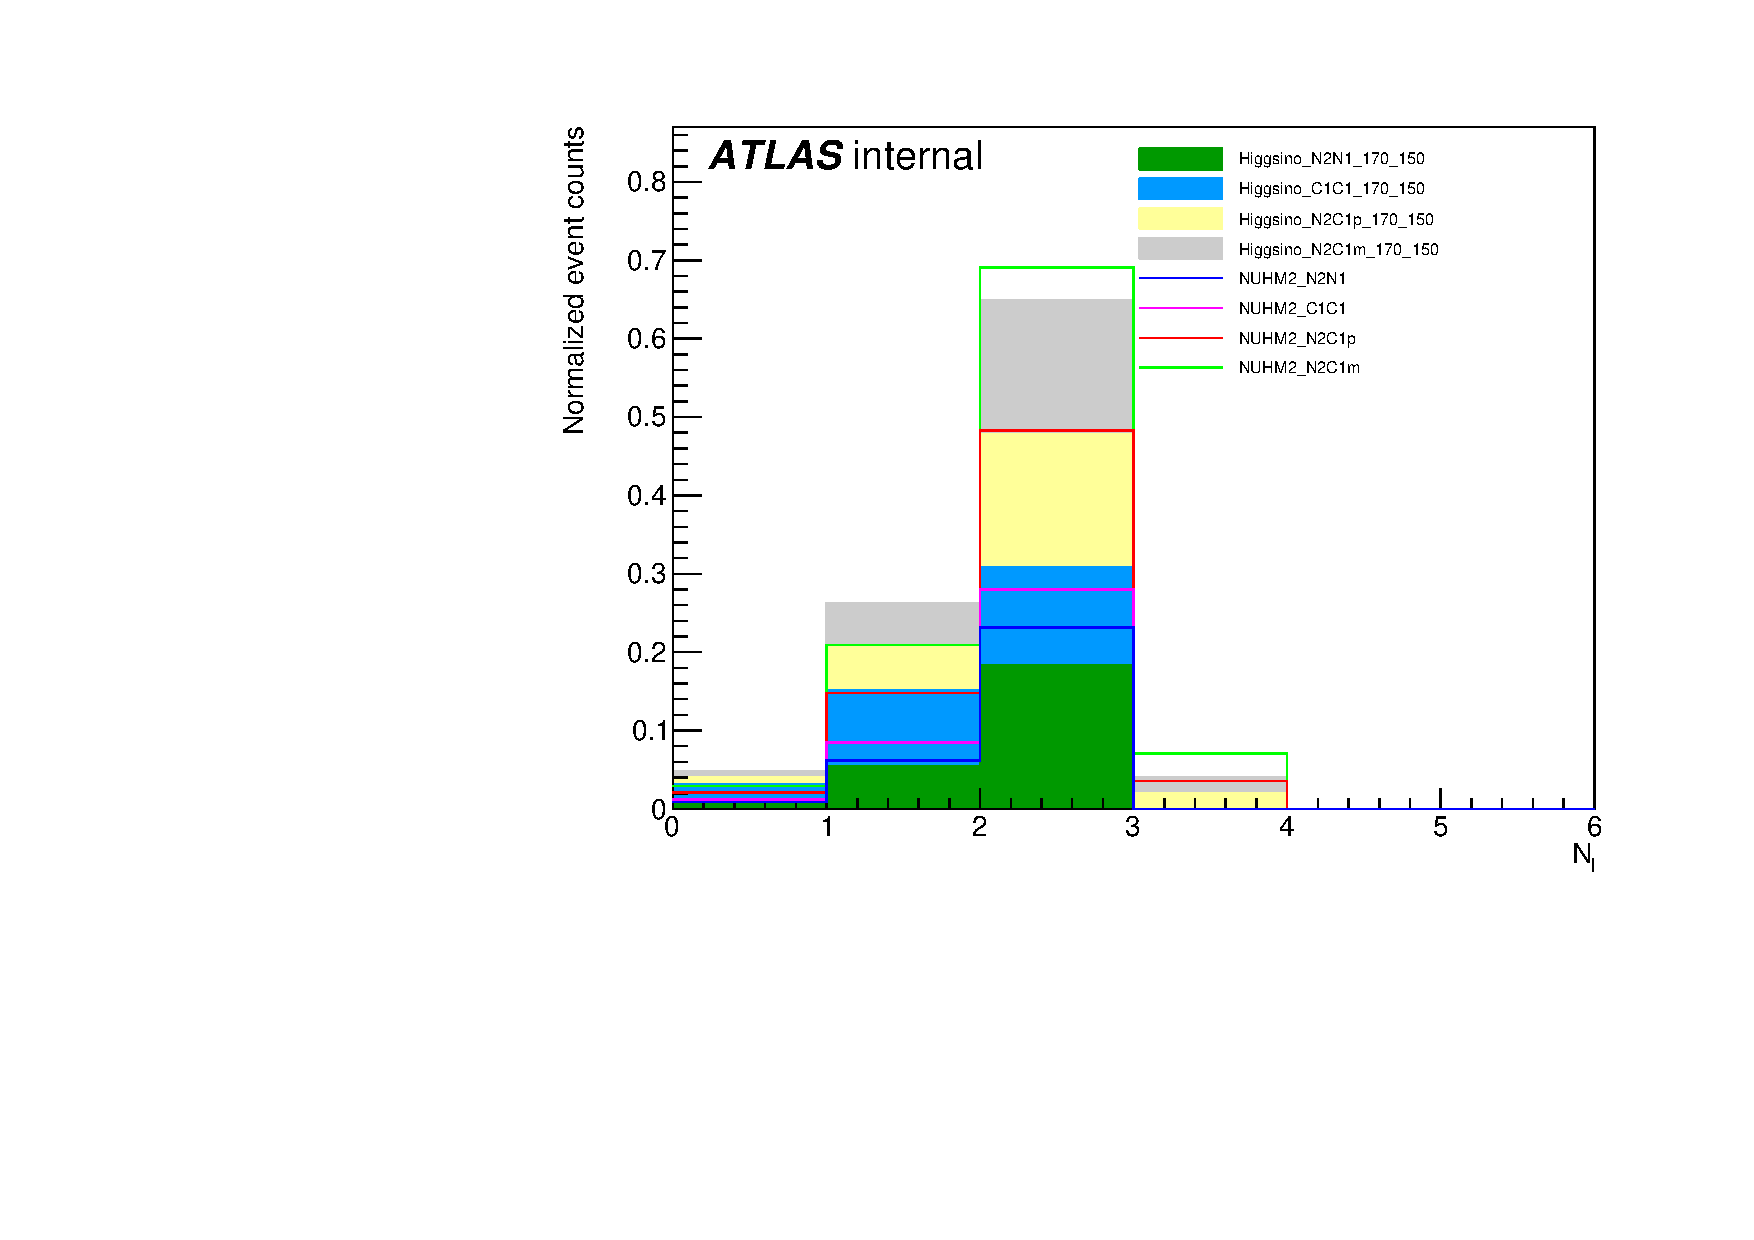
\includegraphics[scale=0.35]{nSignalLeptons.pdf}
            \caption{Signal leptons multiplicities}
        \end{subfigure}
        \begin{subfigure}[b]{0.48\textwidth}
            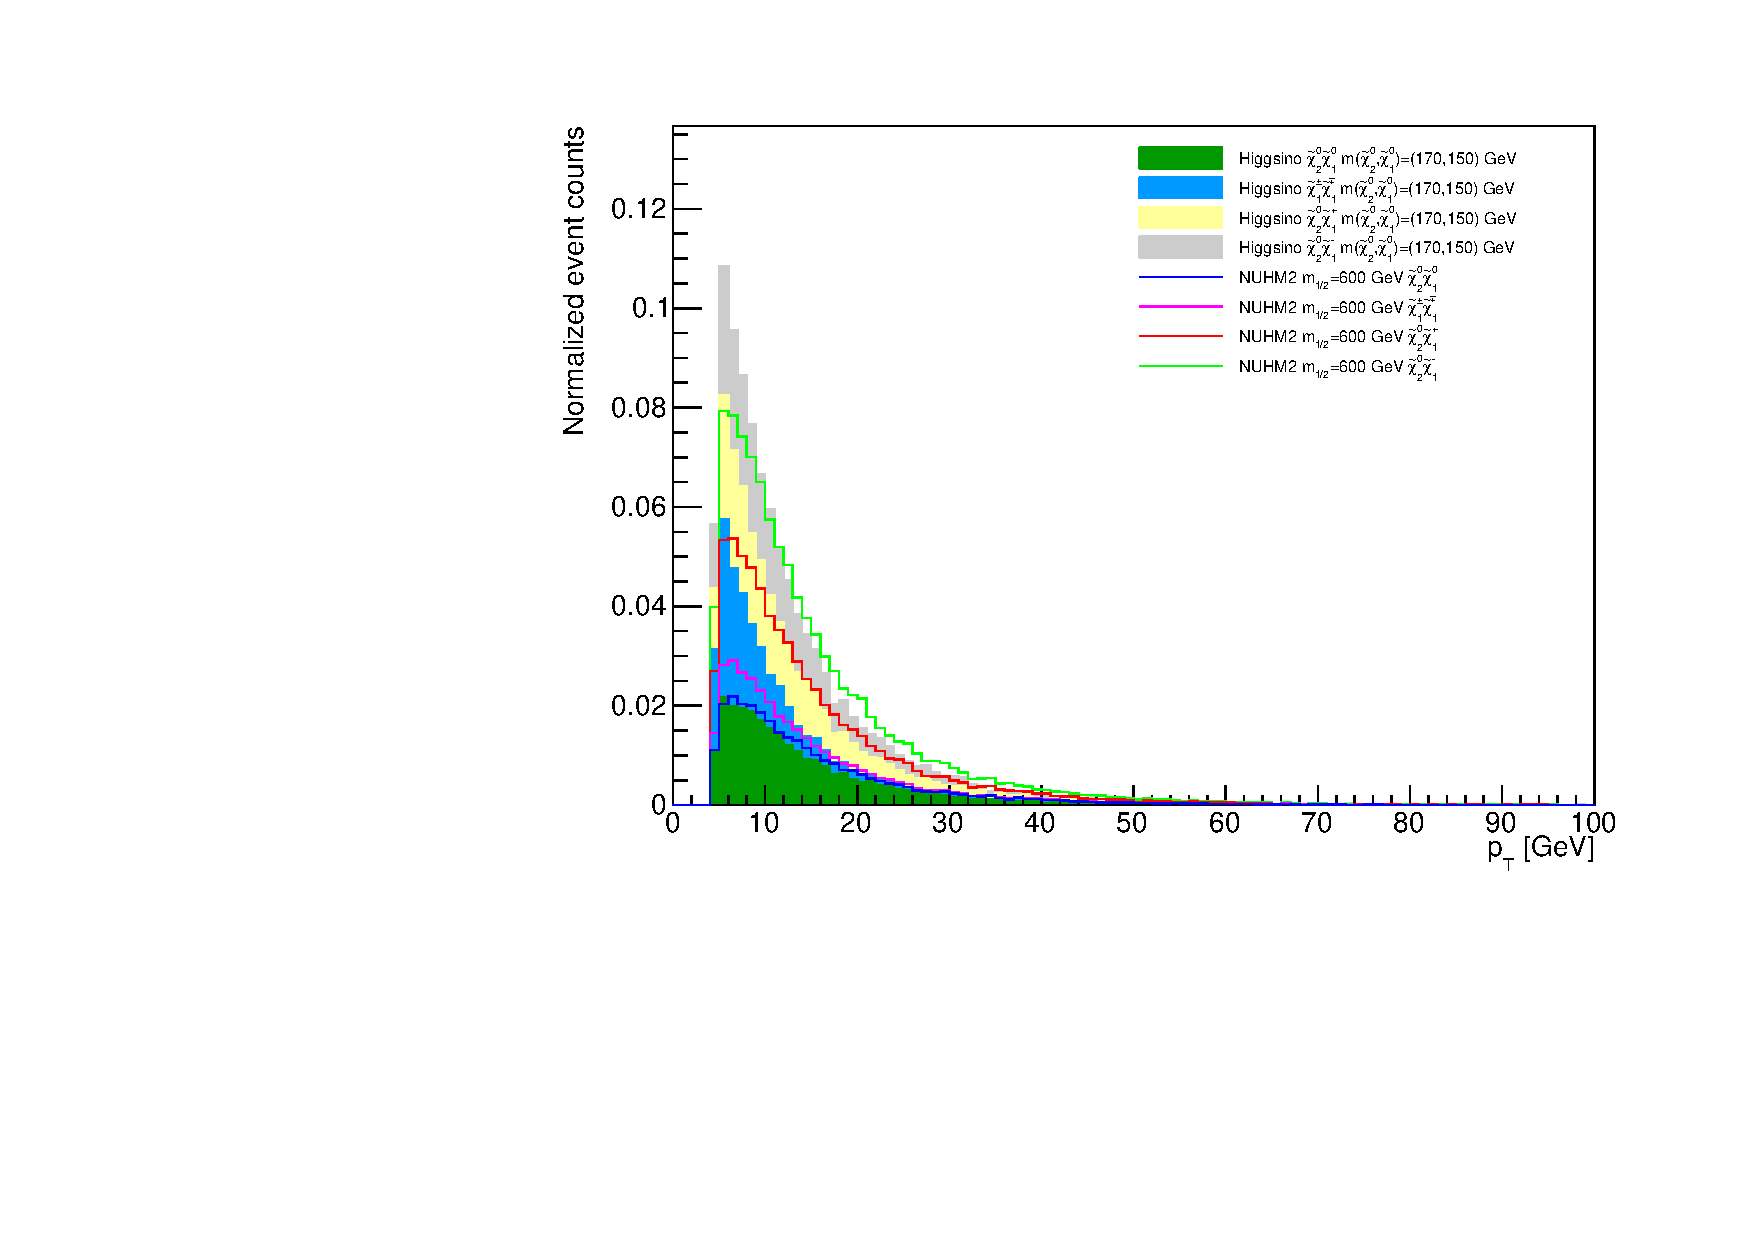
\includegraphics[scale=0.35]{signalElectrons_pt.pdf}
            \caption{Signal electrons \pt}
        \end{subfigure}
        \begin{subfigure}[b]{0.48\textwidth}
            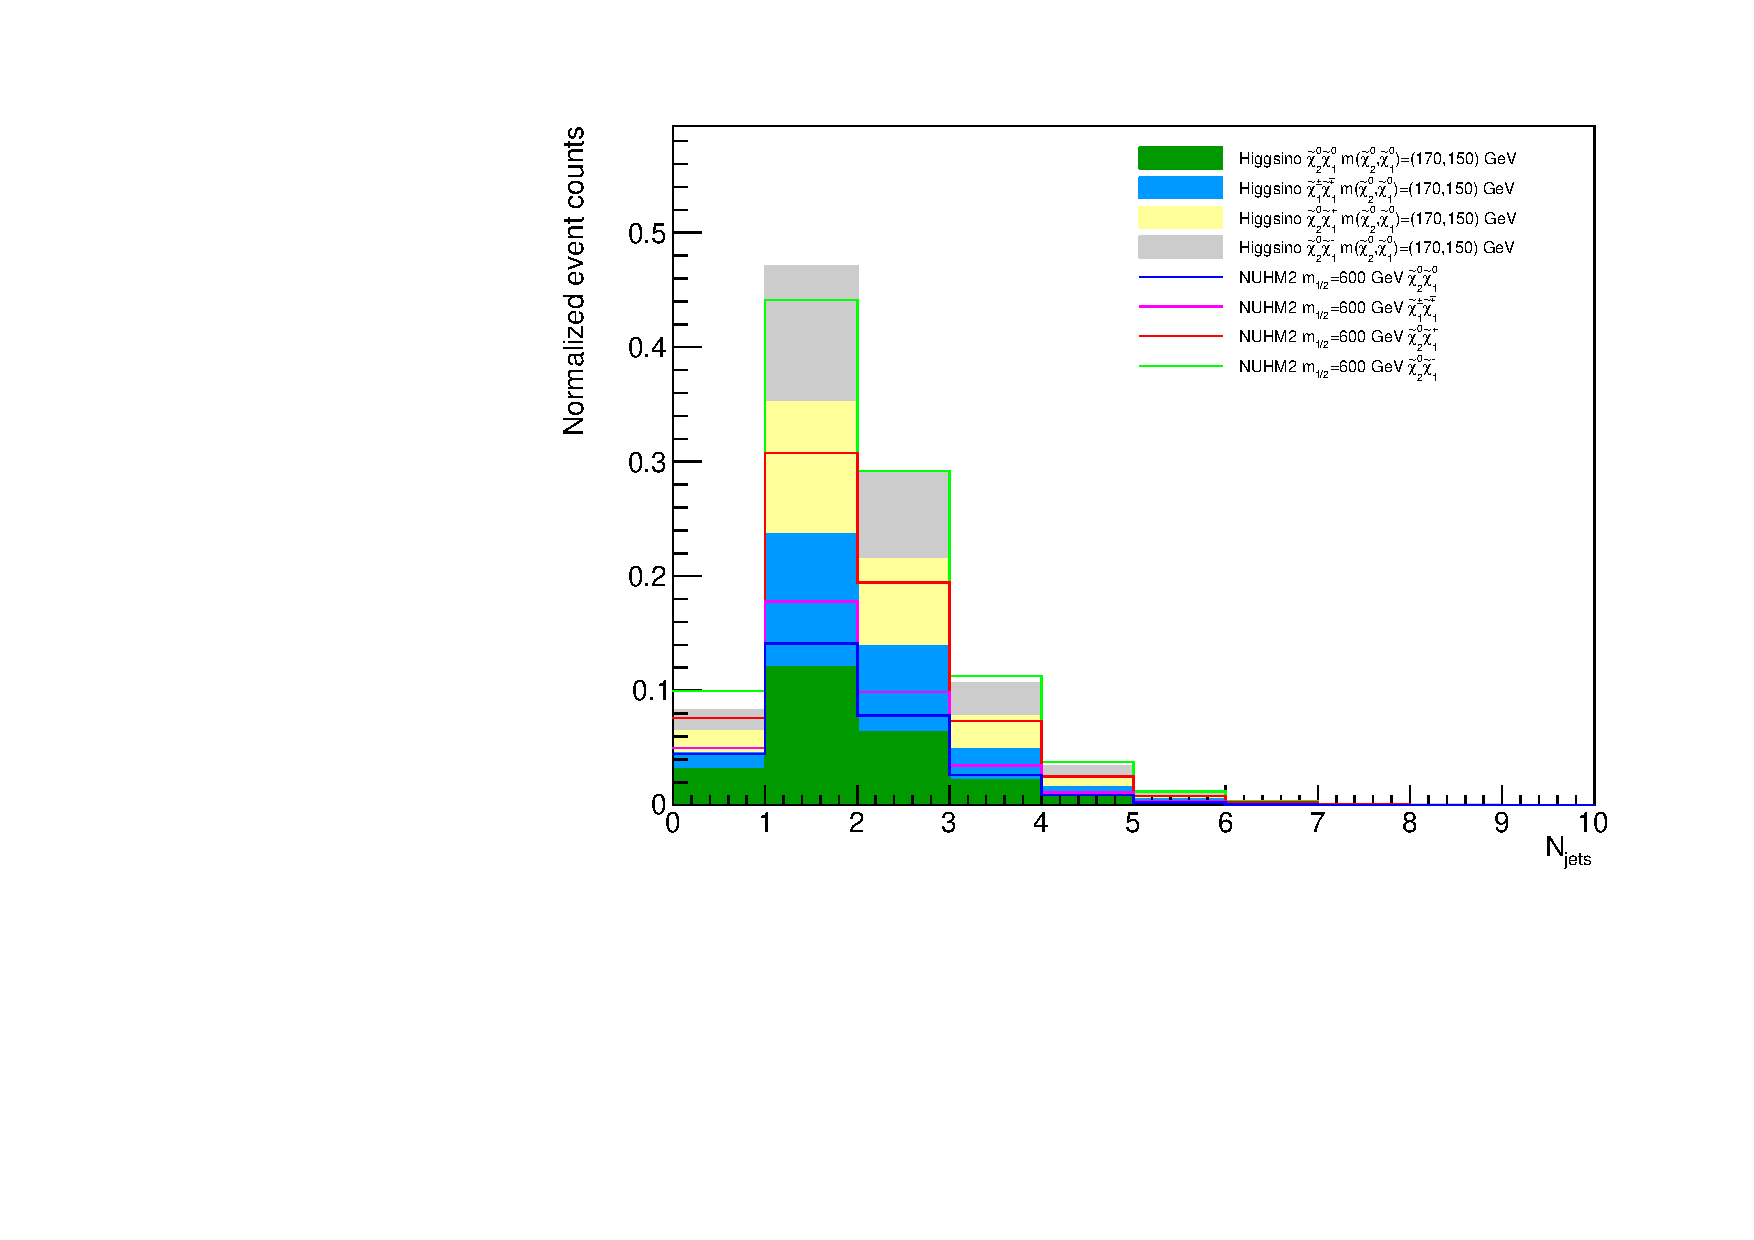
\includegraphics[scale=0.35]{nJets.pdf}
            \caption{Jets multiplicity}
        \end{subfigure}
        \begin{subfigure}[b]{0.48\textwidth}
            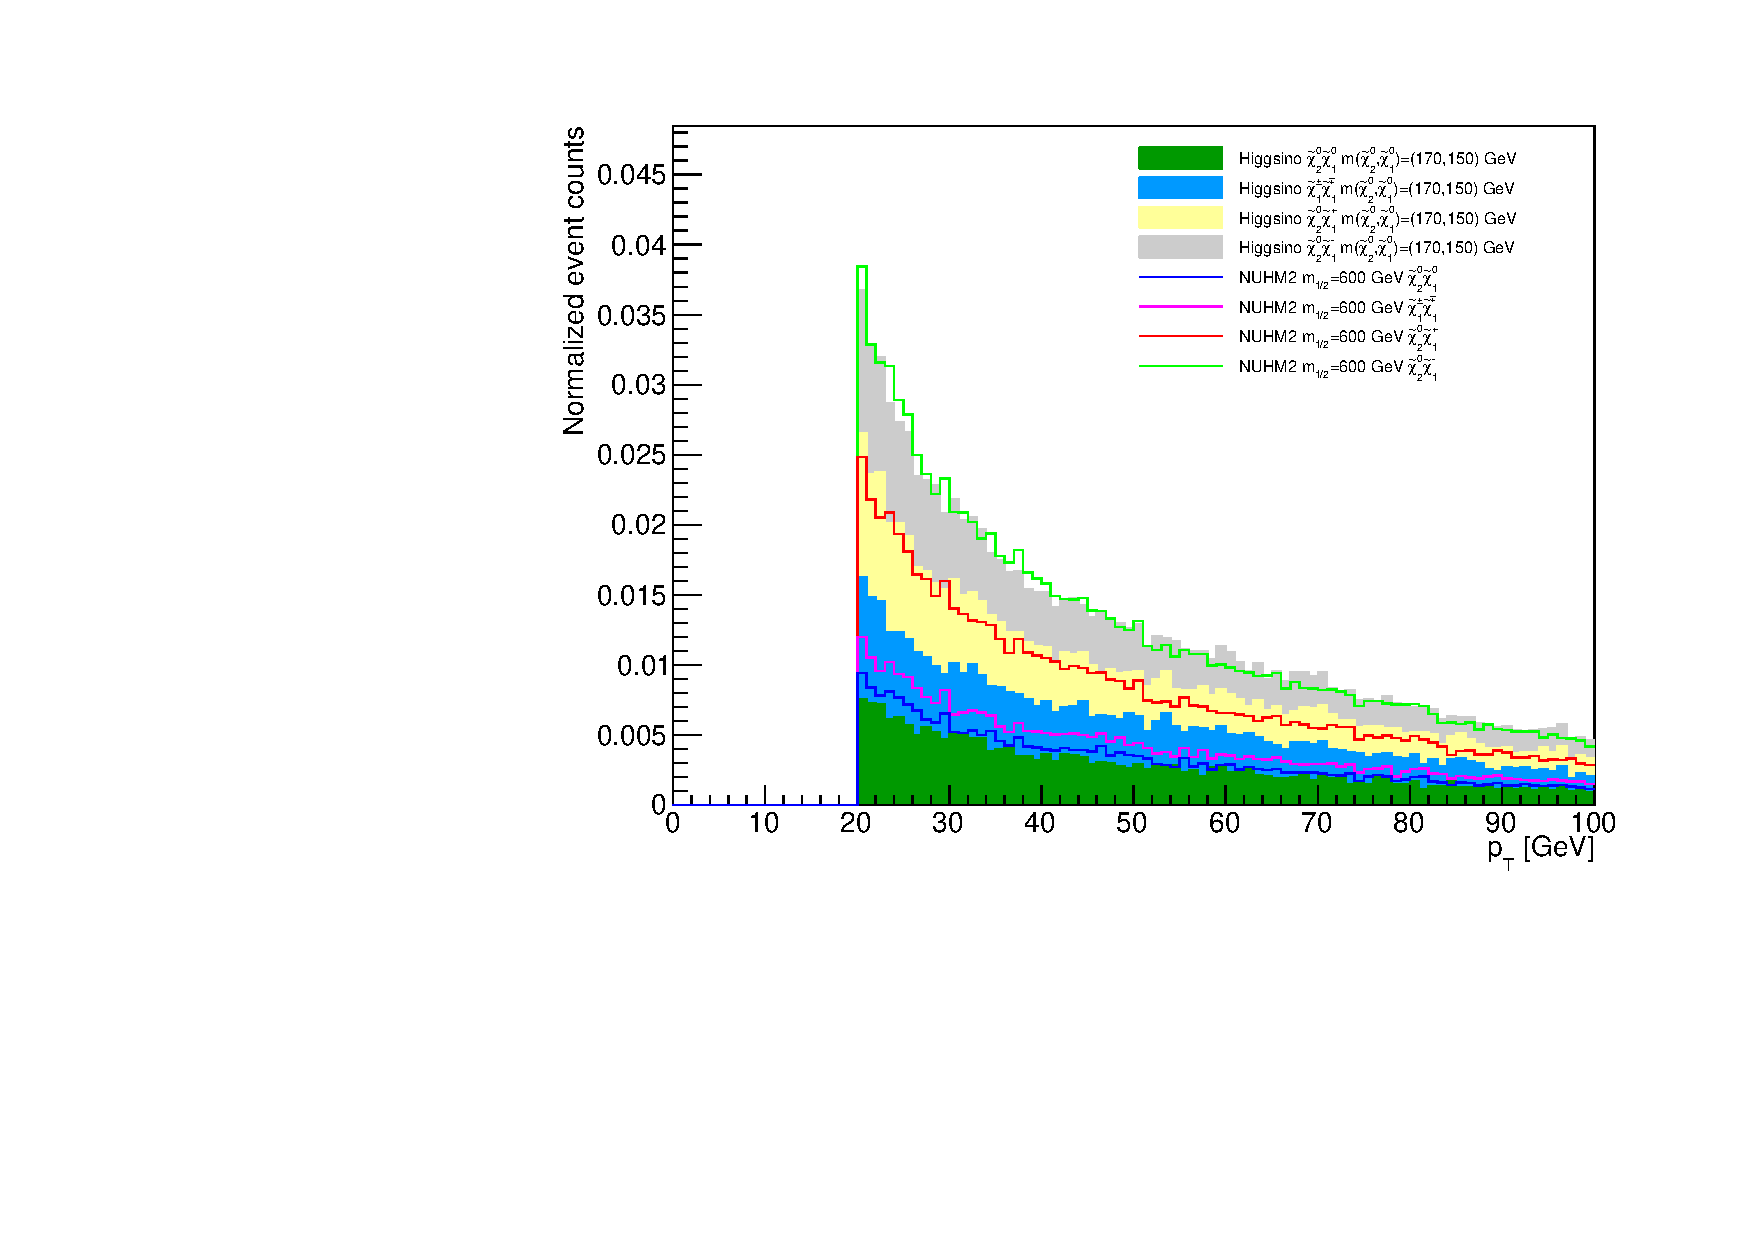
\includegraphics[scale=0.35]{signalJets_pt.pdf}
            \caption{Signal jets \pt.}
        \end{subfigure}
        \begin{subfigure}[b]{0.48\textwidth}
            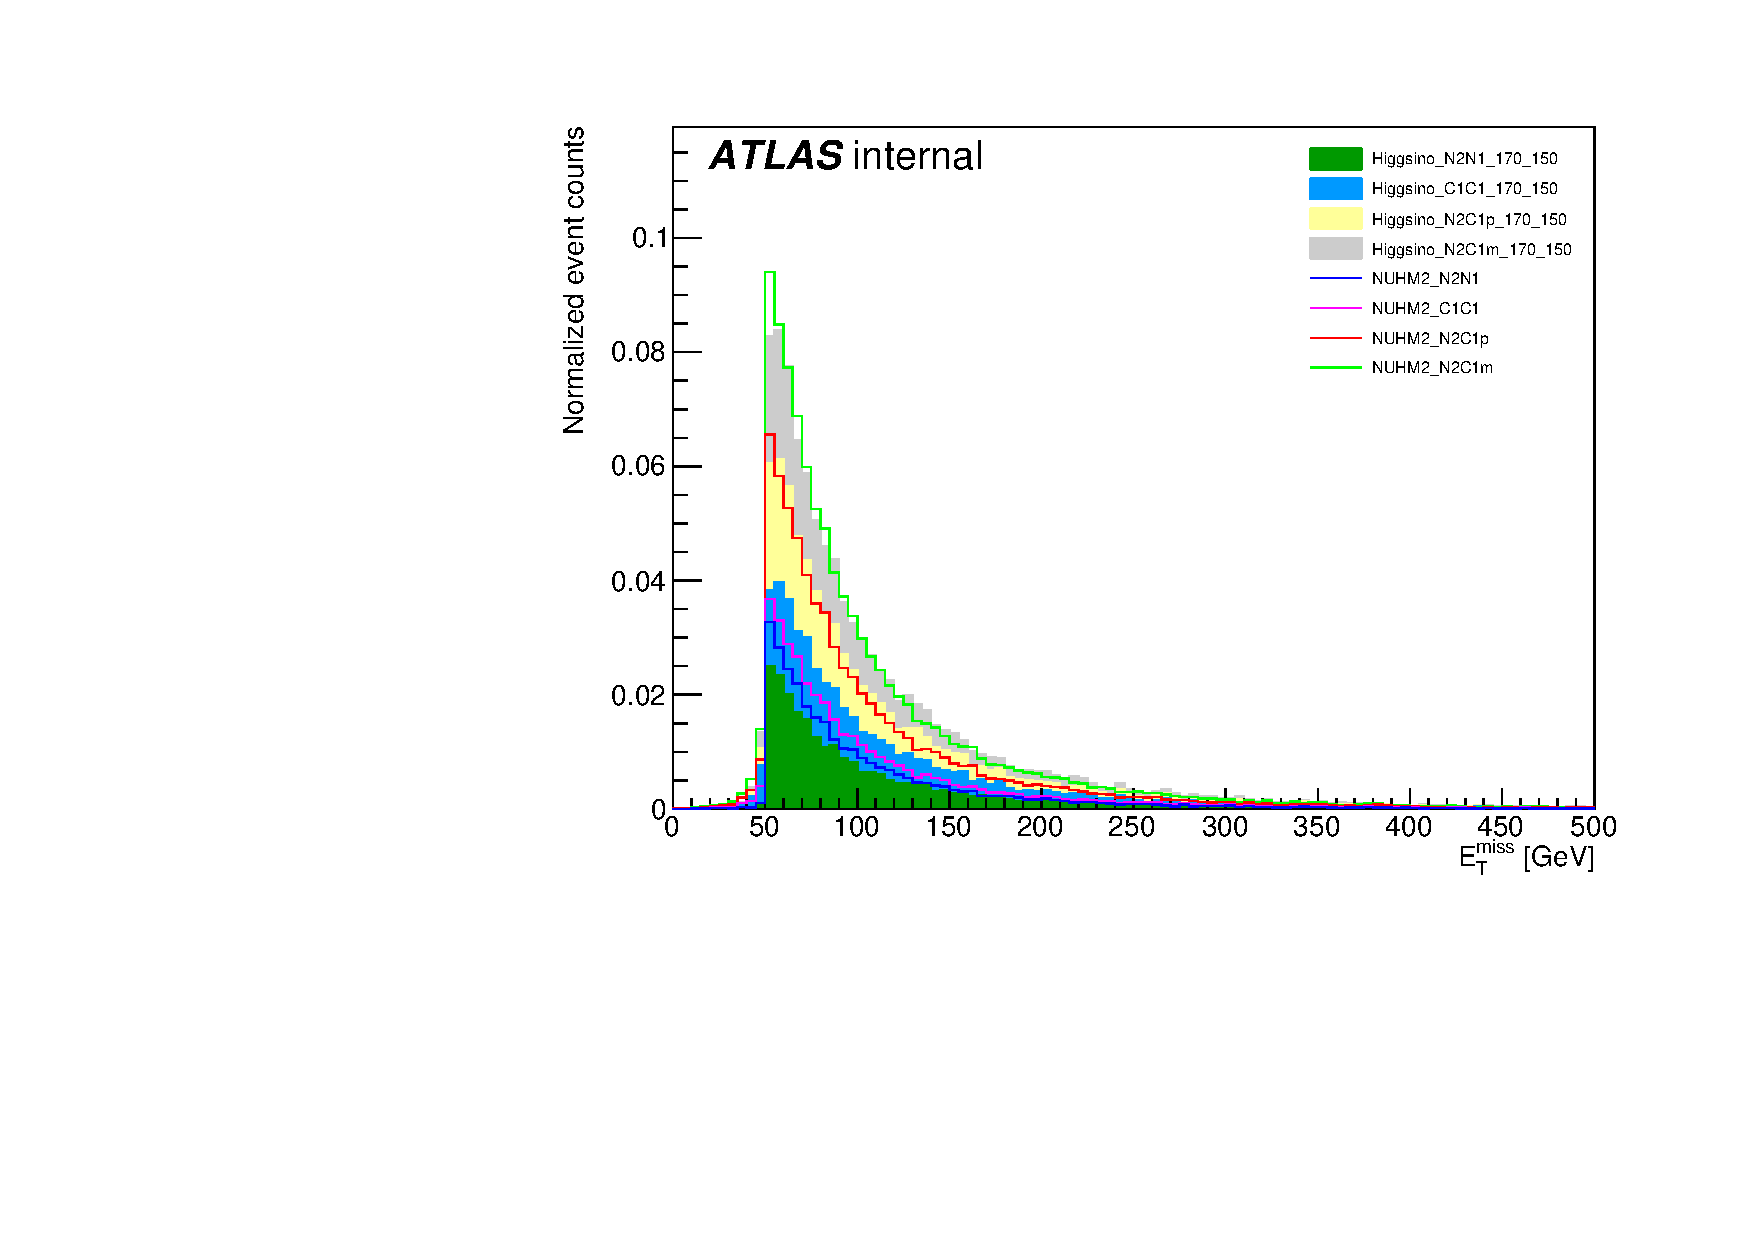
\includegraphics[scale=0.35]{met.pdf}
            \caption{\met}
        \end{subfigure}
        \begin{subfigure}[b]{0.48\textwidth}
            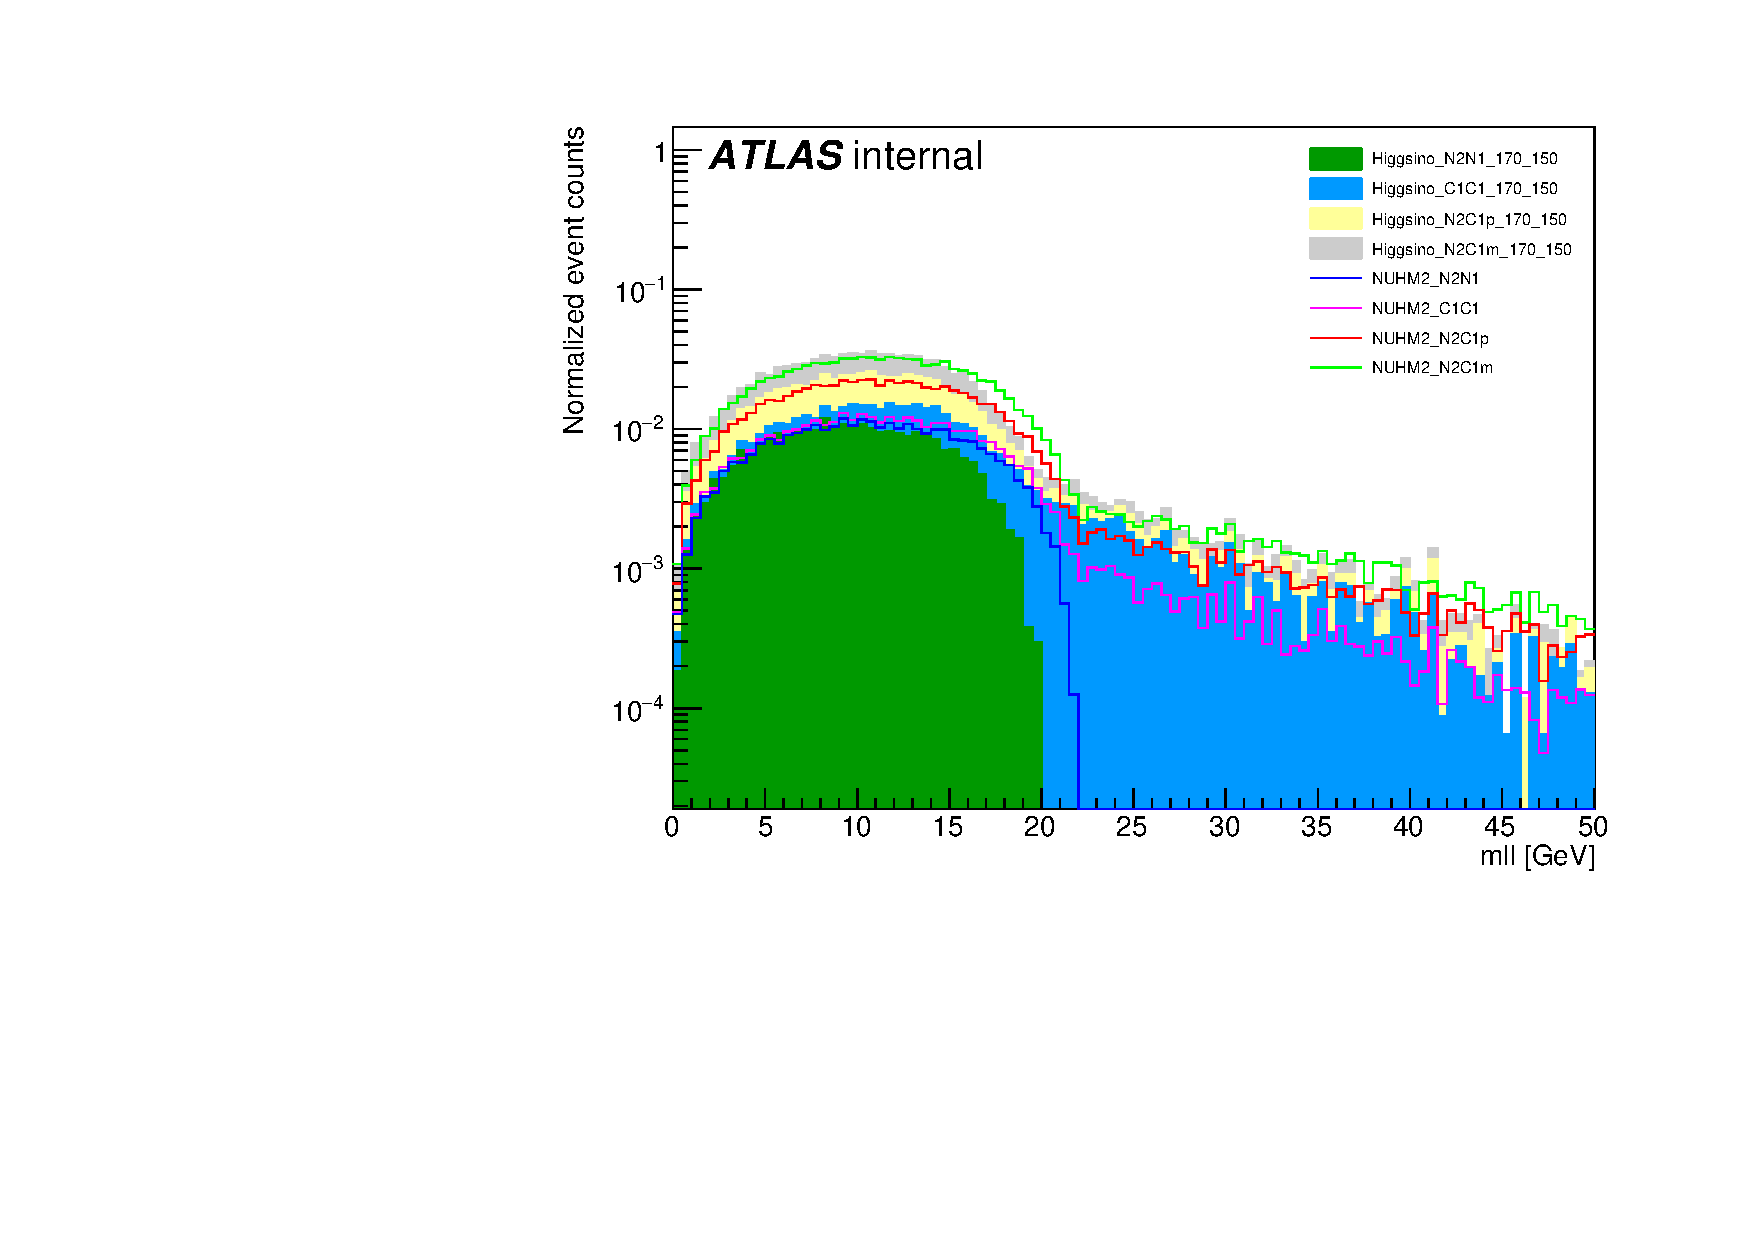
\includegraphics[scale=0.35]{mll.pdf}
            \caption{$m_{\ell\ell}$}
        \end{subfigure}
    \end{center}
    \caption{The kinematic distribution comparisons in truth level using the NUHM2 samples with $m_{1/2} = 600$~{\GeV} and the simplified Higgsino samples with $m_{\widetilde{\chi}^{0}_{2}} = 170$~{\GeV}, $m_{\widetilde{\chi}^{0}_{1}} = 150$~{\GeV}.
    Four different production channels, $\widetilde{\chi}^{0}_{2}\widetilde{\chi}^{0}_{1}$, $\widetilde{\chi}^{0}_{2}\widetilde{\chi}^{+}_{1}$, $\widetilde{\chi}^{0}_{2}\widetilde{\chi}^{-}_{1}$, and $\widetilde{\chi}^{\pm}_{1}\widetilde{\chi}^{\mp}_{1}$, for the NUHM2 and the simplified Higgsino model are considered.
    The distributions of four productions are combined and normalized to equal area.}
    \label{fig:results_kinematic_distribution_comparisons}
\end{figure}

% \begin{figure}[htbp]
%     \begin{center}
%         \begin{subfigure}[b]{0.48\textwidth}
%             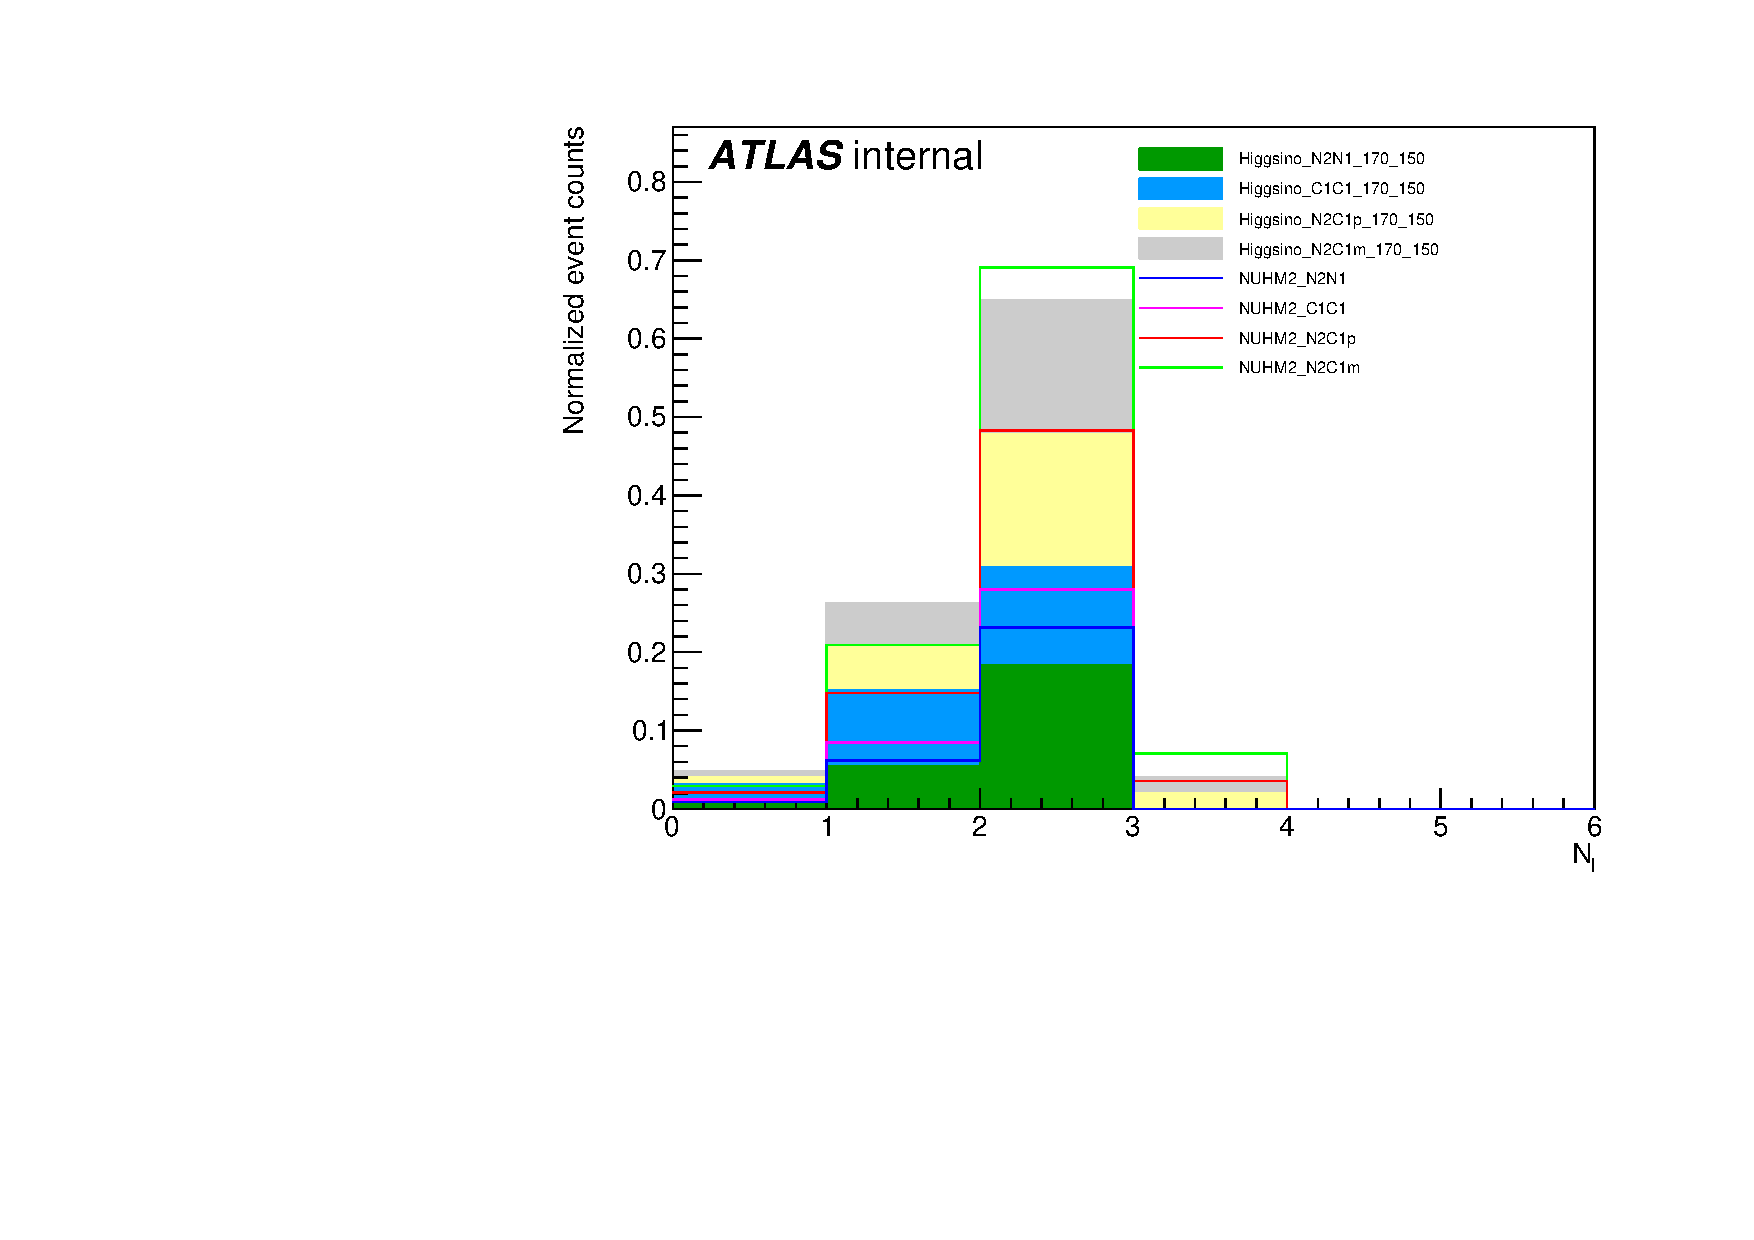
\includegraphics[scale=0.4]{nBaselineLeptons.pdf}
%             \caption{Baseline leptons multiplicities}
%         \end{subfigure}
%         \begin{subfigure}[b]{0.48\textwidth}
%             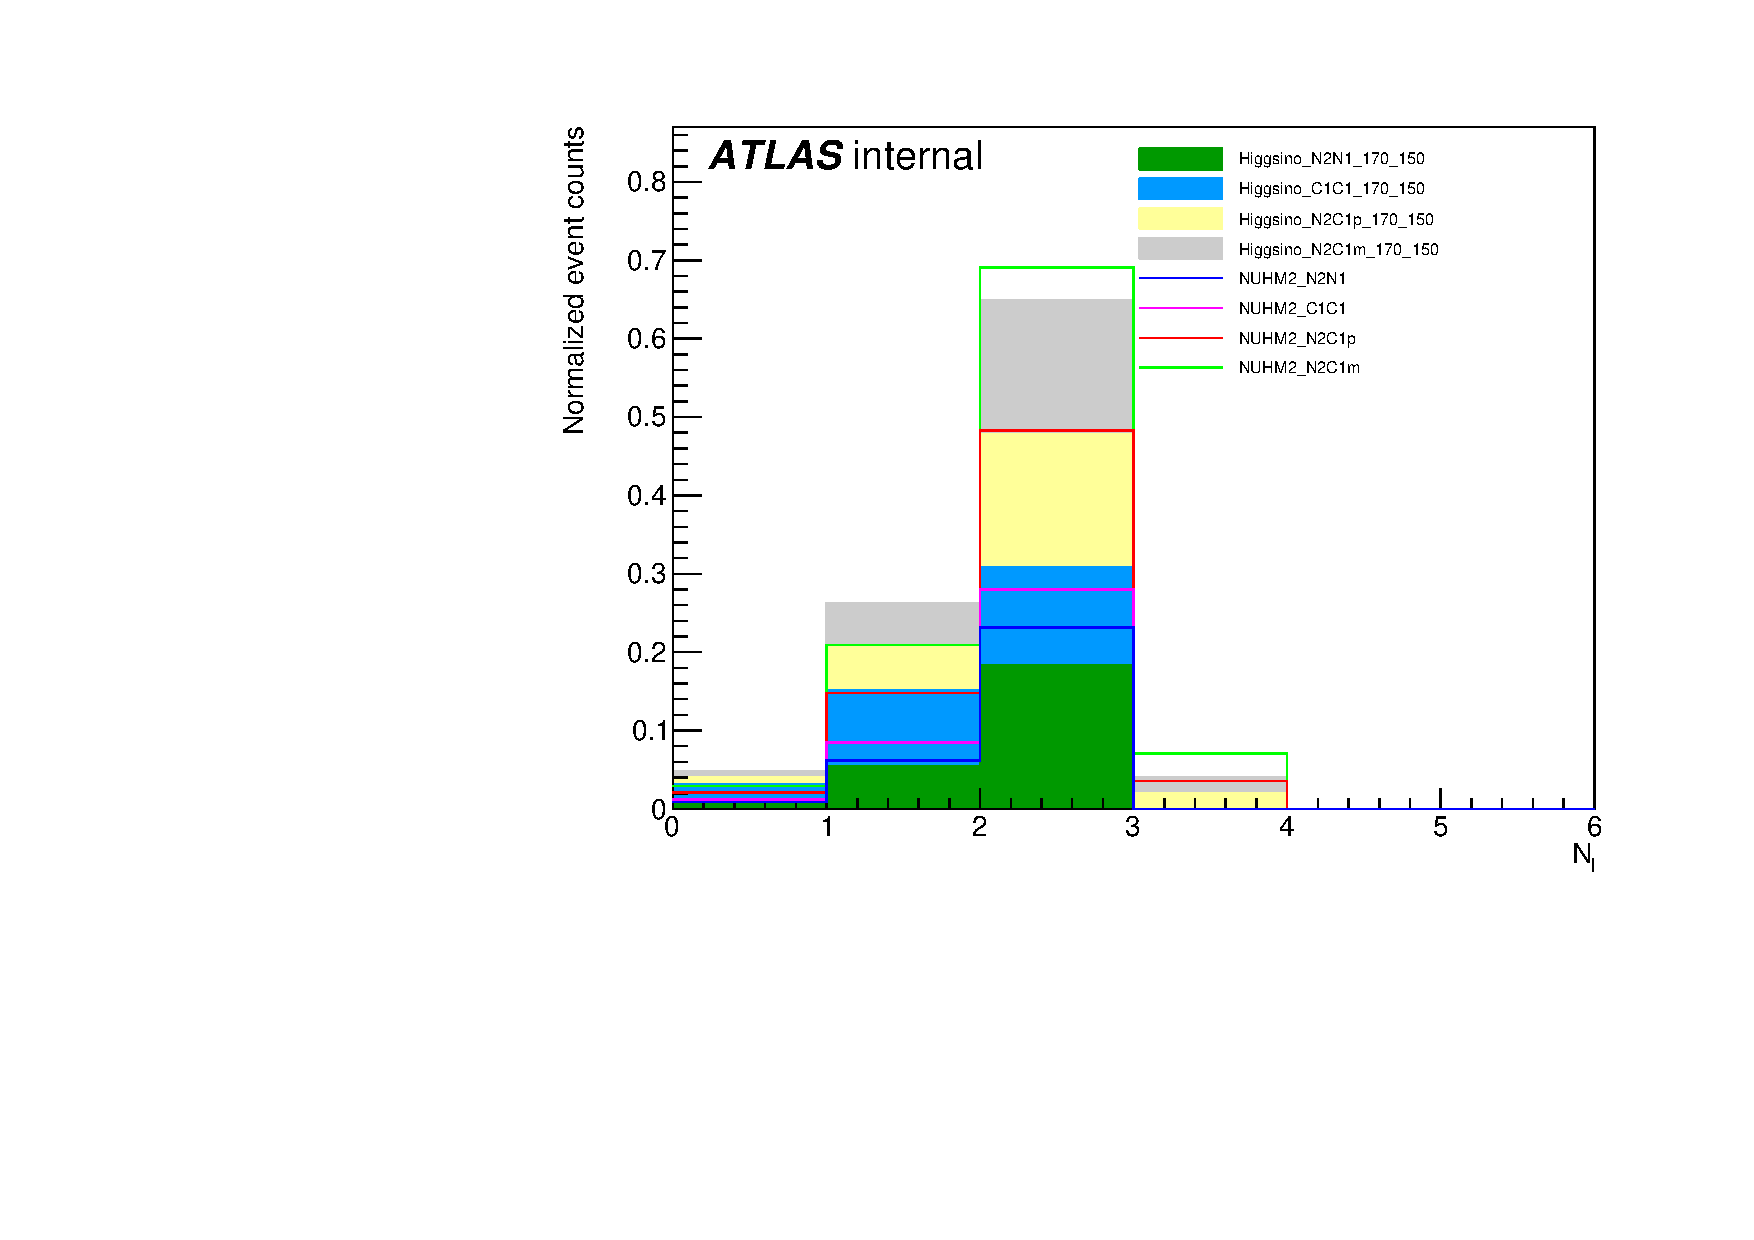
\includegraphics[scale=0.4]{nSignalLeptons.pdf}
%             \caption{Signal leptons multiplicities}
%         \end{subfigure}
%         \begin{subfigure}[b]{0.48\textwidth}
%             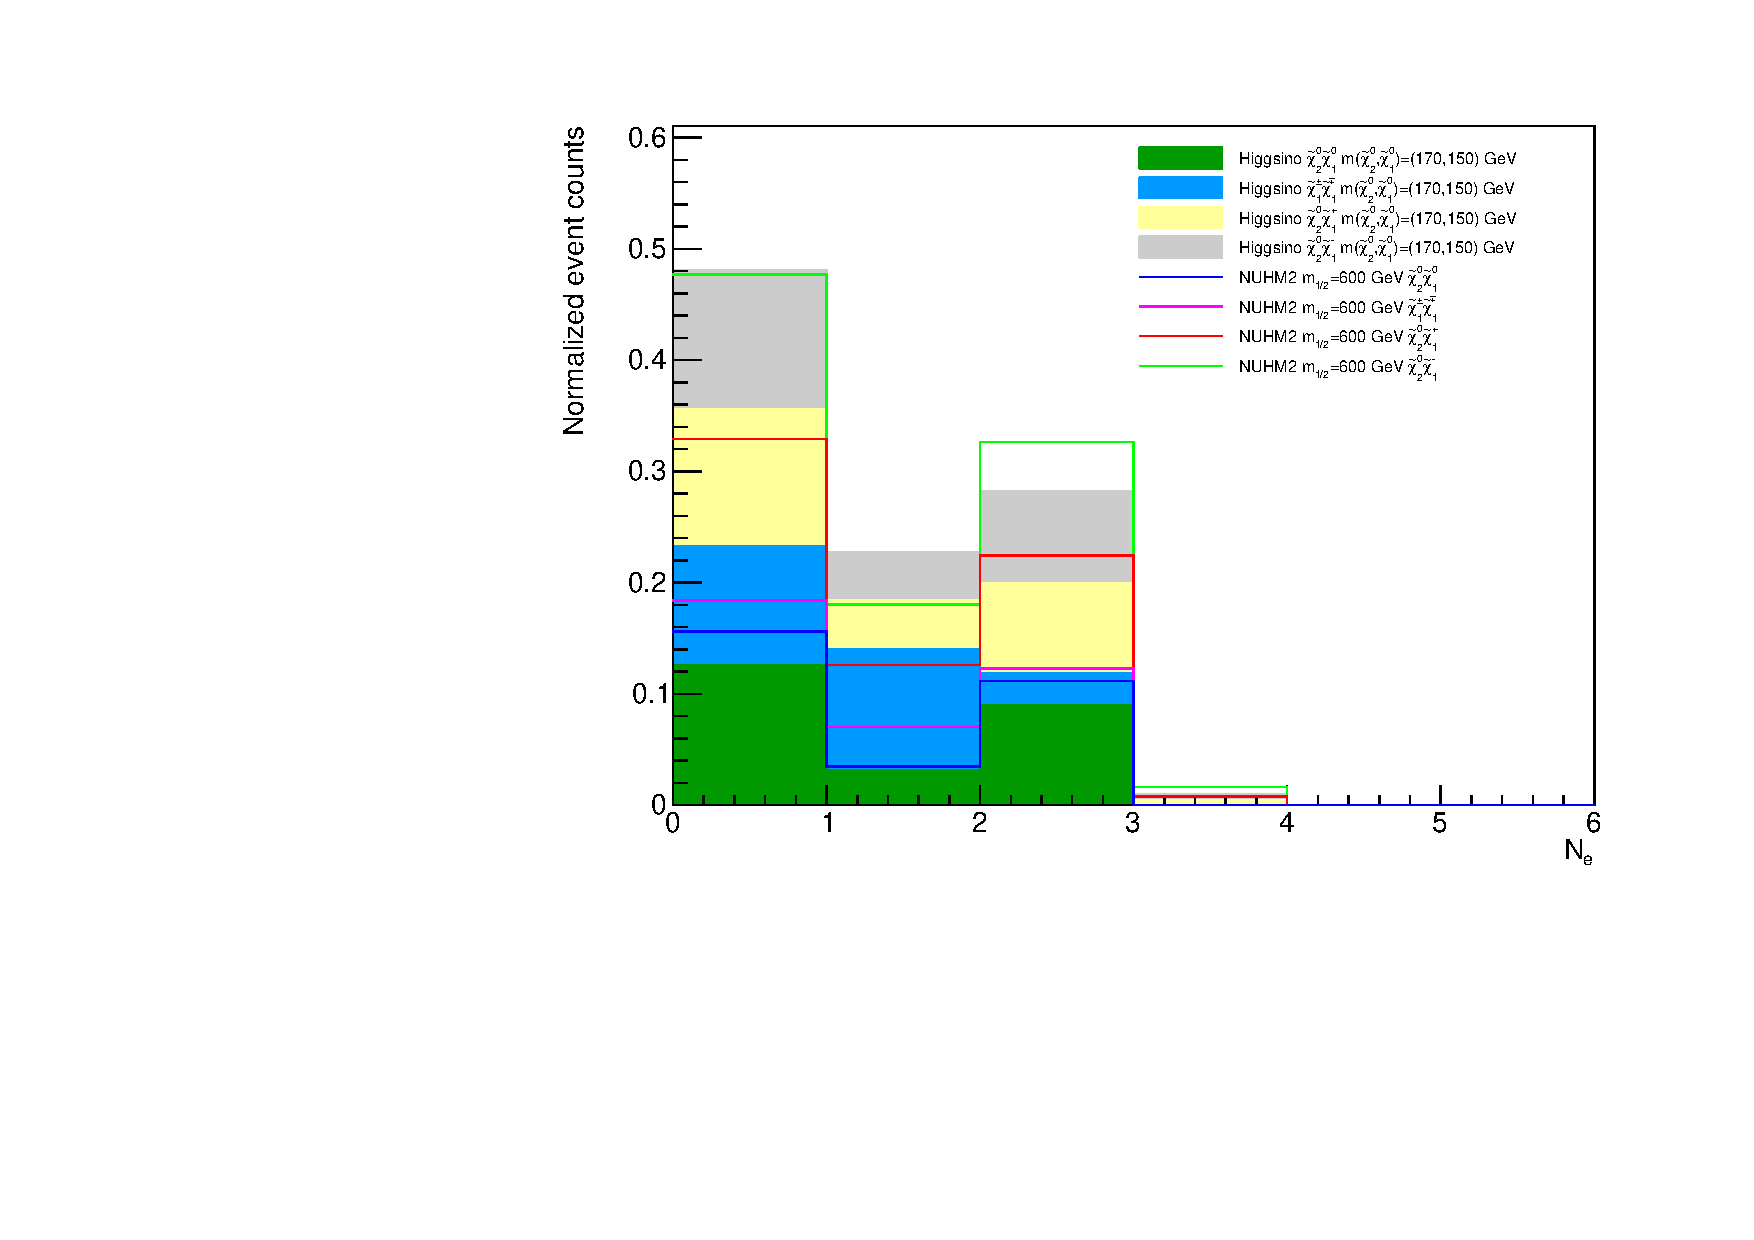
\includegraphics[scale=0.4]{nElectrons.pdf}
%             \caption{Signal electrons multiplicities}
%         \end{subfigure}
%         \begin{subfigure}[b]{0.48\textwidth}
%             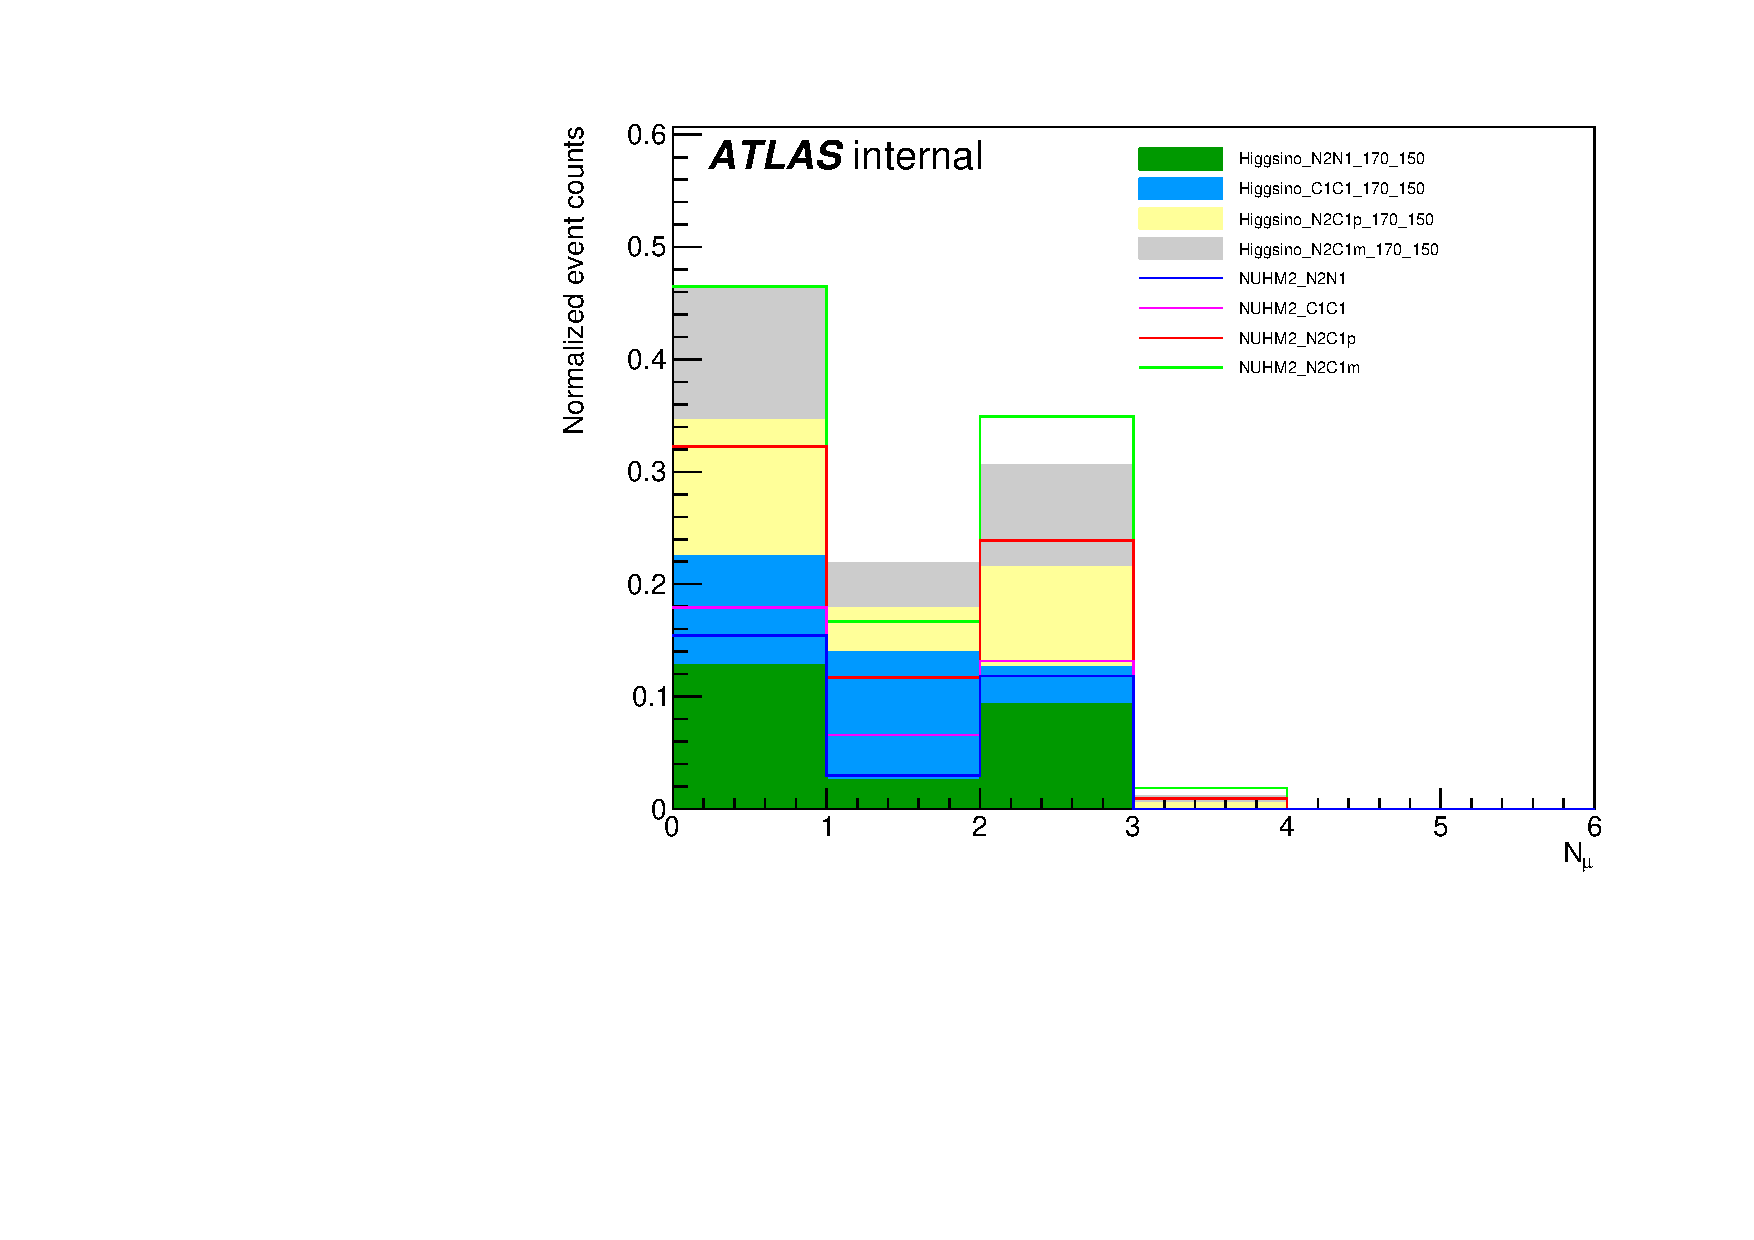
\includegraphics[scale=0.4]{nMuons.pdf}
%             \caption{Signal muons multiplicities}
%         \end{subfigure}
%     \end{center}
%     \caption{The lepton multiplicity distributions.
%     The lepton multiplicity of NUHM2 with $m_{1/2} = 600$~{\GeV} are compared to the simplified Higgsino model with $m_{\widetilde{\chi}^{0}_{2}}=170$~{\GeV} and $m_{\widetilde{\chi}^{0}_{1}}=150$~{\GeV}.
%     Four different production channels, $\widetilde{\chi}^{0}_{2}\widetilde{\chi}^{0}_{1}$, $\widetilde{\chi}^{0}_{2}\widetilde{\chi}^{+}_{1}$, $\widetilde{\chi}^{0}_{2}\widetilde{\chi}^{-}_{1}$, and $\widetilde{\chi}^{\pm}_{1}\widetilde{\chi}^{\mp}_{1}$, for the NUHM2 and the simplified Higgsino model are considered.
%     The distributions of four productions are combined and normalized to equal area.}
%     \label{fig:results_nuhm2_lepton_multiplicity}
% \end{figure}

% \begin{figure}[htbp]
%     \begin{center}
%         \begin{subfigure}[b]{0.48\textwidth}
%             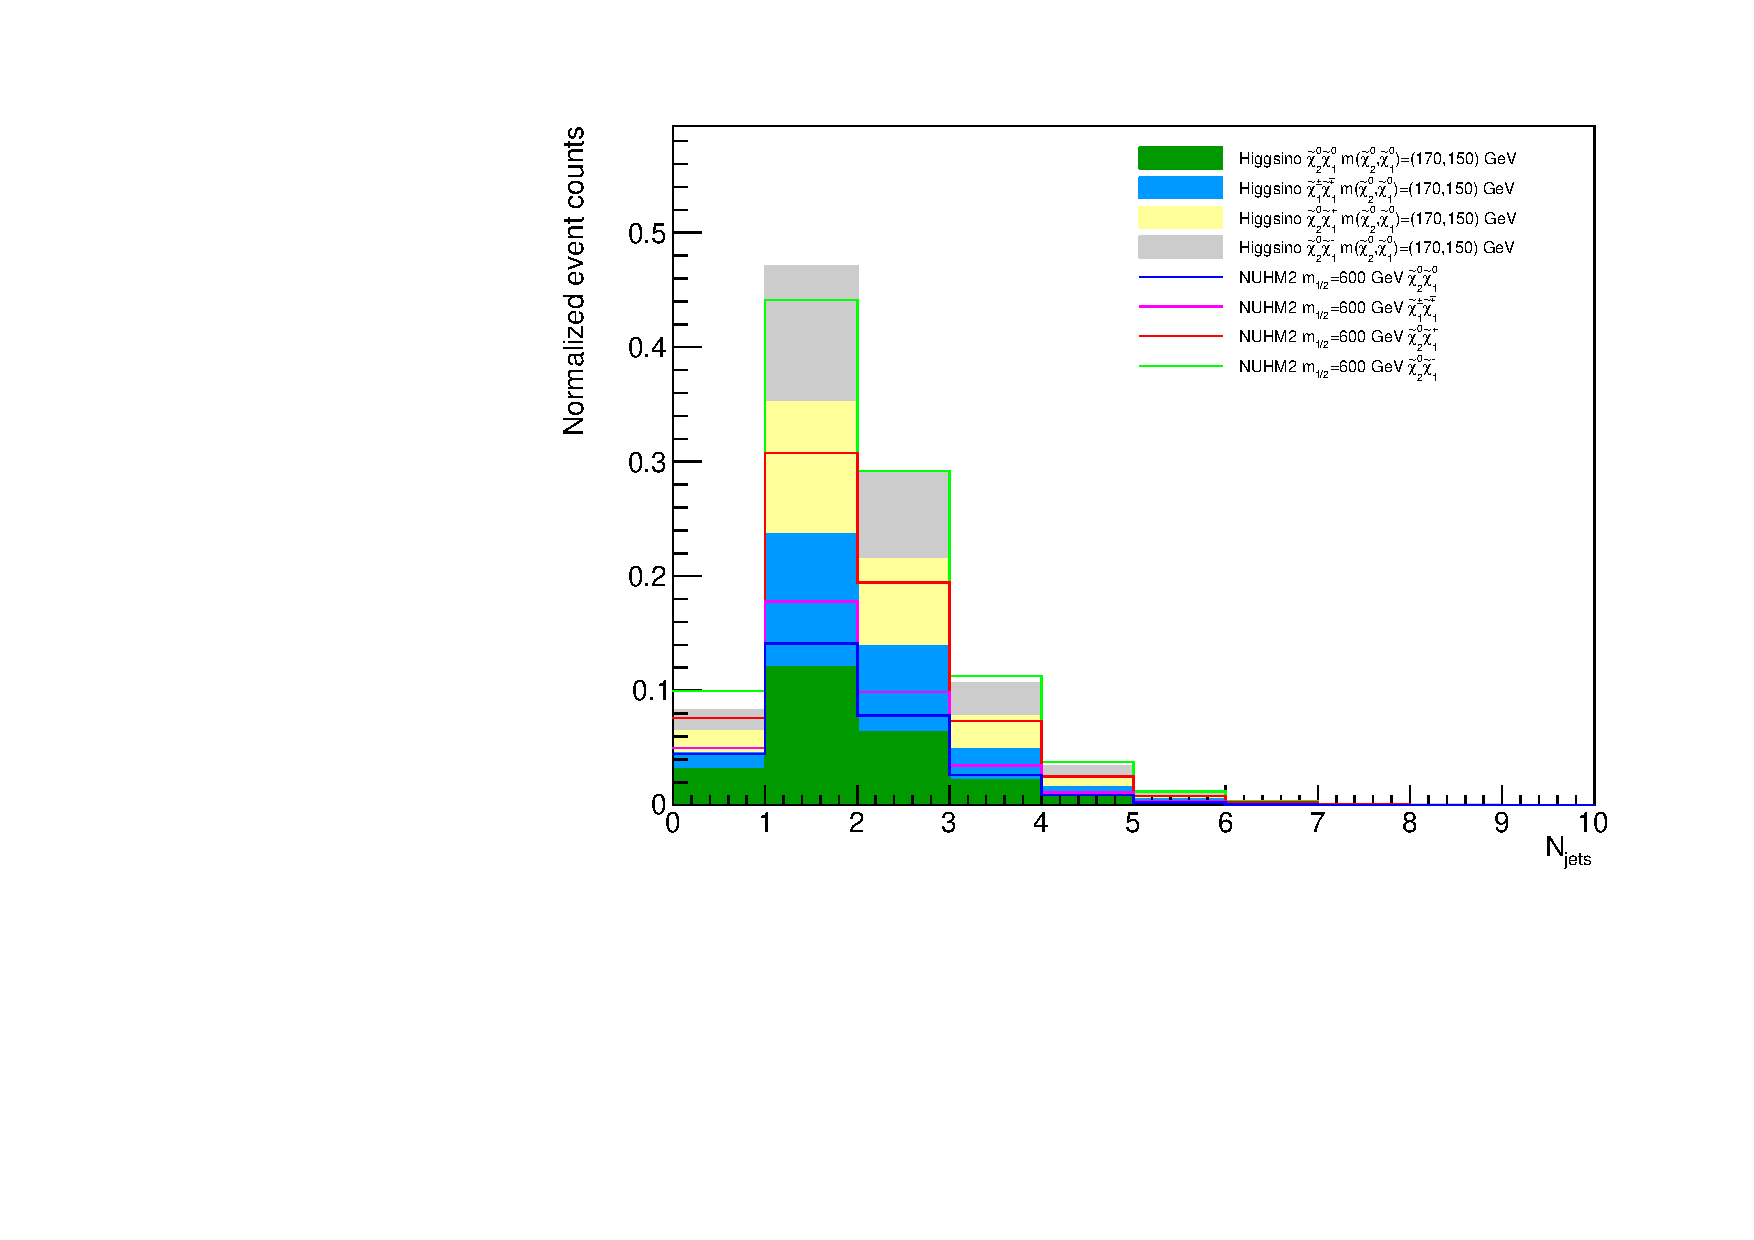
\includegraphics[scale=0.4]{nJets.pdf}
%             \caption{Jets multiplicity}
%         \end{subfigure}
%         \begin{subfigure}[b]{0.48\textwidth}
%             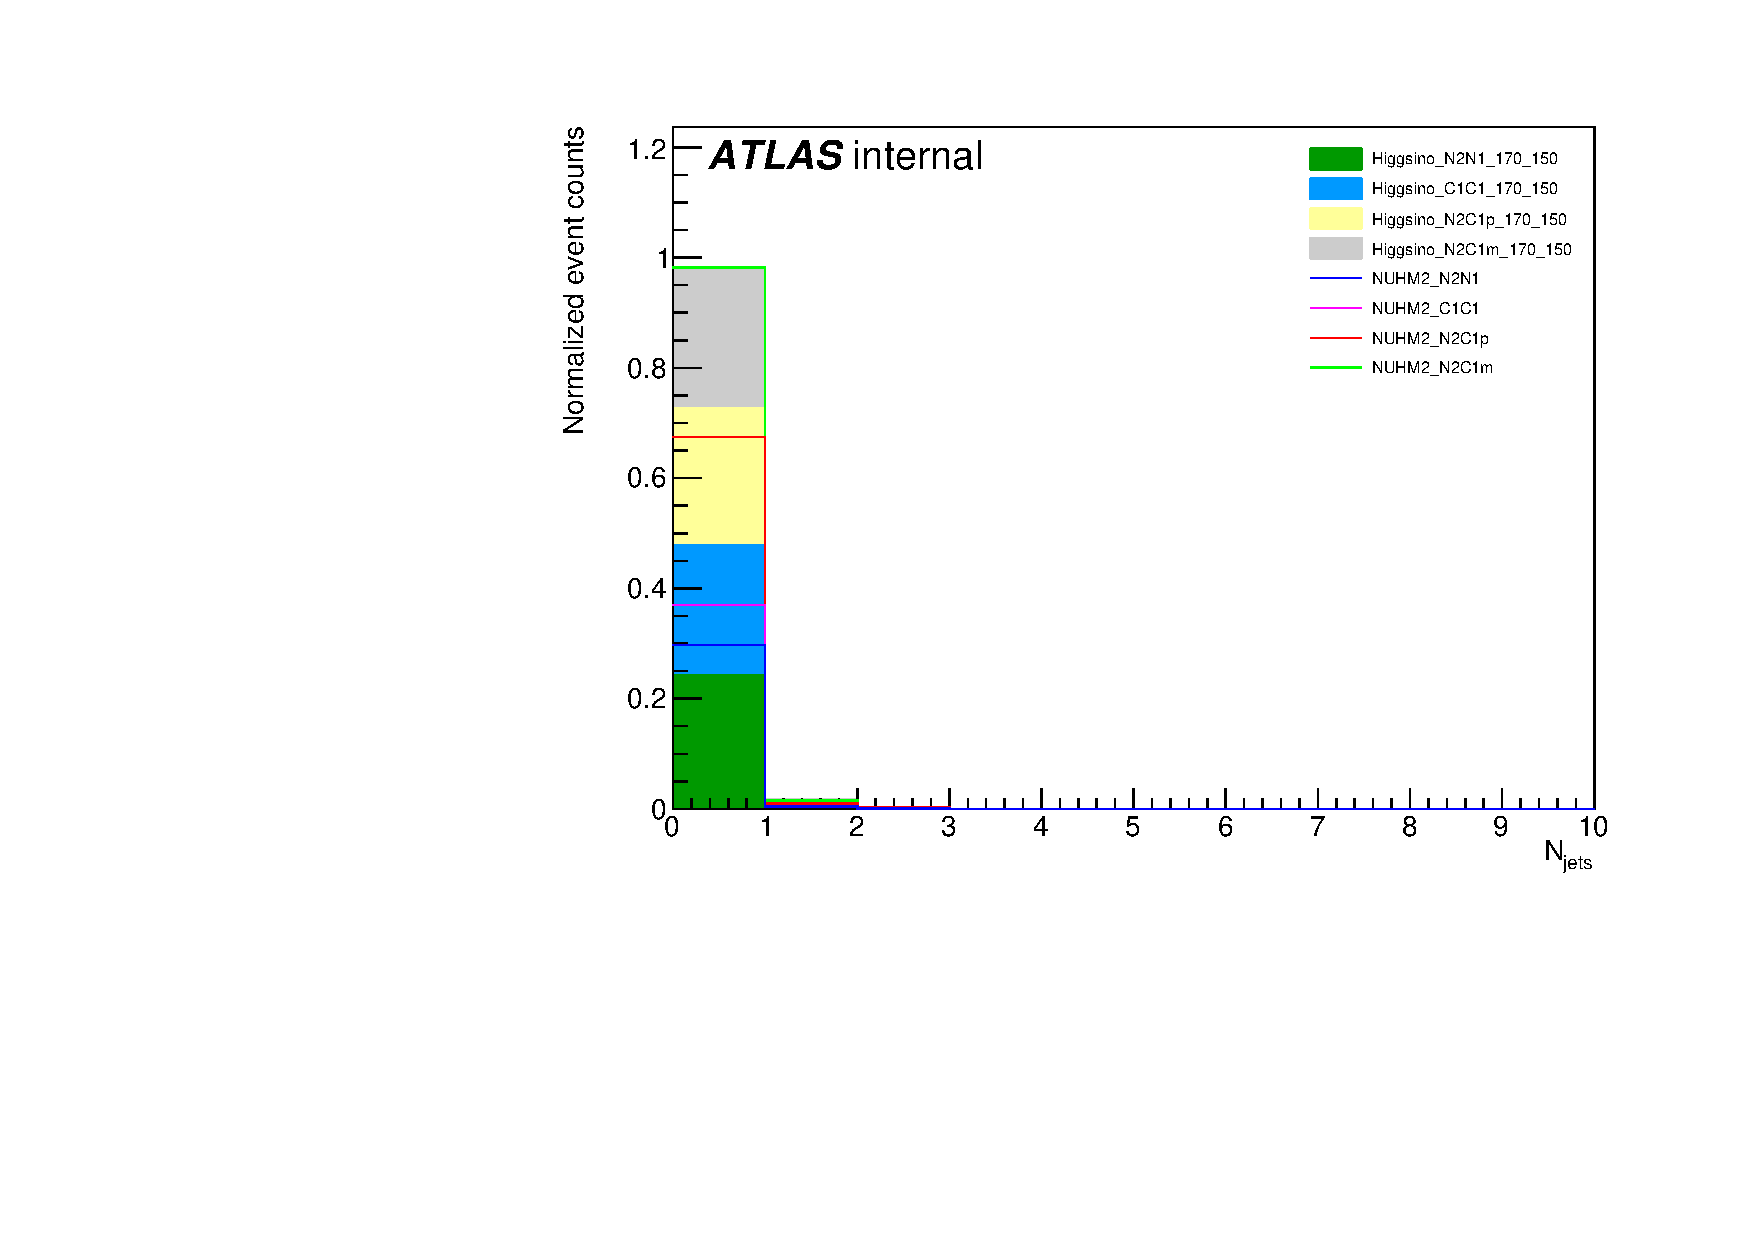
\includegraphics[scale=0.4]{nBjets.pdf}
%             \caption{$b$-jets multiplicity}
%         \end{subfigure}
%         \begin{subfigure}[b]{0.48\textwidth}
%             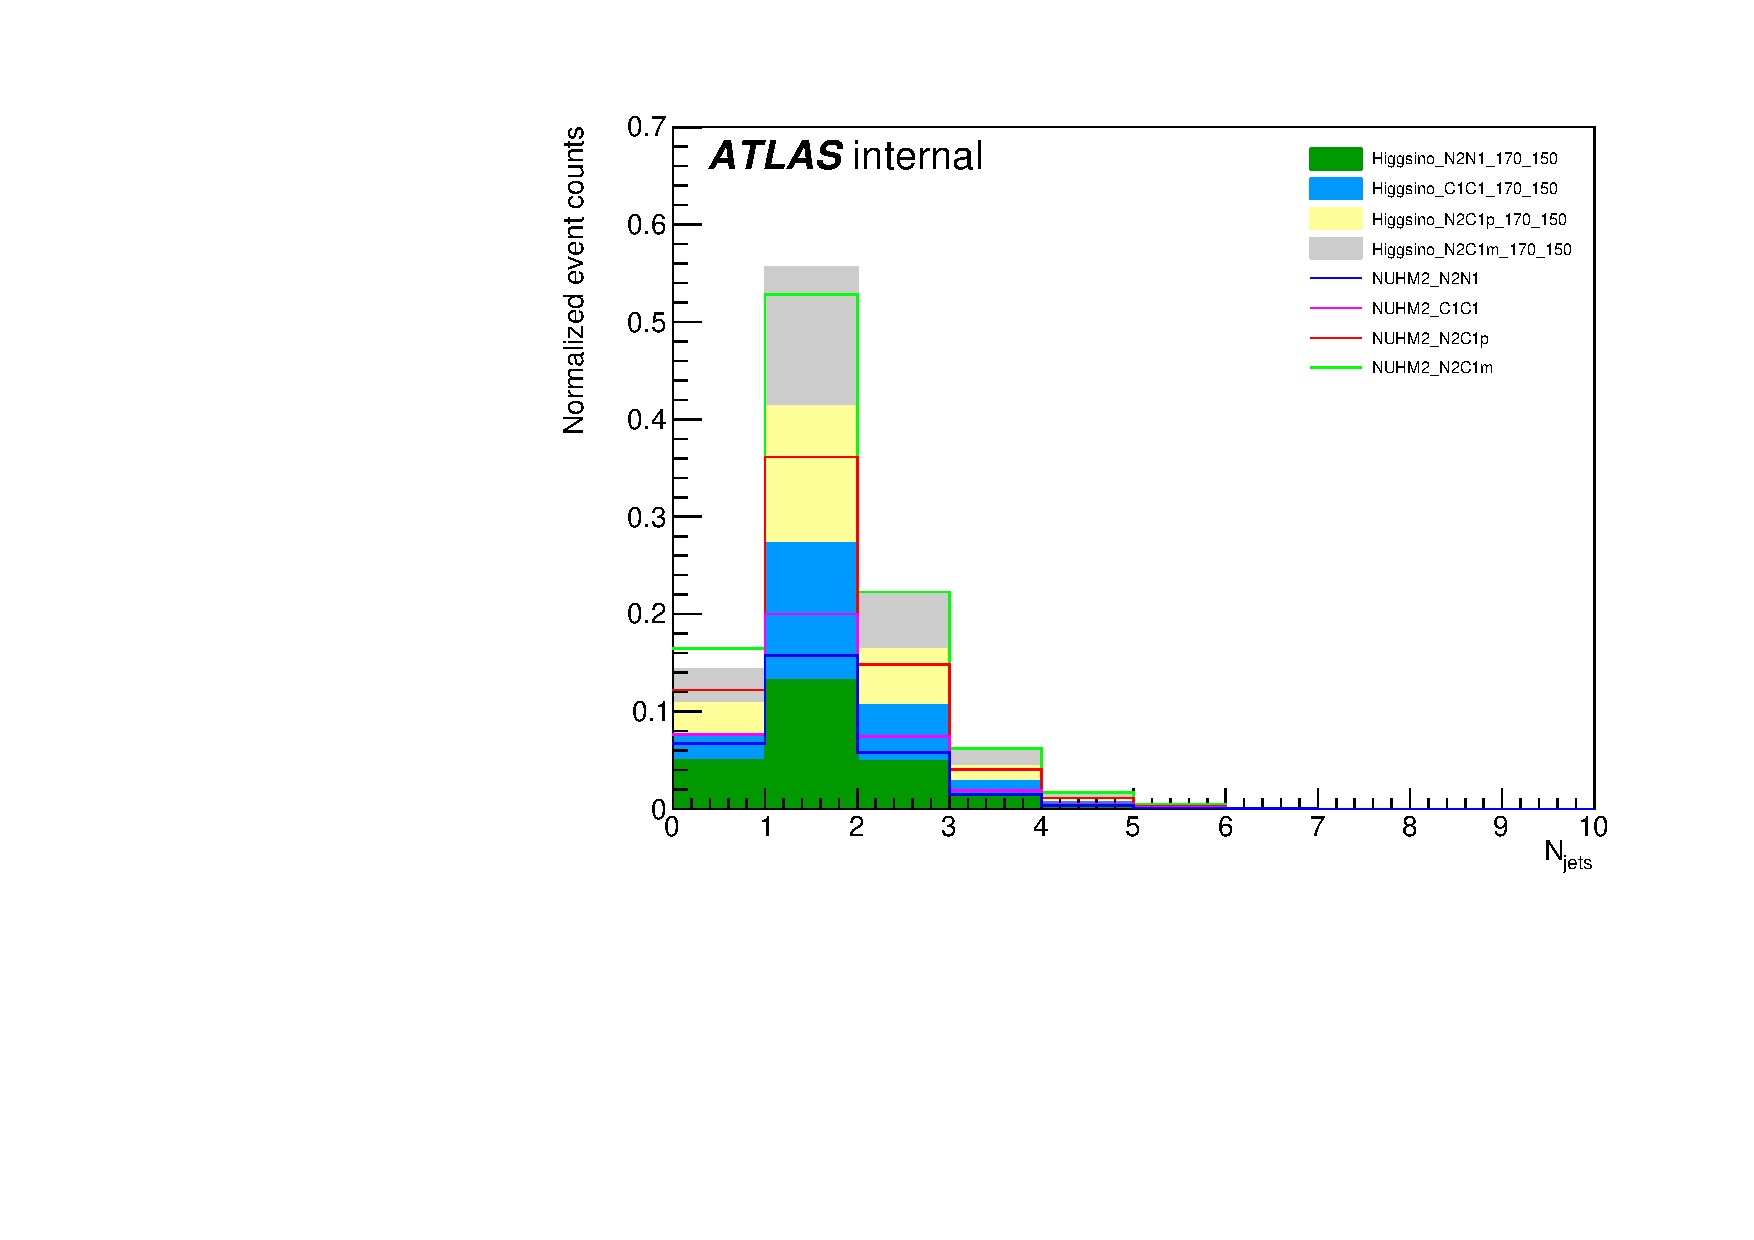
\includegraphics[scale=0.4]{nJet25.pdf}
%             \caption{Signal jets multiplicity with $\pt > 25$~{\GeV}}
%         \end{subfigure}
%         \begin{subfigure}[b]{0.48\textwidth}
%             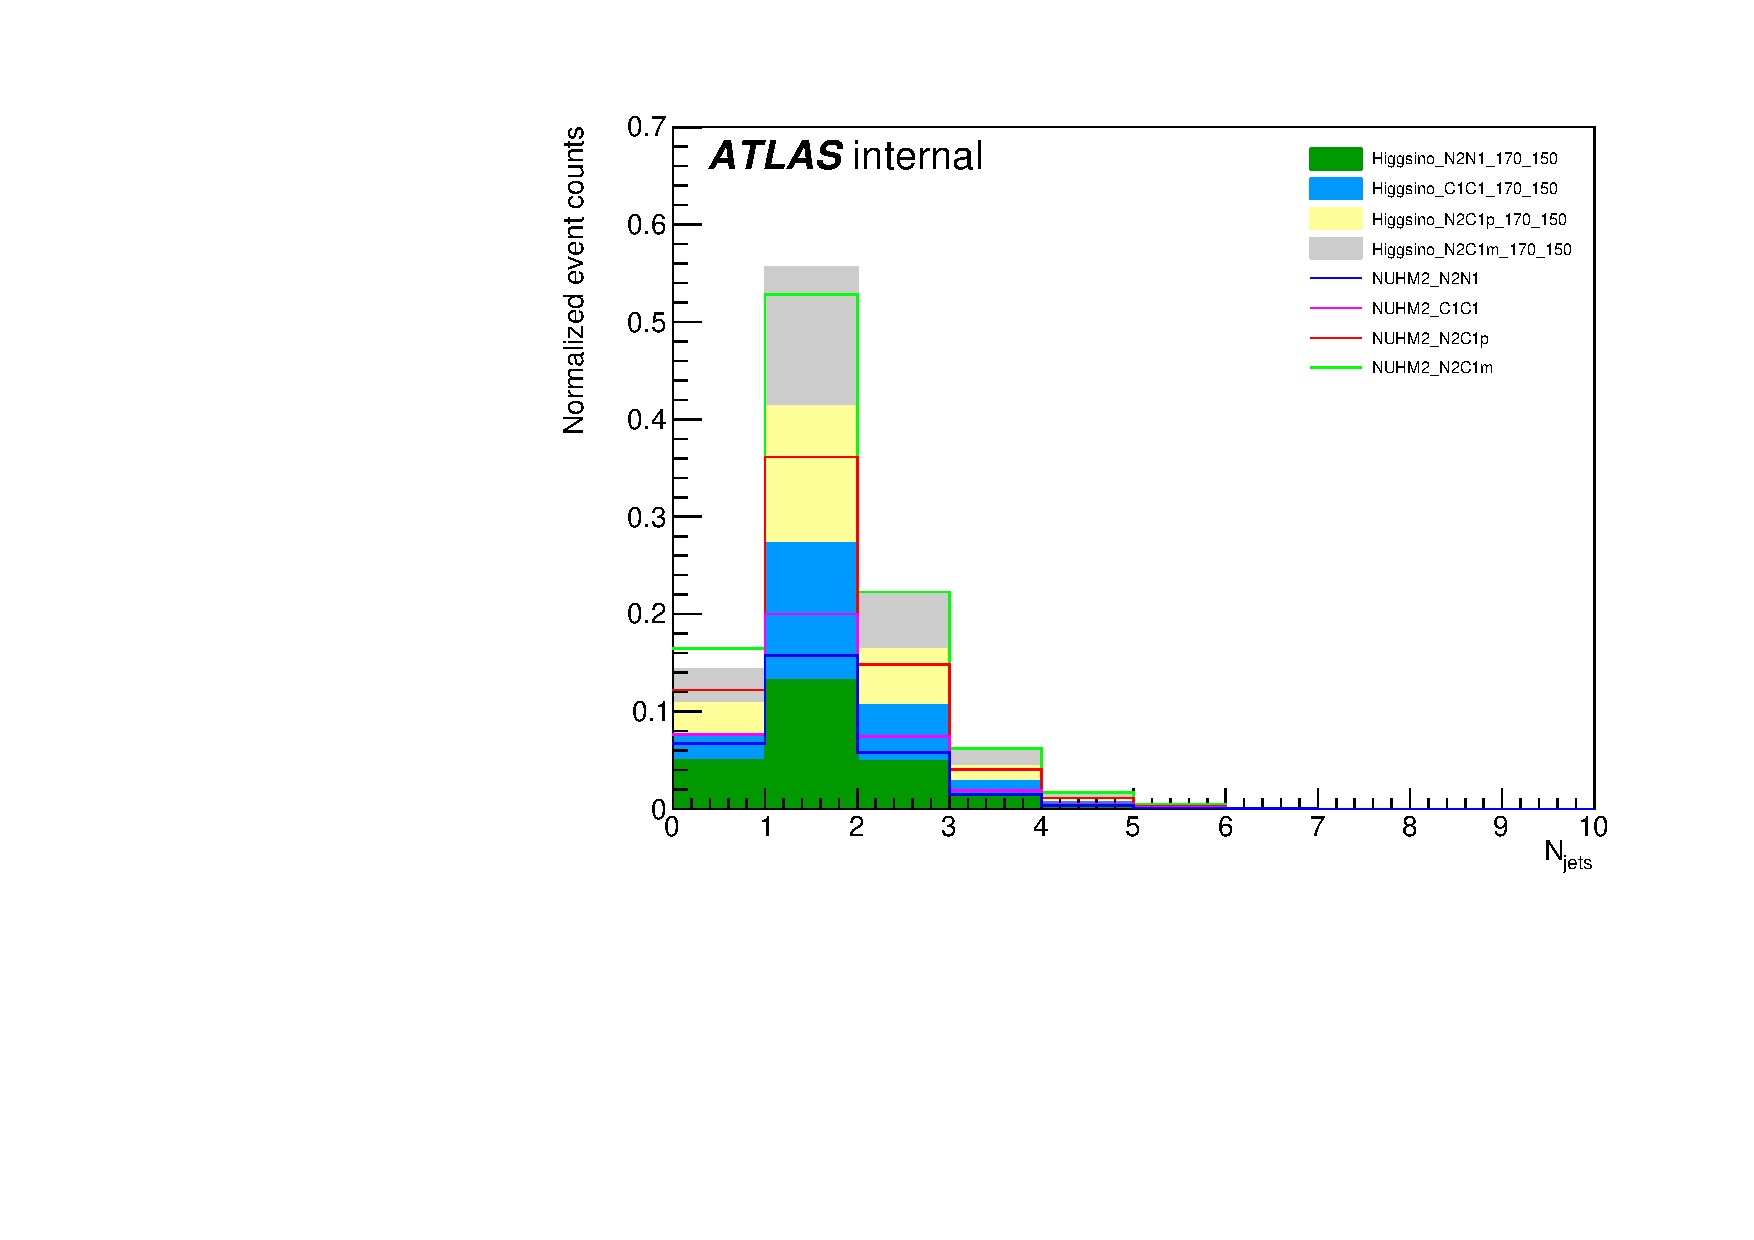
\includegraphics[scale=0.4]{nJet30.pdf}
%             \caption{Signal jets multiplicity with $\pt > 30$~{\GeV}}
%         \end{subfigure}
%     \end{center}
%     \caption{The jets multiplicity distributions.
%     The jet multiplicity of NUHM2 with $m_{1/2} = 600$~{\GeV} are compared to the simplified Higgsino model with $m_{\widetilde{\chi}^{0}_{2}}=170$~{\GeV} and $m_{\widetilde{\chi}^{0}_{1}}=150$~{\GeV}.
%     The top left plot includes the forward jets and the bottom two plots use the signal jets with $\pt > 25$~{\GeV} and $\pt > 30$~{\GeV}, respectively.
%     Four different production channels, $\widetilde{\chi}^{0}_{2}\widetilde{\chi}^{0}_{1}$, $\widetilde{\chi}^{0}_{2}\widetilde{\chi}^{+}_{1}$, $\widetilde{\chi}^{0}_{2}\widetilde{\chi}^{-}_{1}$, and $\widetilde{\chi}^{\pm}_{1}\widetilde{\chi}^{\mp}_{1}$, for the NUHM2 and the simplified Higgsino model are considered.
%     The distributions of four productions are combined and normalized to equal area.}
%     \label{fig:results_nuhm2_jets_multiplicity}
% \end{figure}

% \begin{figure}[htbp]
%     \begin{center}
%         \begin{subfigure}[b]{0.48\textwidth}
%             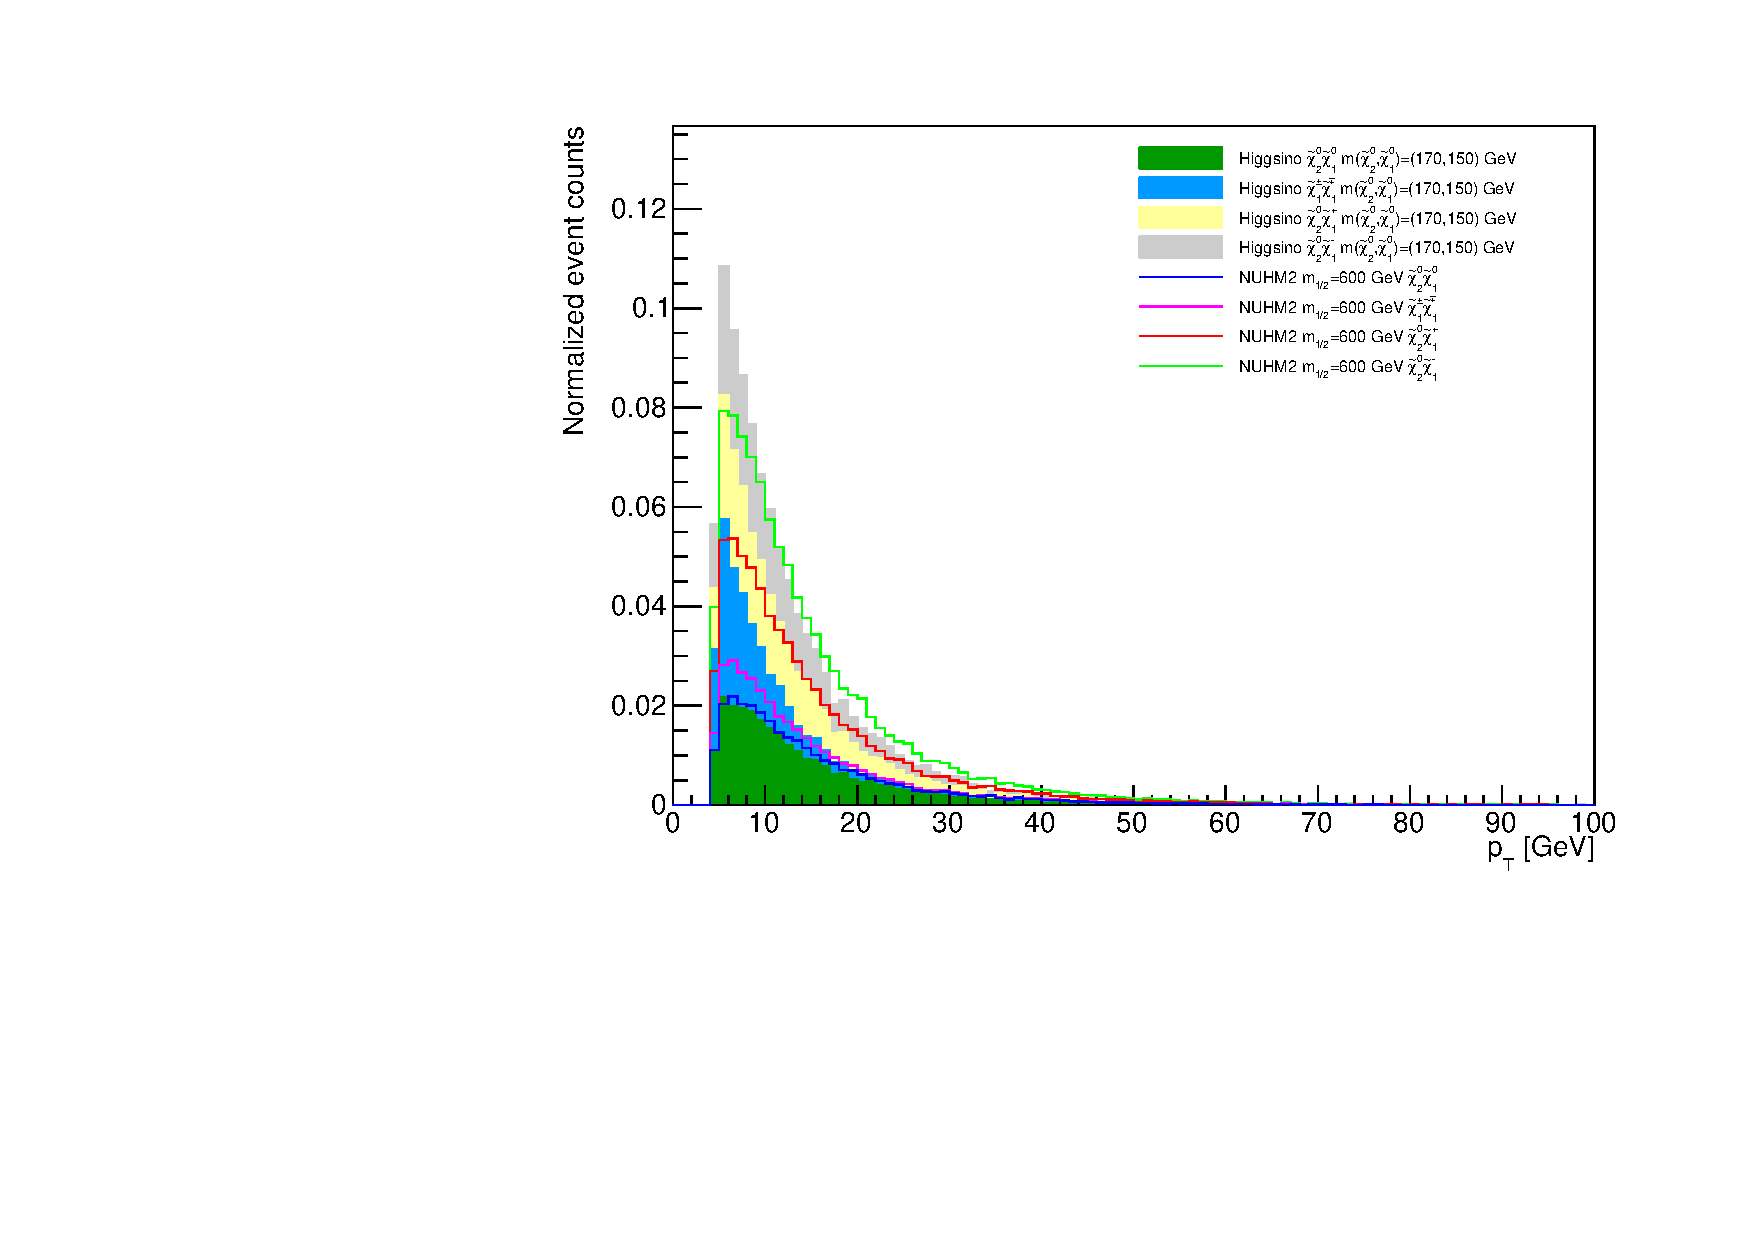
\includegraphics[scale=0.35]{signalElectrons_pt.pdf}
%             \caption{Signal electrons \pt}
%         \end{subfigure}
%         \begin{subfigure}[b]{0.48\textwidth}
%             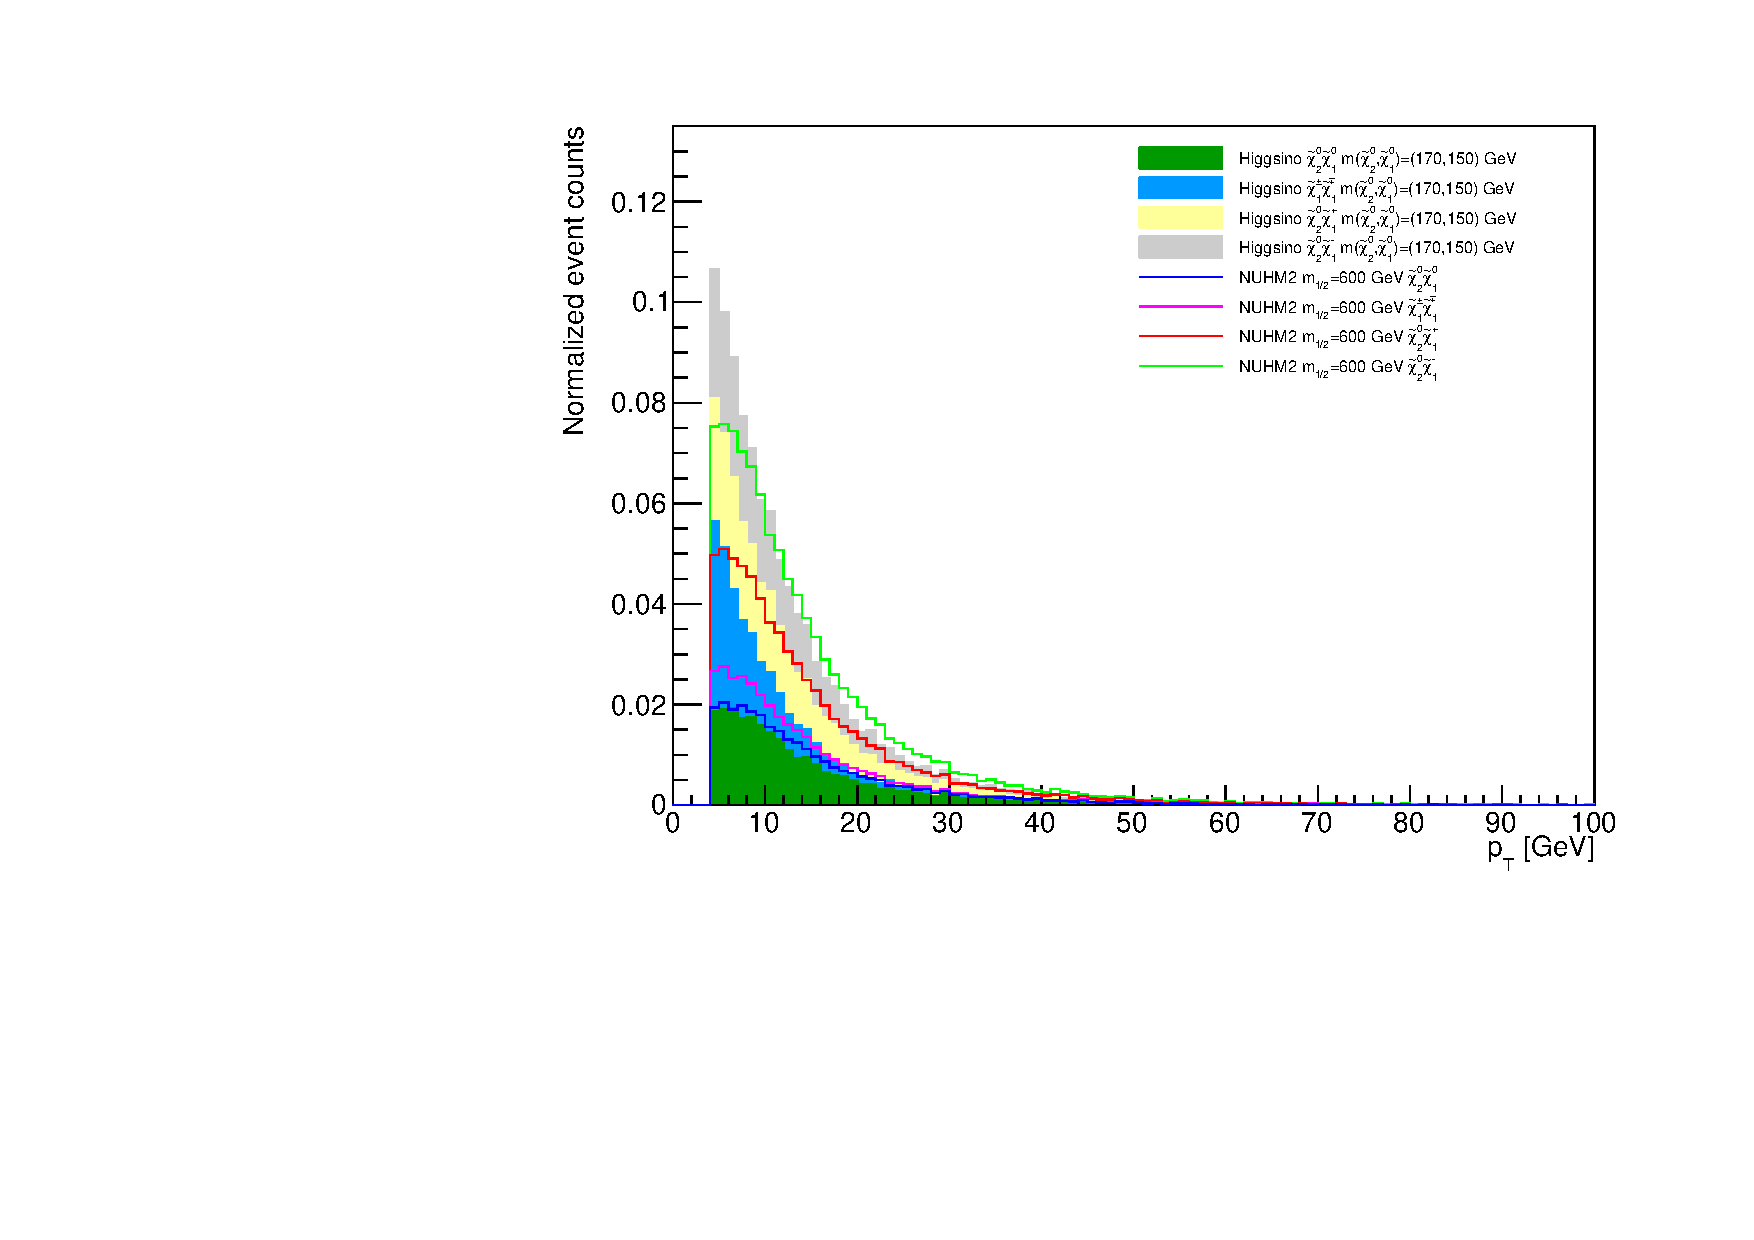
\includegraphics[scale=0.35]{signalMuons_pt.pdf}
%             \caption{Signal muons \pt}
%         \end{subfigure}
%         \begin{subfigure}[b]{0.48\textwidth}
%             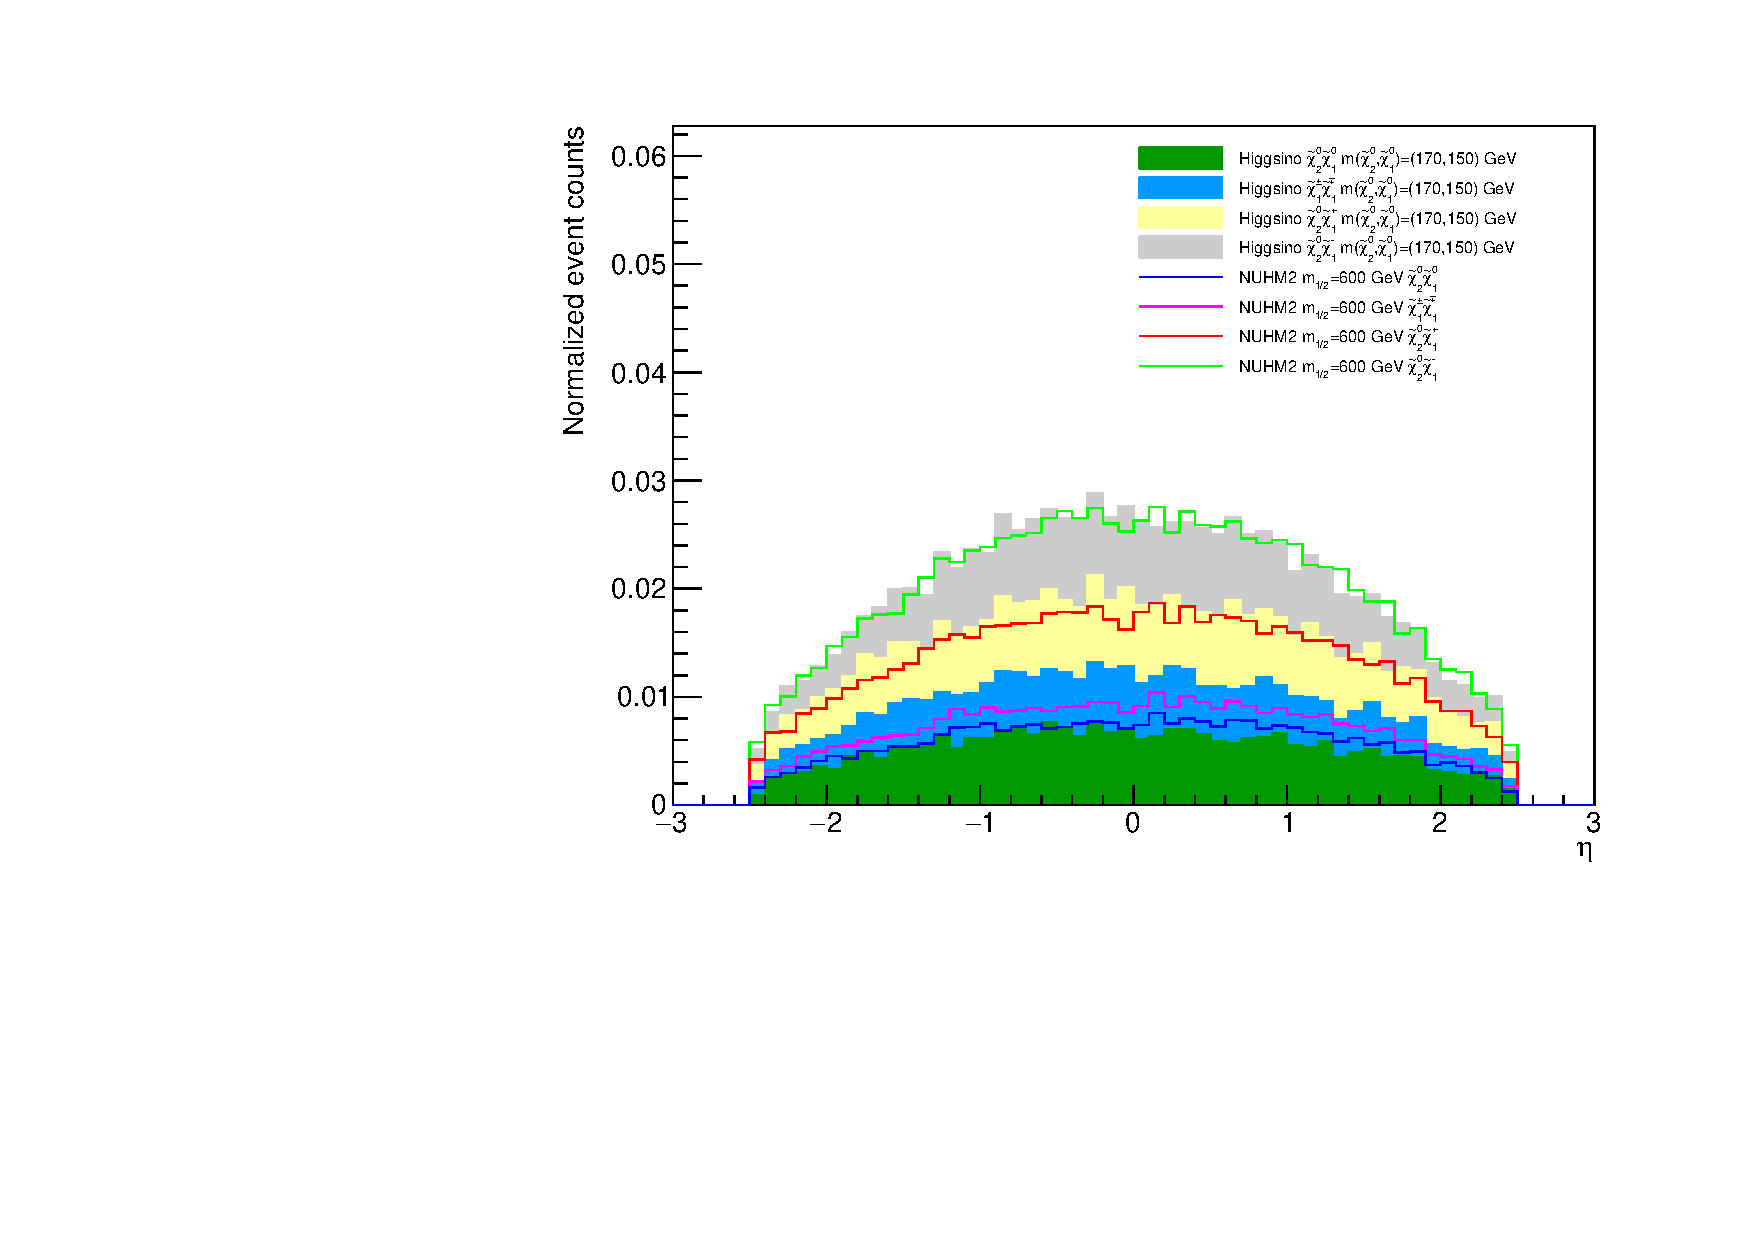
\includegraphics[scale=0.35]{signalElectrons_eta.pdf}
%             \caption{Signal electrons $\eta$}
%         \end{subfigure}
%         \begin{subfigure}[b]{0.48\textwidth}
%             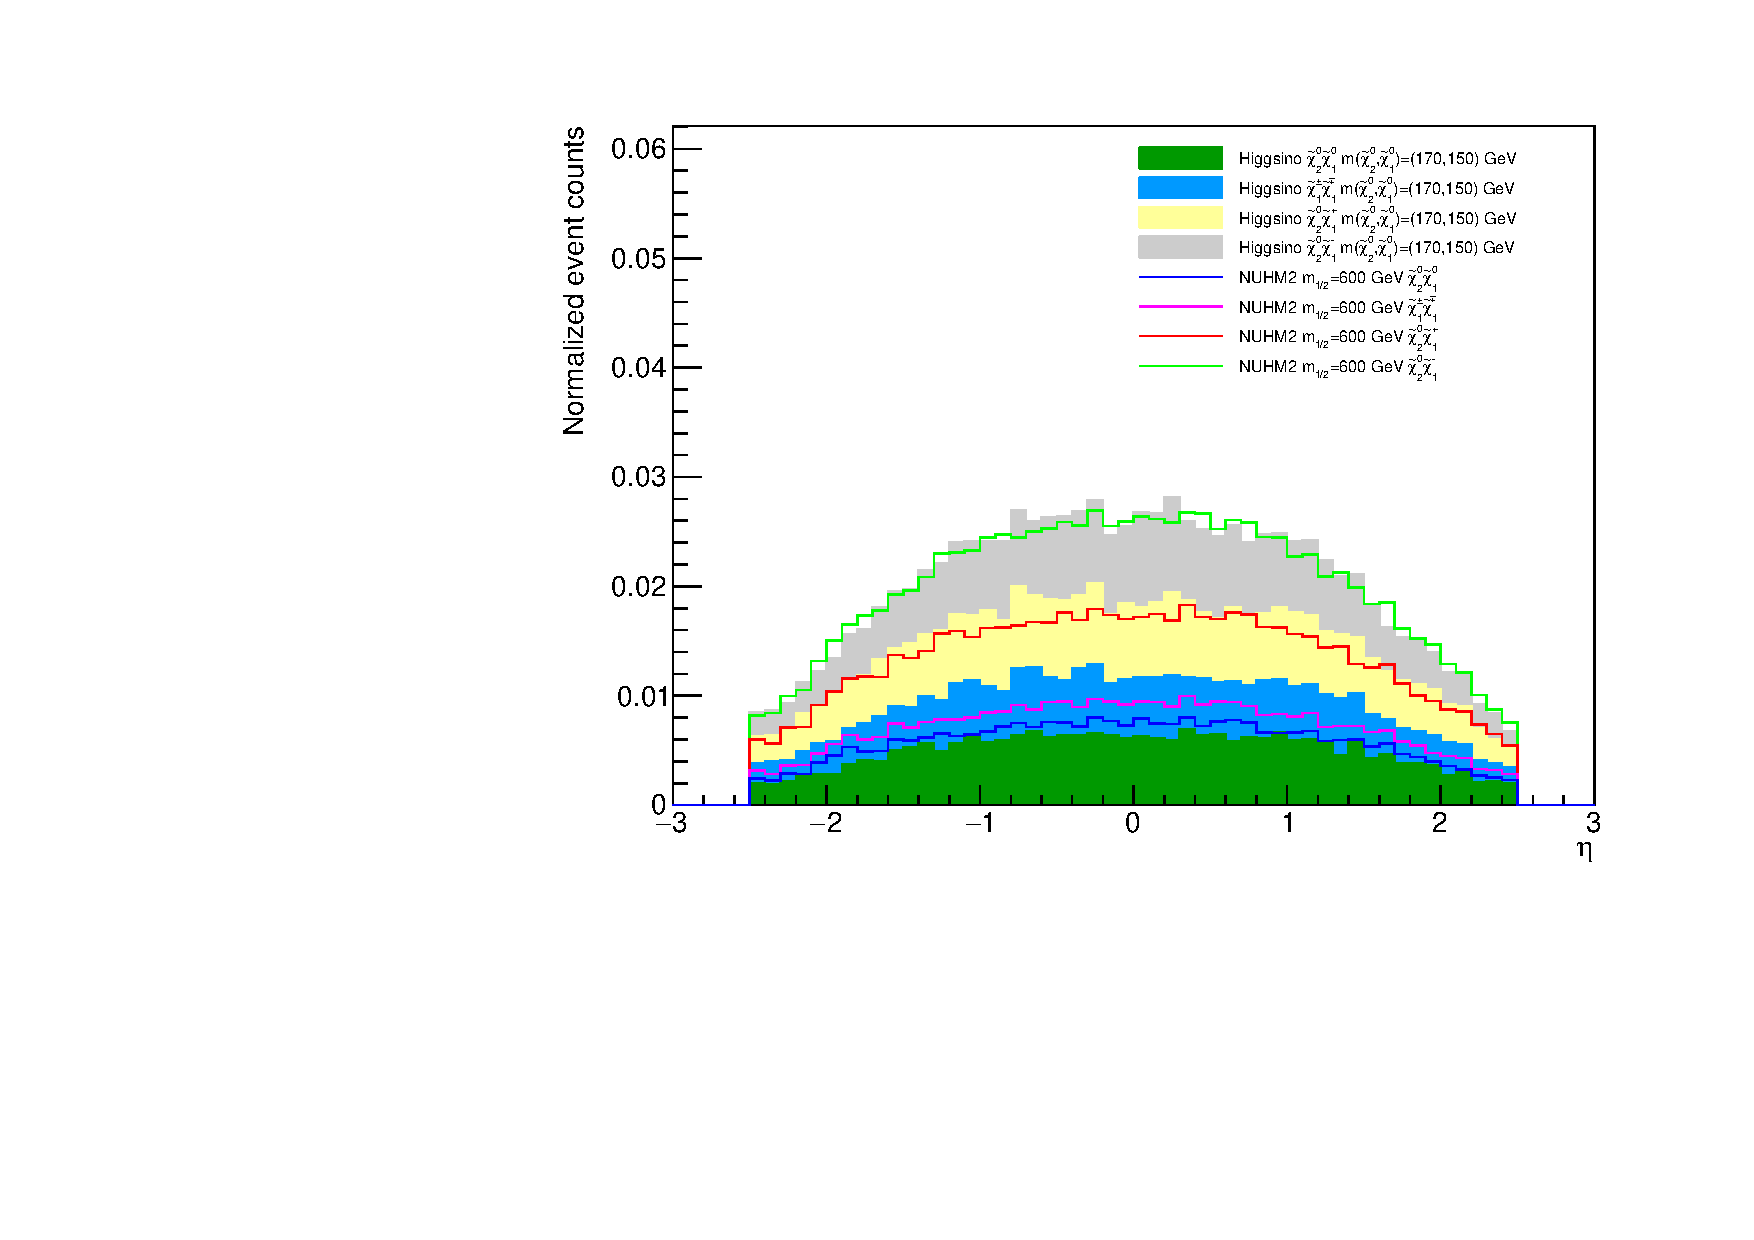
\includegraphics[scale=0.35]{signalMuons_eta.pdf}
%             \caption{Signal muons $\eta$}
%         \end{subfigure}
%         \begin{subfigure}[b]{0.48\textwidth}
%             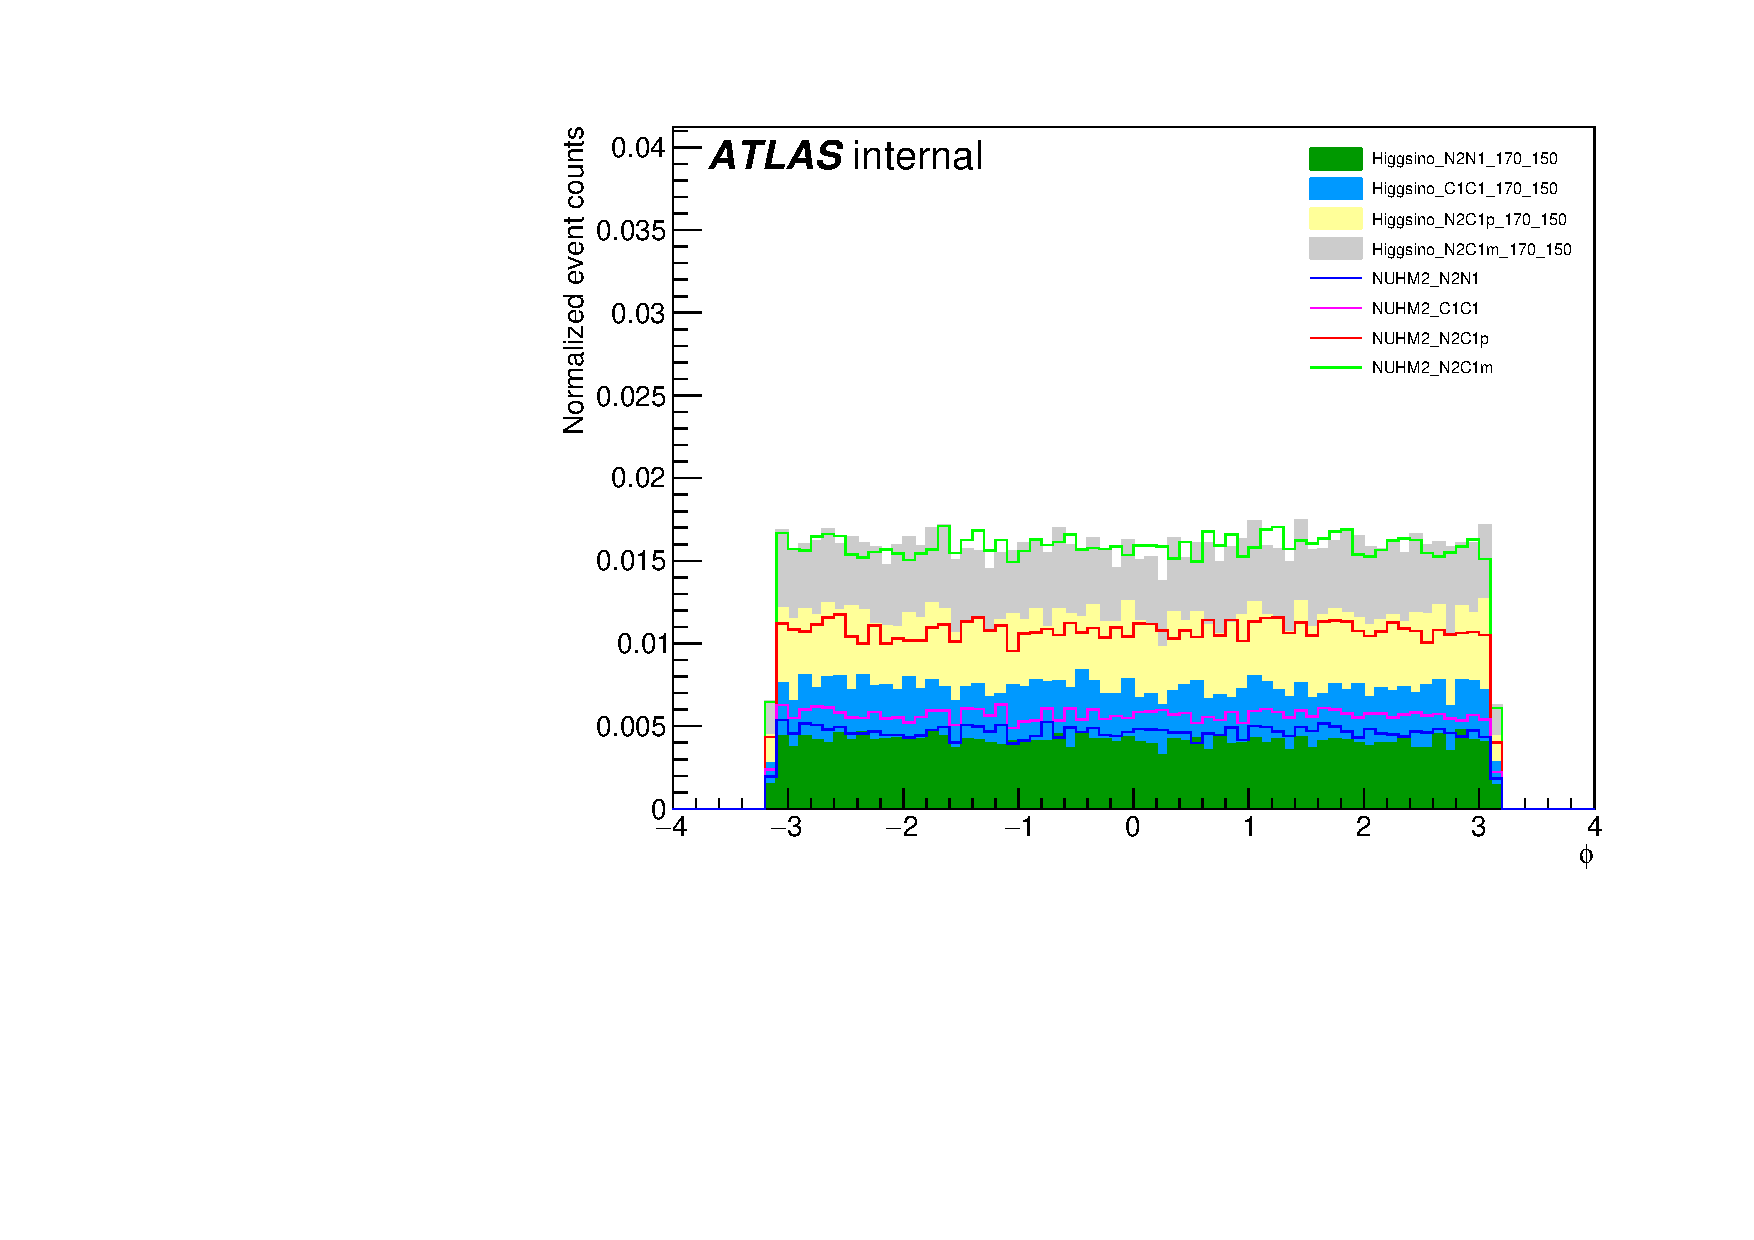
\includegraphics[scale=0.35]{signalElectrons_phi.pdf}
%             \caption{Signal electrons $\phi$}
%         \end{subfigure}
%         \begin{subfigure}[b]{0.48\textwidth}
%             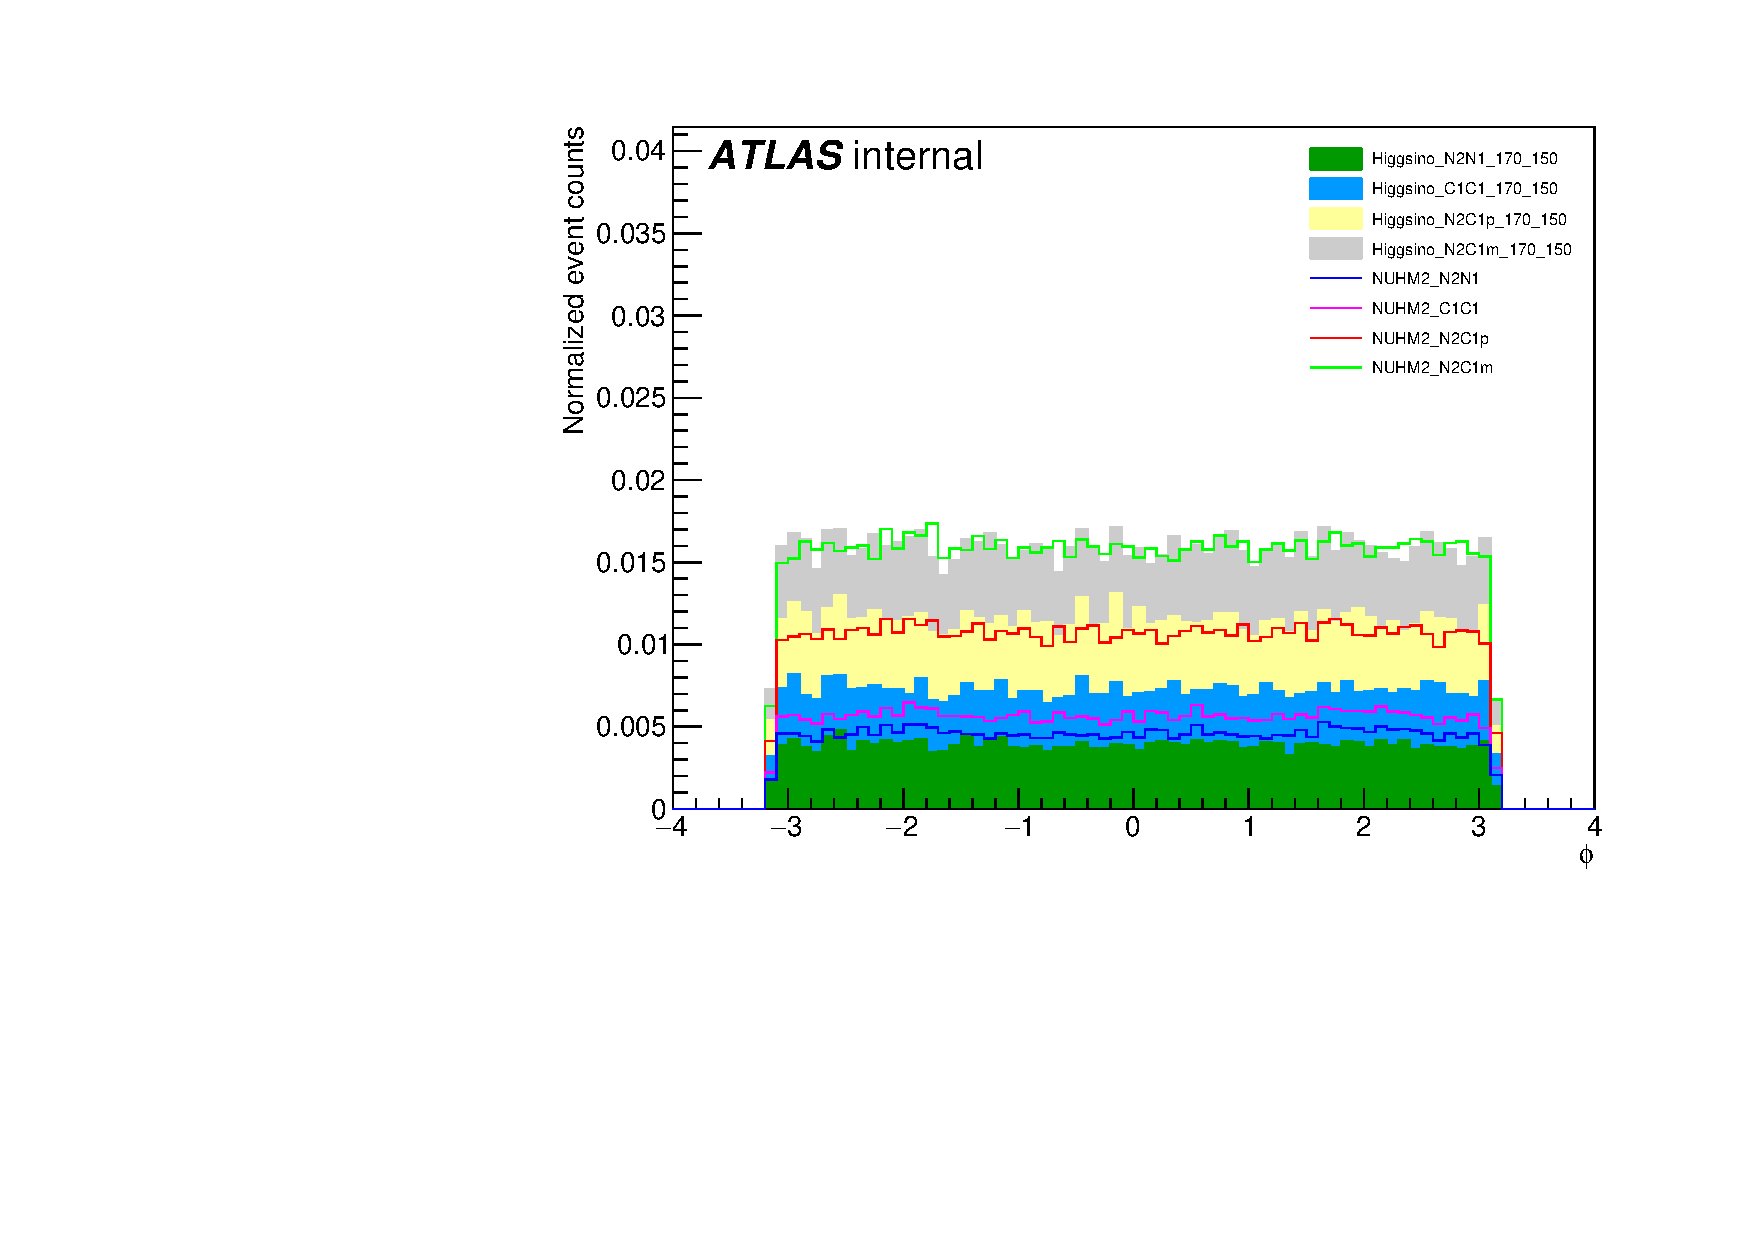
\includegraphics[scale=0.35]{signalMuons_phi.pdf}
%             \caption{Signal muons $\phi$}
%         \end{subfigure}
%     \end{center}
%     \caption{The \pt, $\eta$, and $\phi$ distributions for the NUHM2 with $m_{1/2} = 600$~{\GeV} and the simplified Higgsino model with $m_{\widetilde{\chi}^{0}_{2}}=170$~{\GeV} and $m_{\widetilde{\chi}^{0}_{1}}=150$~{\GeV}.
%     The signal electrons \pt, $\eta$, and $\phi$ distributions are on the left column and the signal muons distributions are on the right.
%     Four different production channels, $\widetilde{\chi}^{0}_{2}\widetilde{\chi}^{0}_{1}$, $\widetilde{\chi}^{0}_{2}\widetilde{\chi}^{+}_{1}$, $\widetilde{\chi}^{0}_{2}\widetilde{\chi}^{-}_{1}$, and $\widetilde{\chi}^{\pm}_{1}\widetilde{\chi}^{\mp}_{1}$, for the NUHM2 and the simplified Higgsino model are considered.
%     The distributions of four productions are combined and normalized to equal area.}
%     \label{fig:results_nuhm2_leptons_pt_eta_phi}
% \end{figure}

% \begin{figure}[htbp]
%     \begin{center}
%         \begin{subfigure}[b]{0.48\textwidth}
%             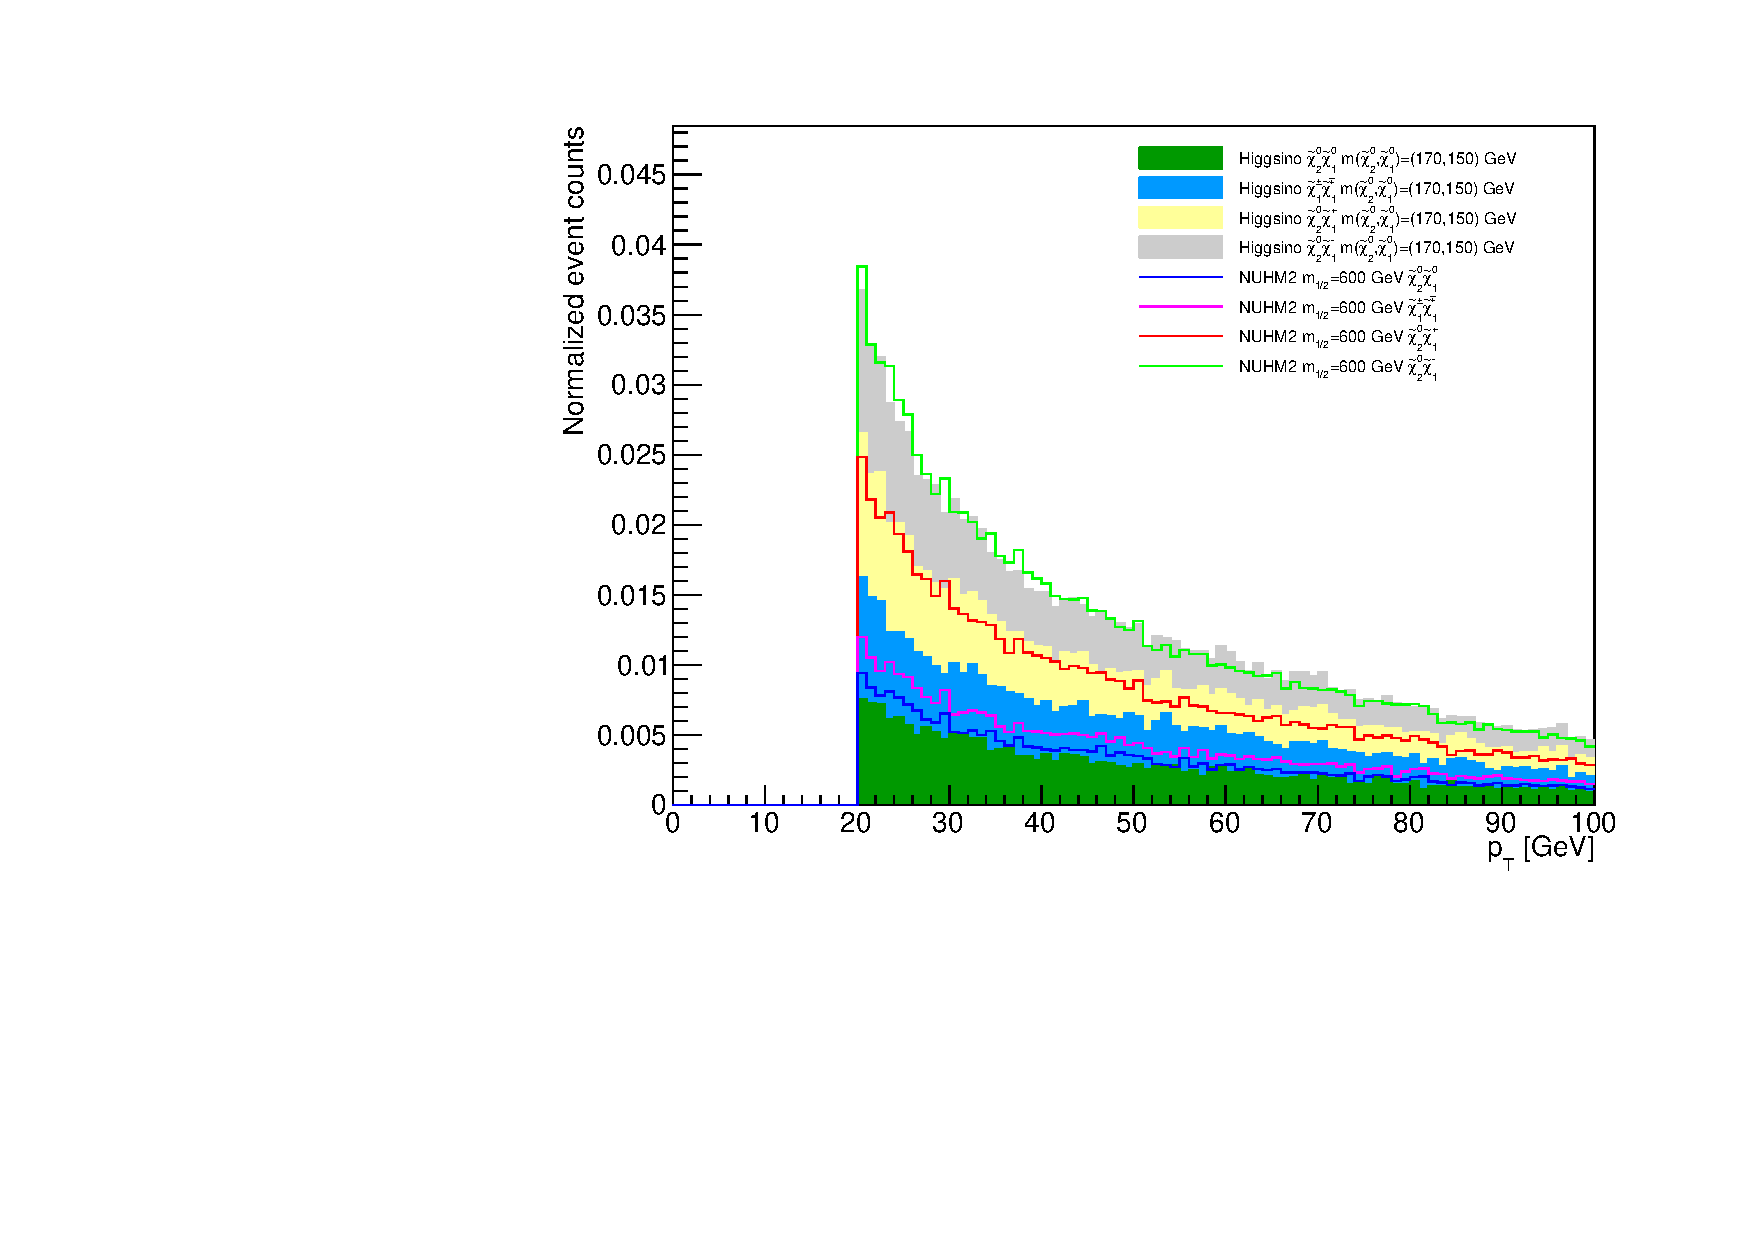
\includegraphics[scale=0.35]{signalJets_pt.pdf}
%             \caption{The signal jets \pt.}
%         \end{subfigure}
%         \begin{subfigure}[b]{0.48\textwidth}
%             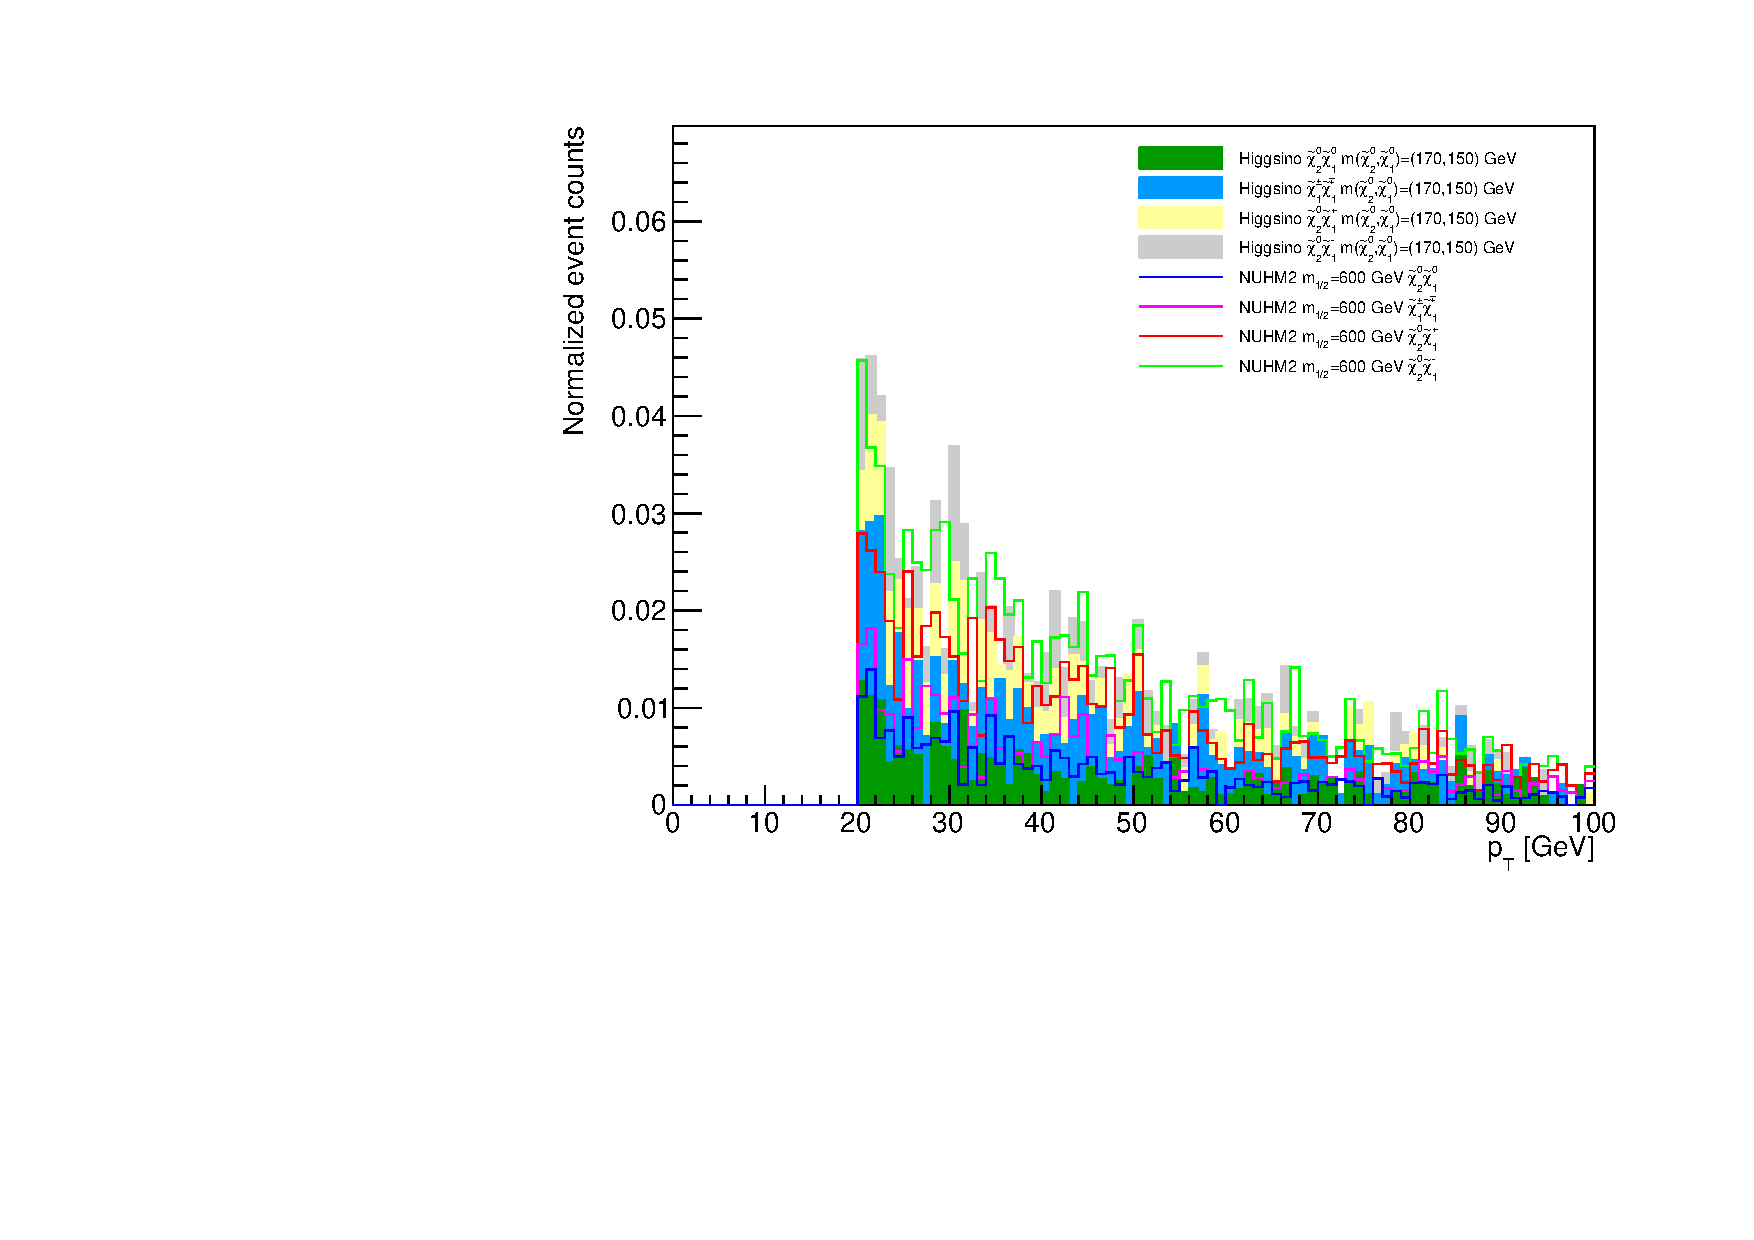
\includegraphics[scale=0.35]{signalBjets_pt.pdf}
%             \caption{The signal $b$-jets \pt.}
%         \end{subfigure}
%         \begin{subfigure}[b]{0.48\textwidth}
%             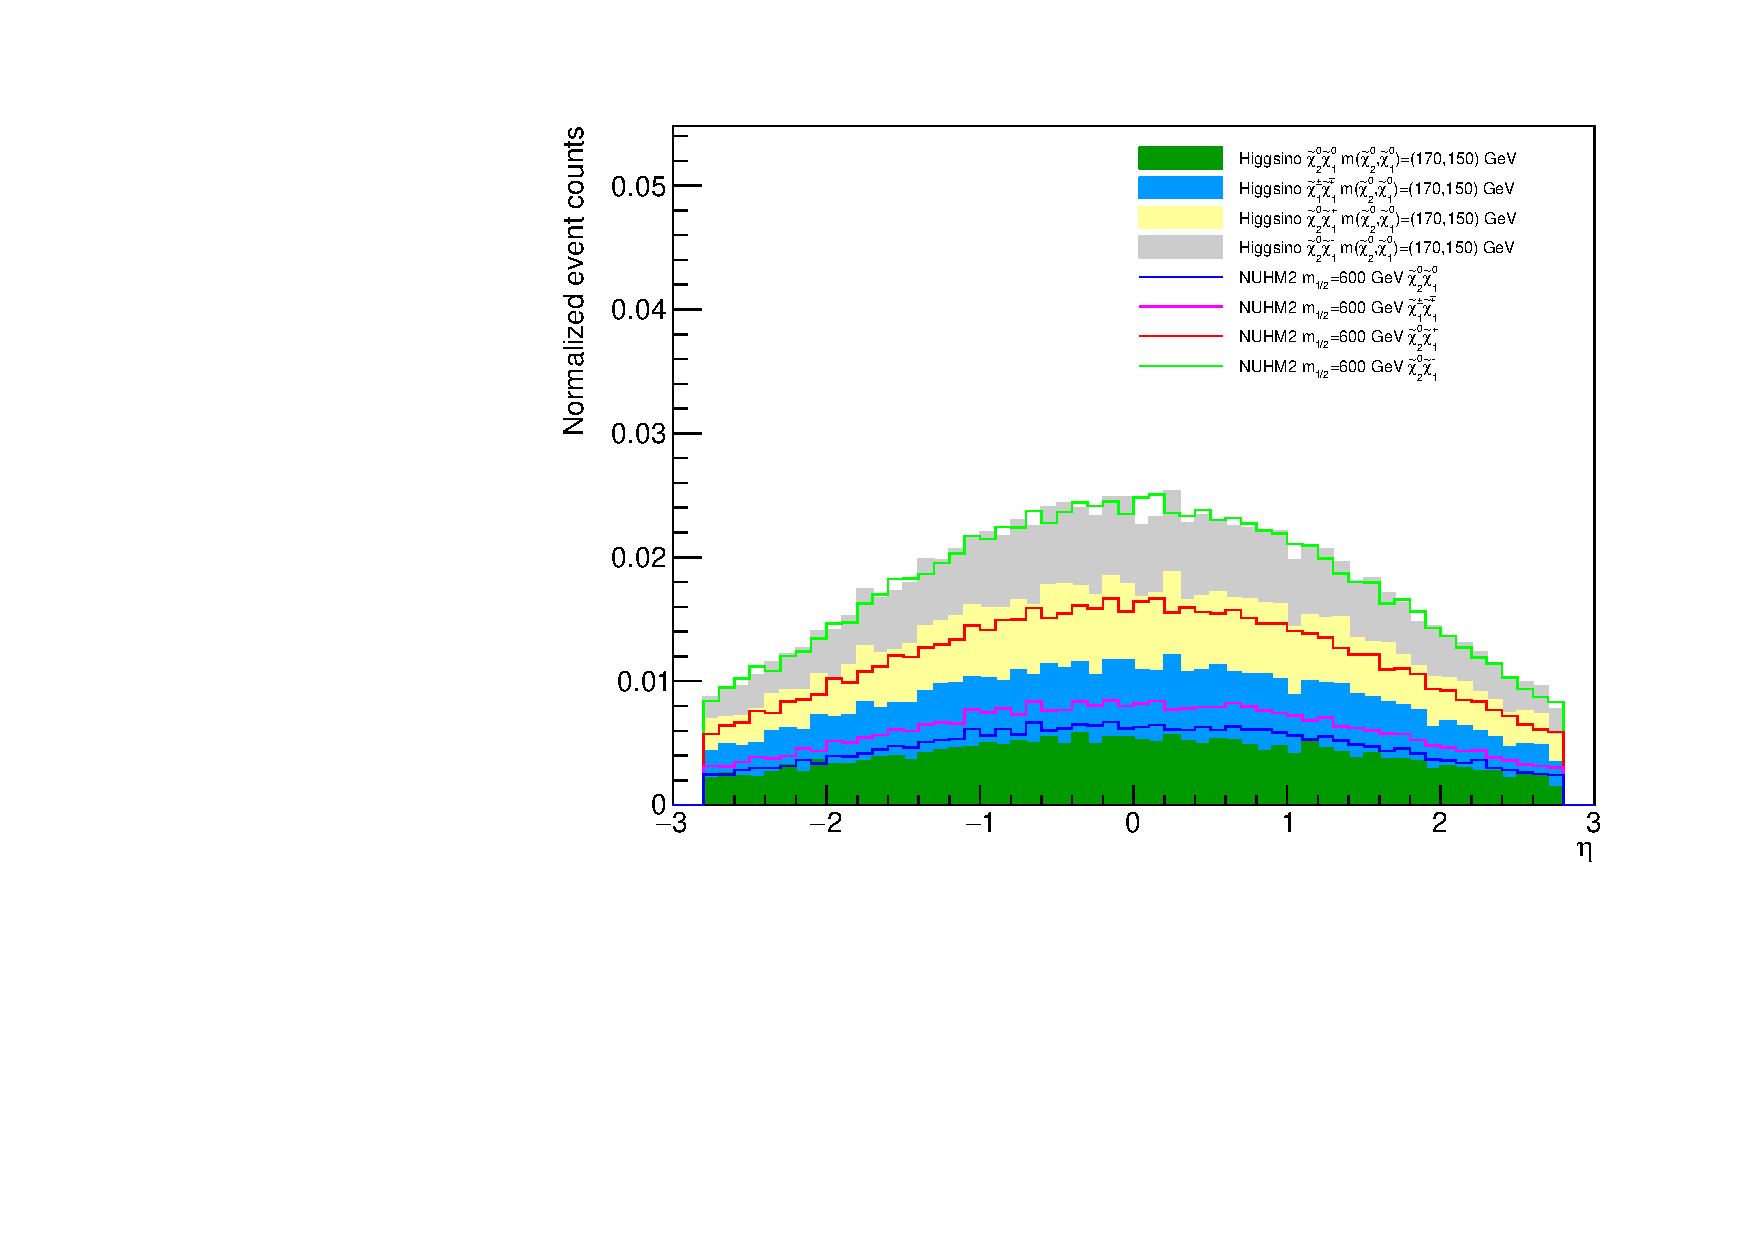
\includegraphics[scale=0.35]{signalJets_eta.pdf}
%             \caption{The signal jets $\eta$.}
%         \end{subfigure}
%         \begin{subfigure}[b]{0.48\textwidth}
%             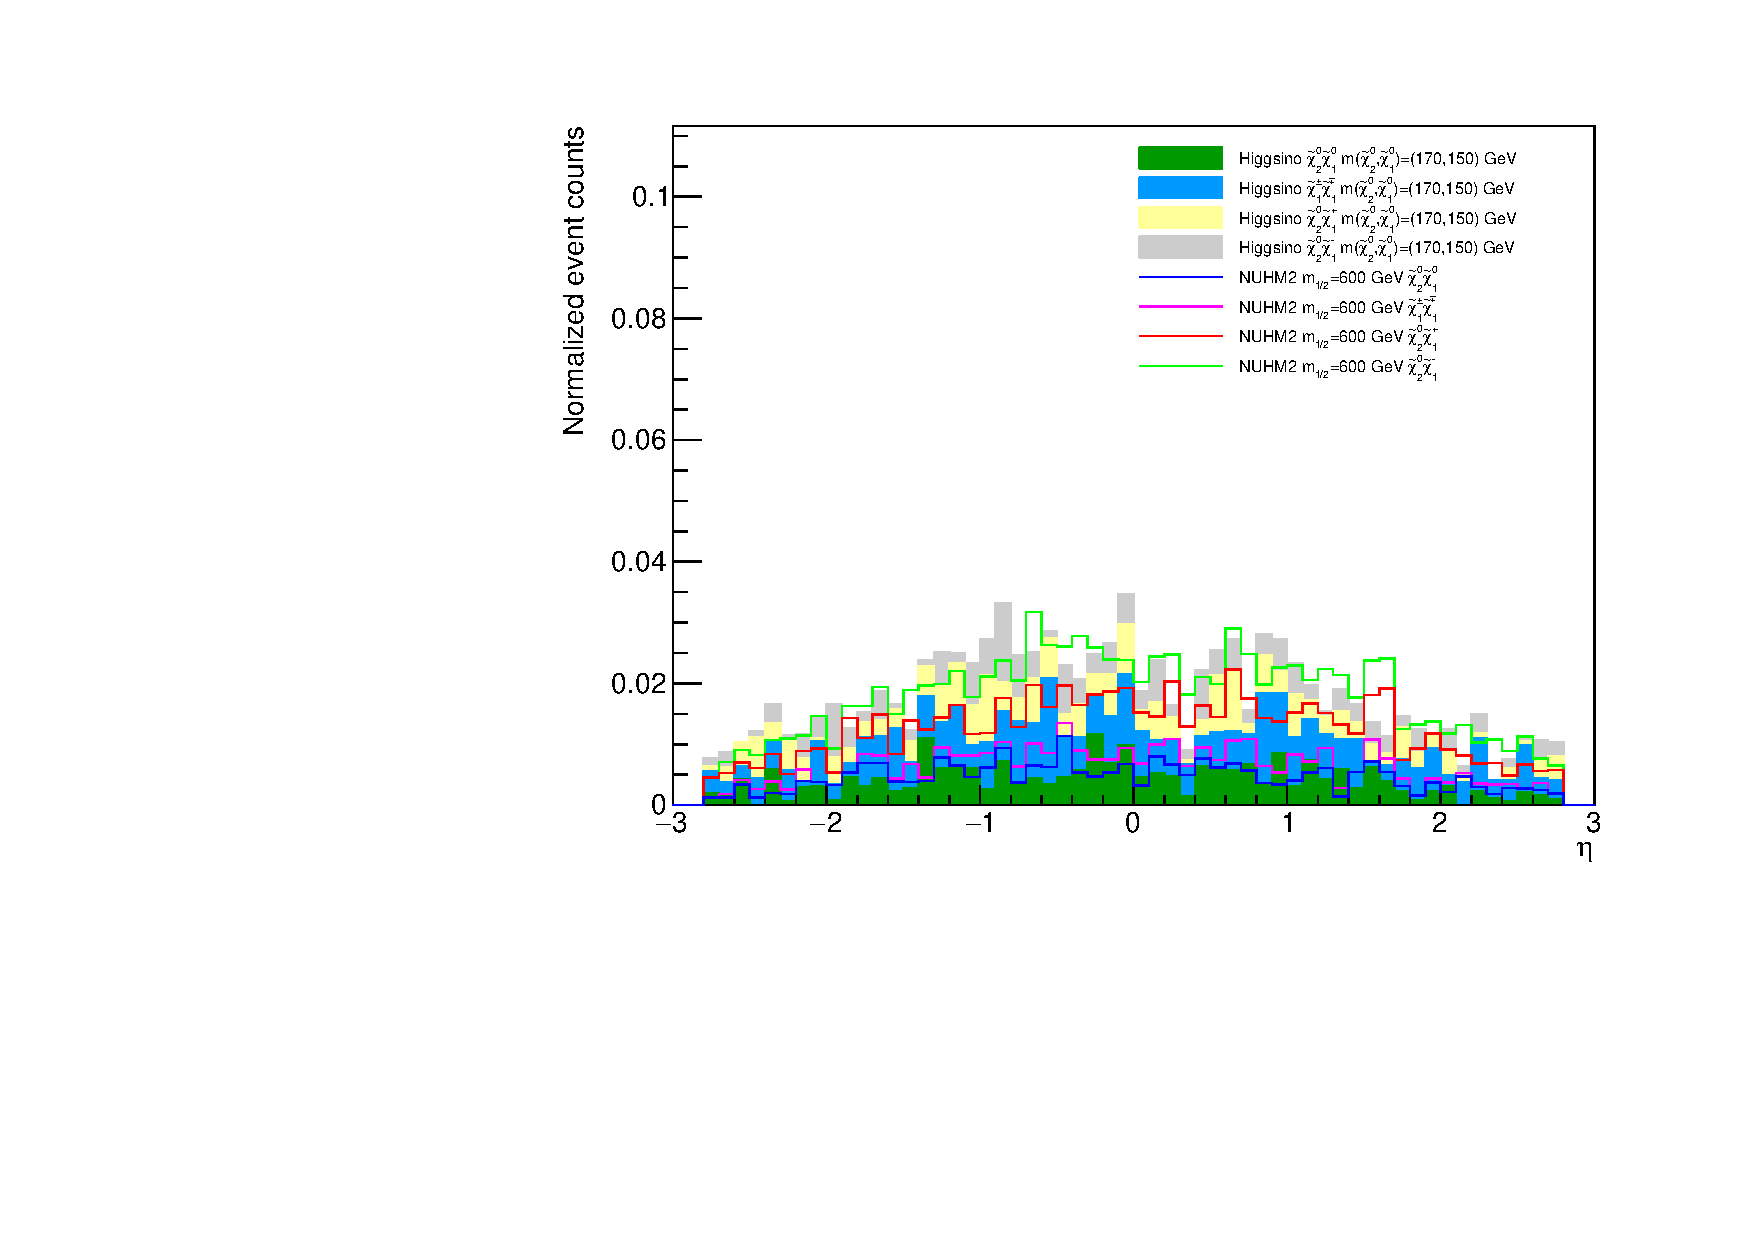
\includegraphics[scale=0.35]{signalBjets_eta.pdf}
%             \caption{The signal $b$-jets $\eta$.}
%         \end{subfigure}
%         \begin{subfigure}[b]{0.48\textwidth}
%             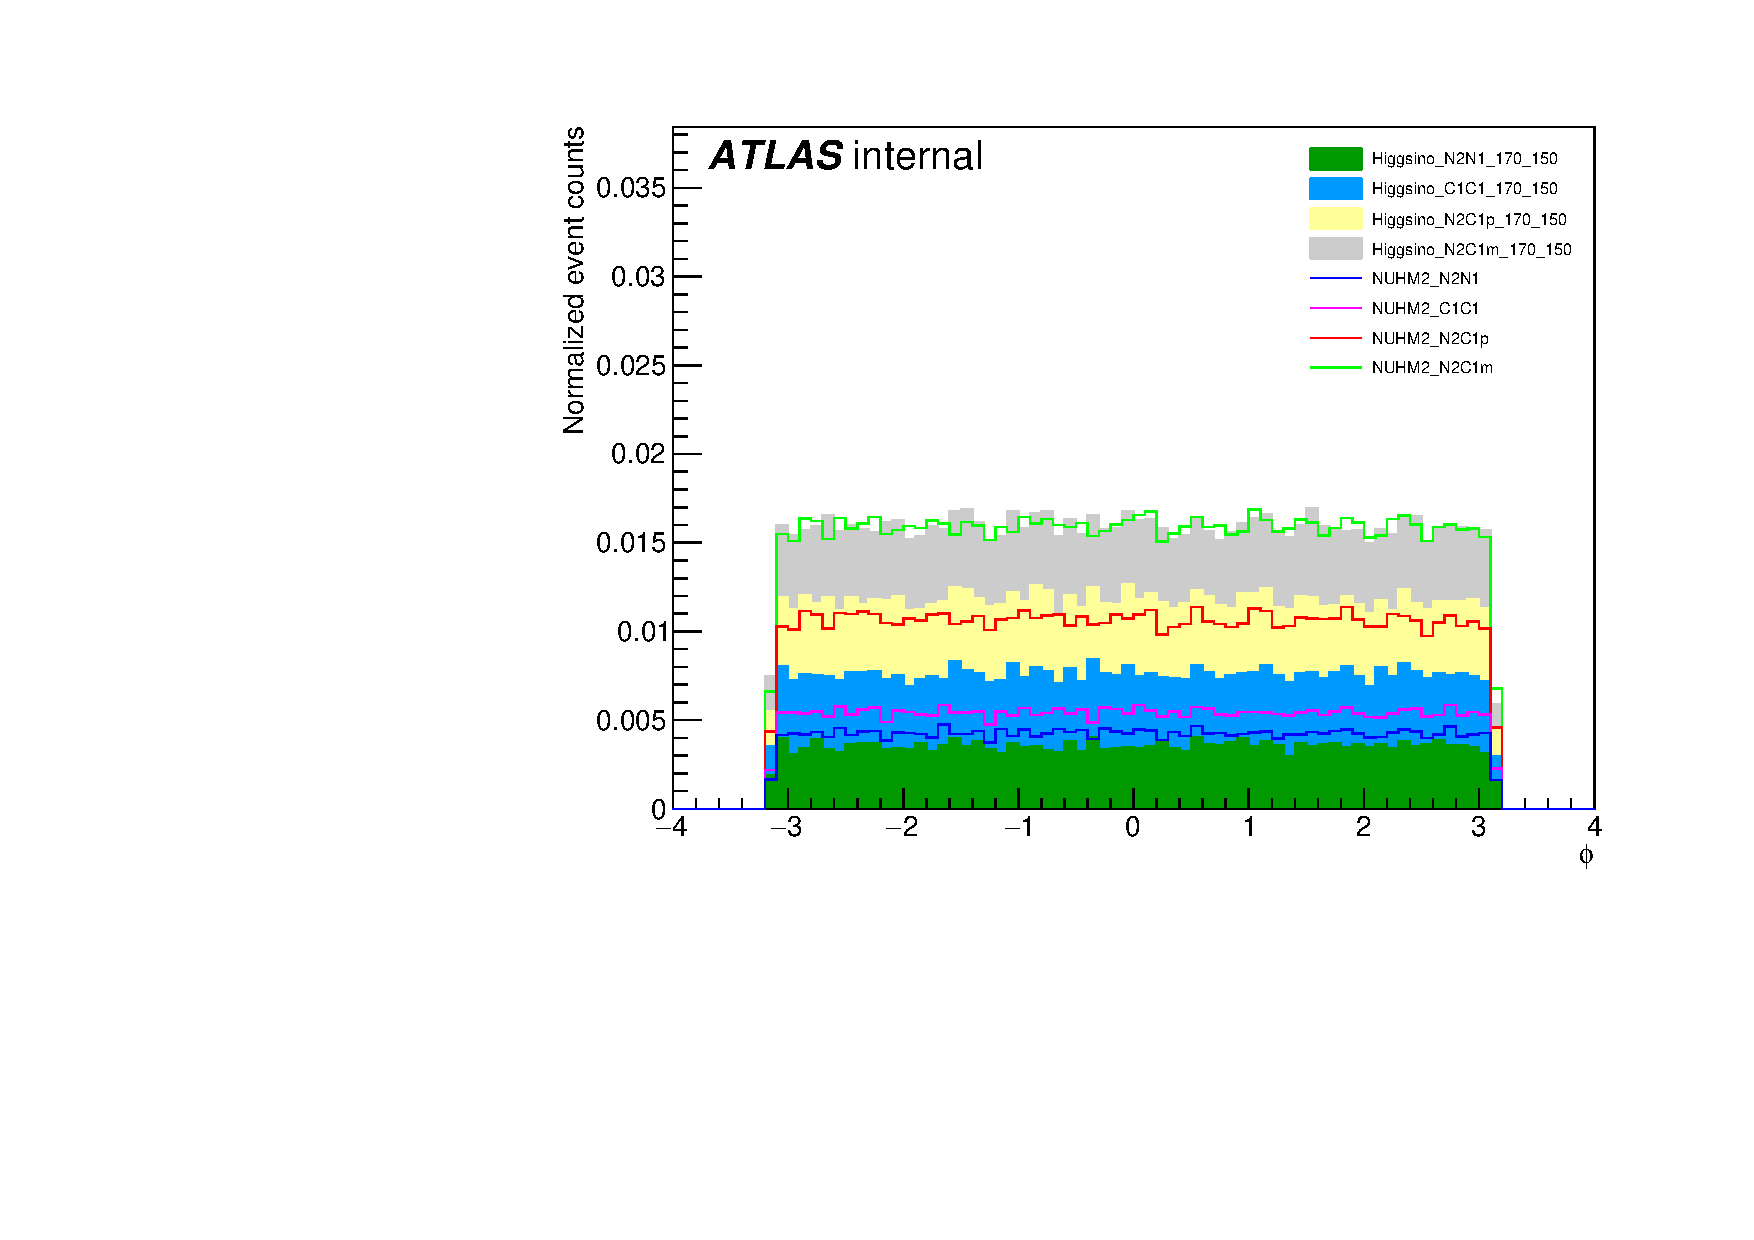
\includegraphics[scale=0.35]{signalJets_phi.pdf}
%             \caption{The signal jets $\phi$.}
%         \end{subfigure}
%         \begin{subfigure}[b]{0.48\textwidth}
%             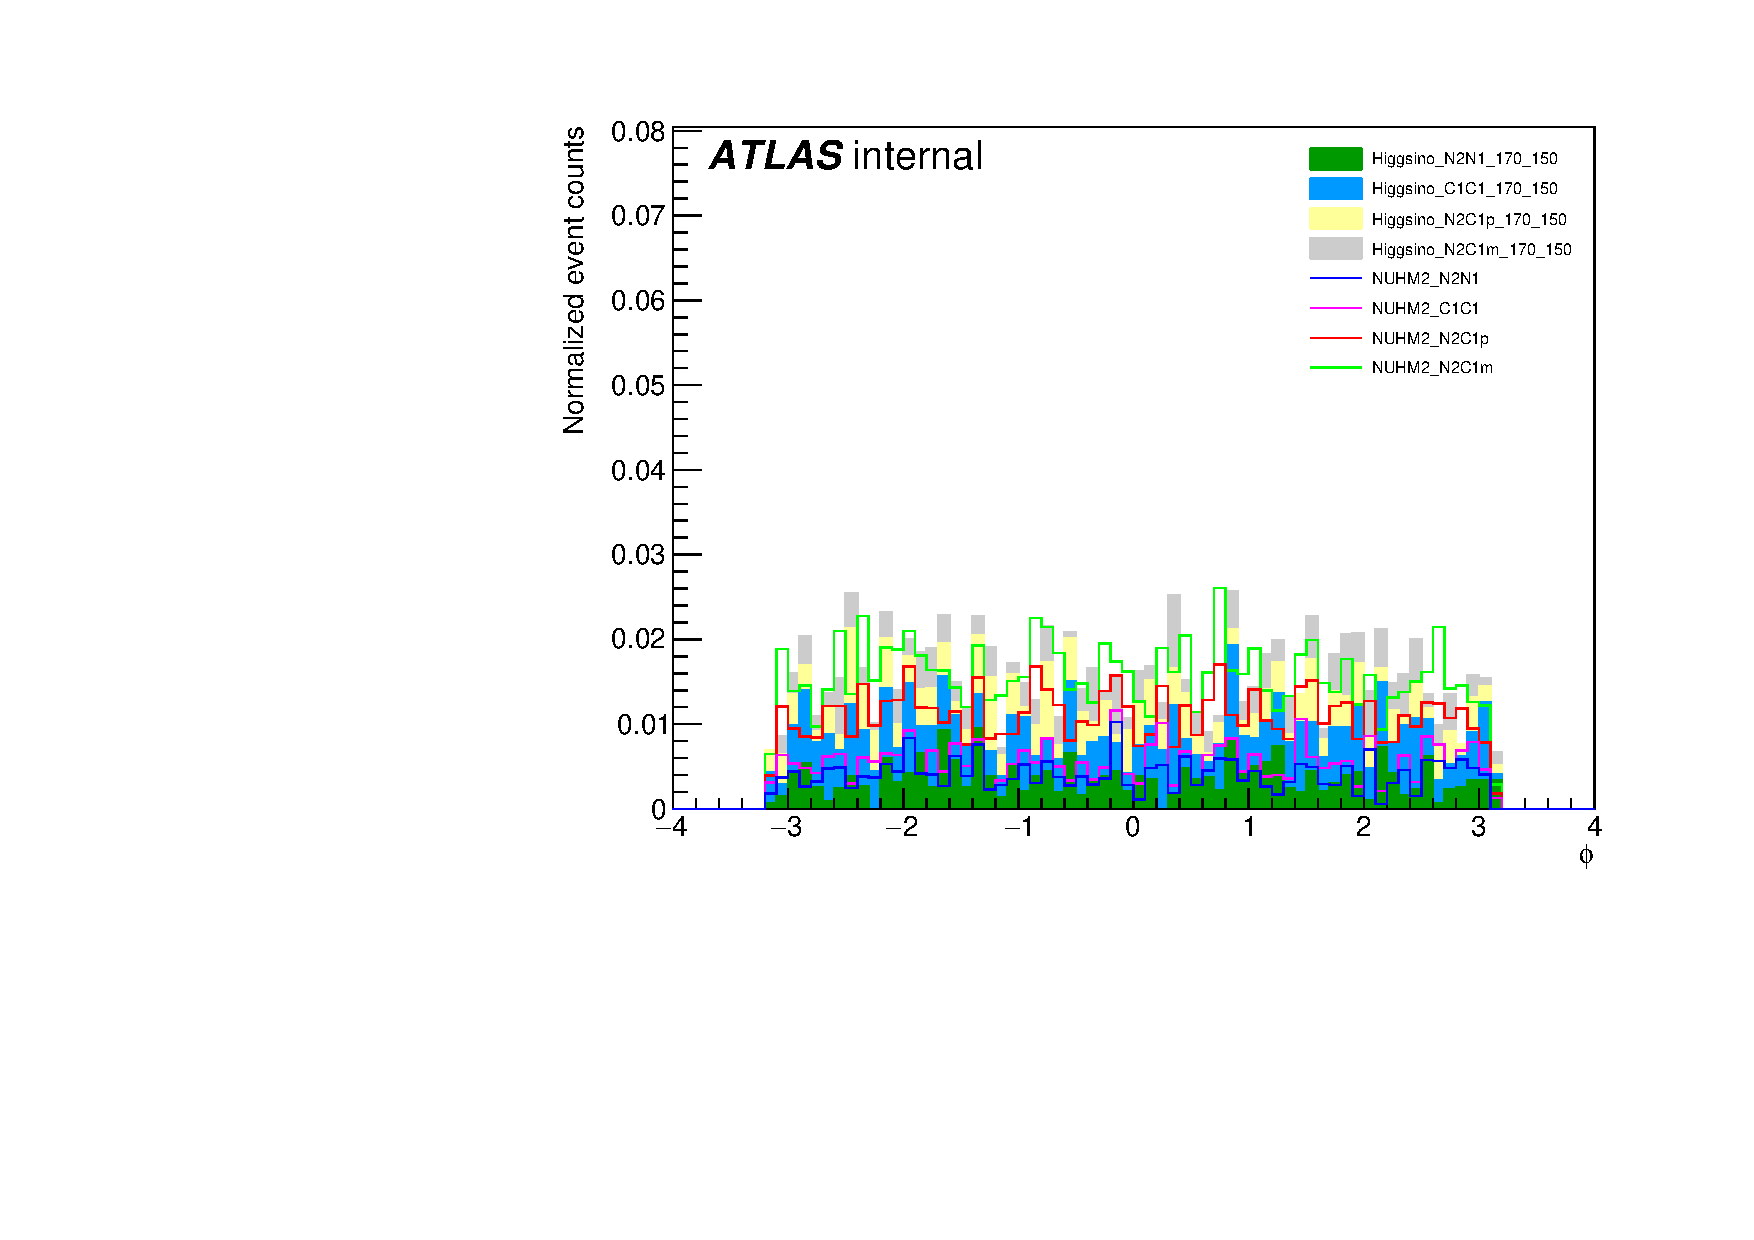
\includegraphics[scale=0.35]{signalBjets_phi.pdf}
%             \caption{The signal $b$-jets $\phi$.}
%         \end{subfigure}
%     \end{center}
%     \caption{The signal jets and the signal $b$-jets \pt, $\eta$, and $\phi$ distributions for the NUHM2 with $m_{1/2} = 600$~{\GeV} and the simplified Higgsino model with $m_{\widetilde{\chi}^{0}_{2}}=170$~{\GeV} and $m_{\widetilde{\chi}^{0}_{1}}=150$~{\GeV}.
%     Four different production channels, $\widetilde{\chi}^{0}_{2}\widetilde{\chi}^{0}_{1}$, $\widetilde{\chi}^{0}_{2}\widetilde{\chi}^{+}_{1}$, $\widetilde{\chi}^{0}_{2}\widetilde{\chi}^{-}_{1}$, and $\widetilde{\chi}^{\pm}_{1}\widetilde{\chi}^{\mp}_{1}$, for the NUHM2 and the simplified Higgsino model are considered.
%     The distributions of four productions are combined and normalized to equal area.}
%     \label{fig:results_nuhm2_jets_bjets_pt_eta_phi}
% \end{figure}

% \begin{figure}[htbp]
%     \begin{center}
%         \begin{subfigure}[b]{0.48\textwidth}
%             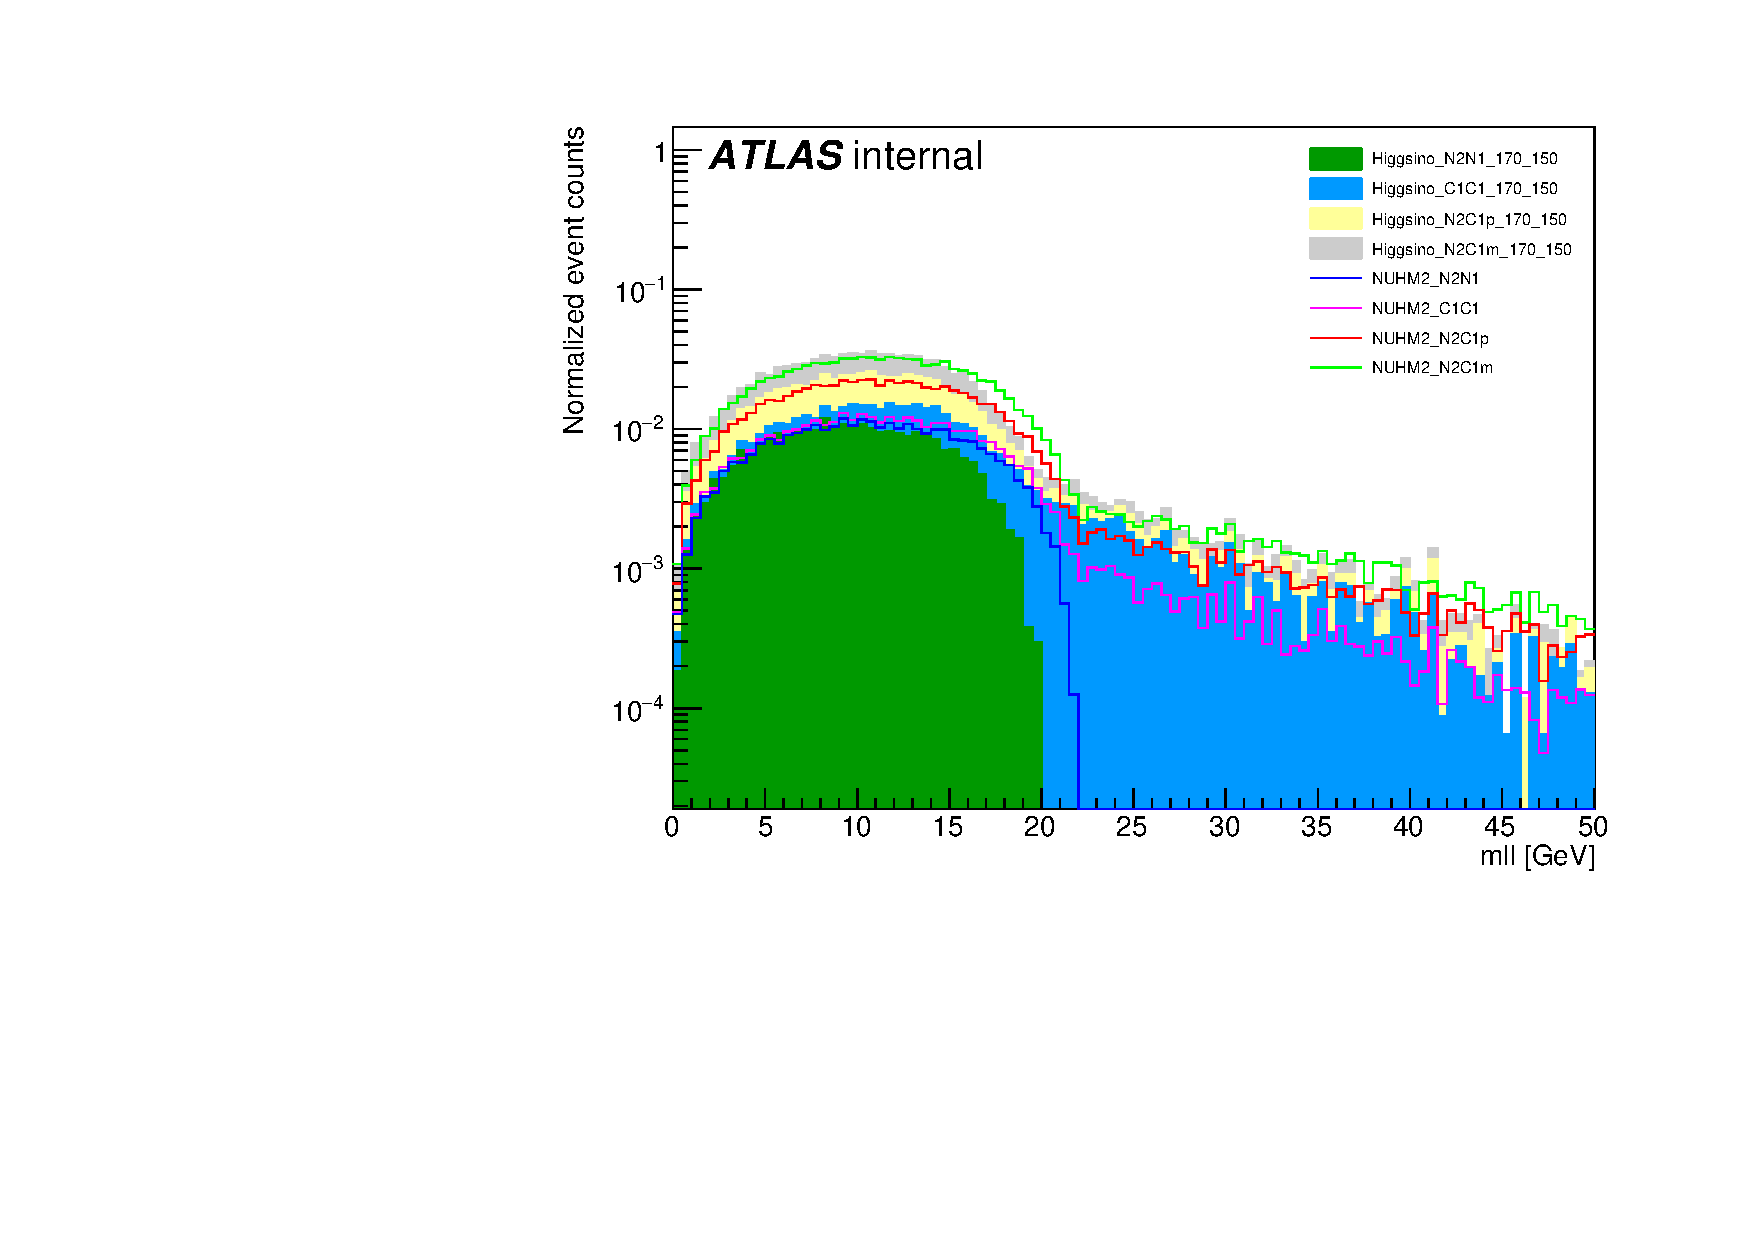
\includegraphics[scale=0.4]{mll.pdf}
%             \caption{$m_{\ell\ell}$}
%         \end{subfigure}
%         \begin{subfigure}[b]{0.48\textwidth}
%             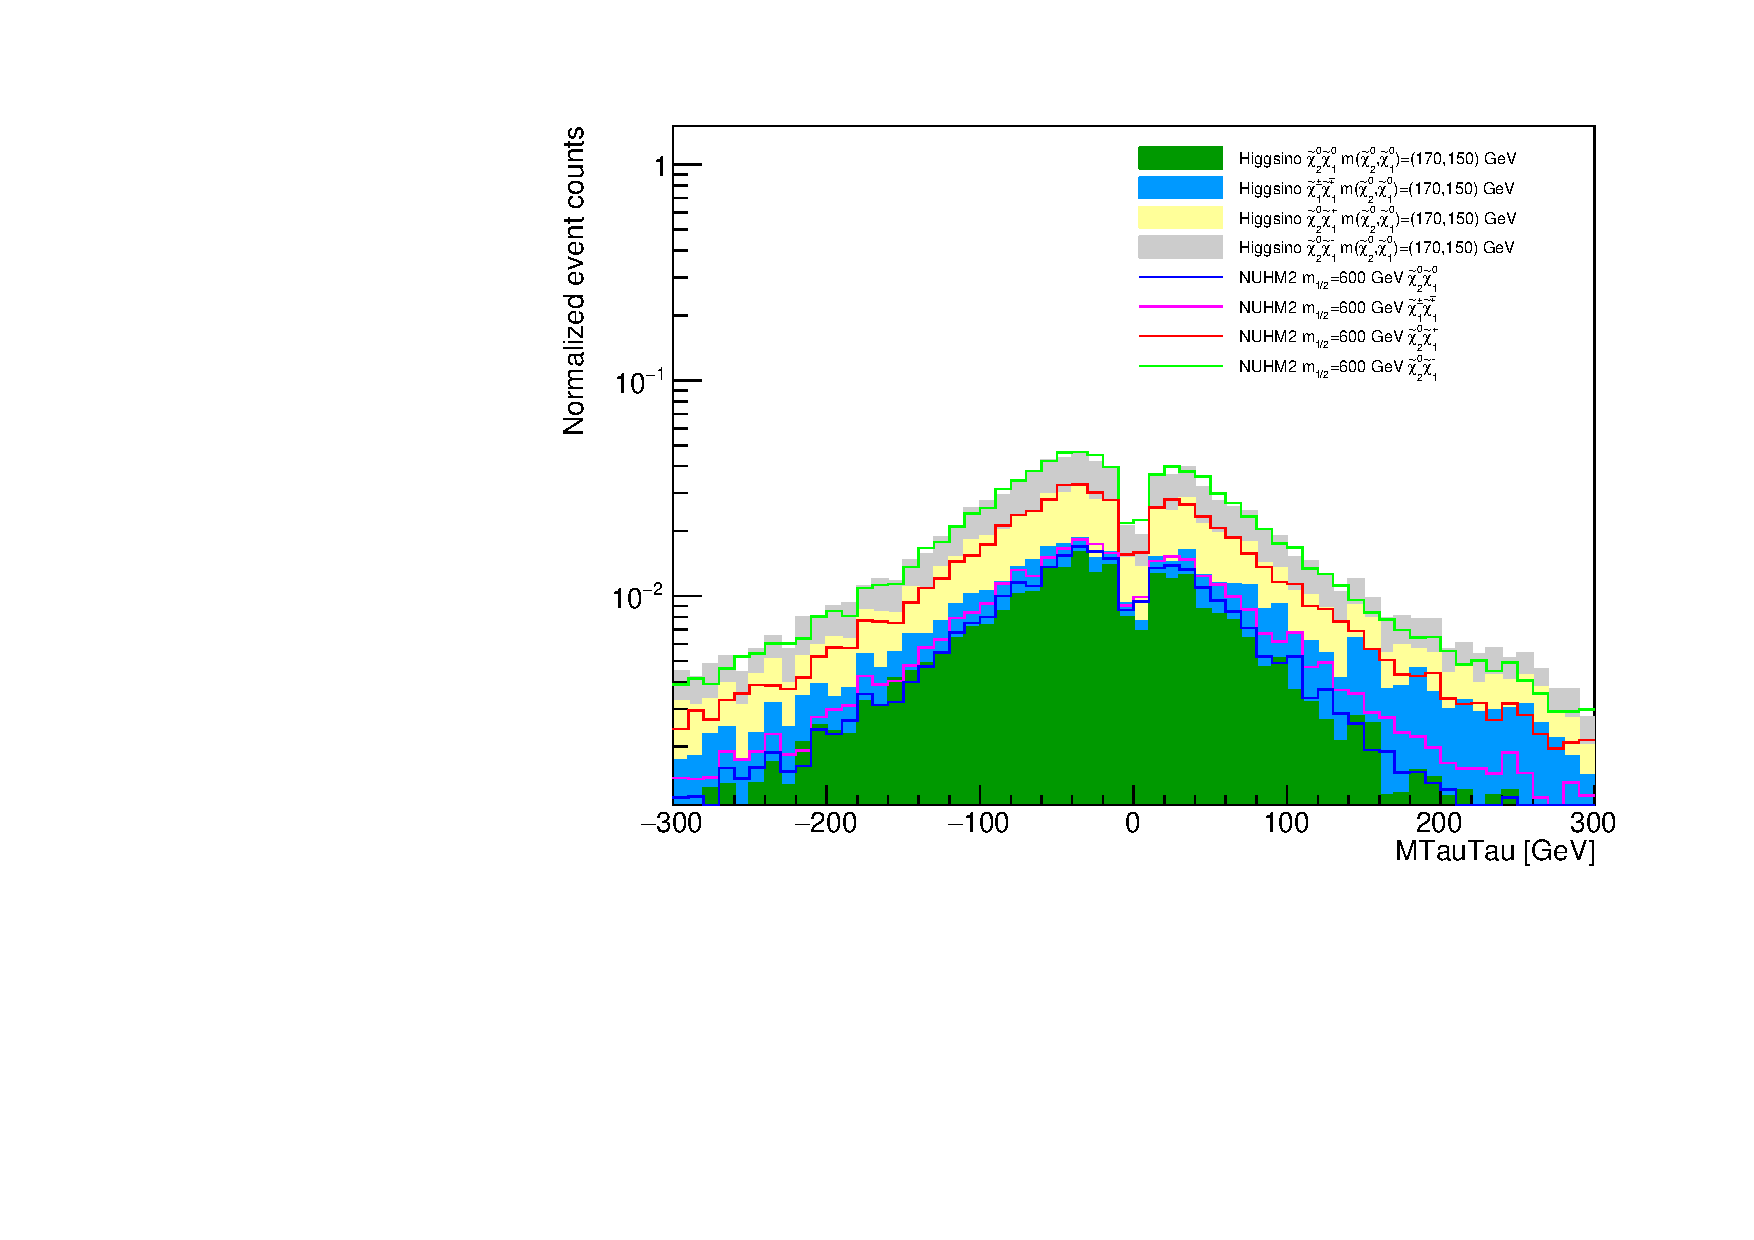
\includegraphics[scale=0.4]{MTauTau.pdf}
%             \caption{$m_{\tau\tau}$}
%         \end{subfigure}
%         \begin{subfigure}[b]{0.48\textwidth}
%             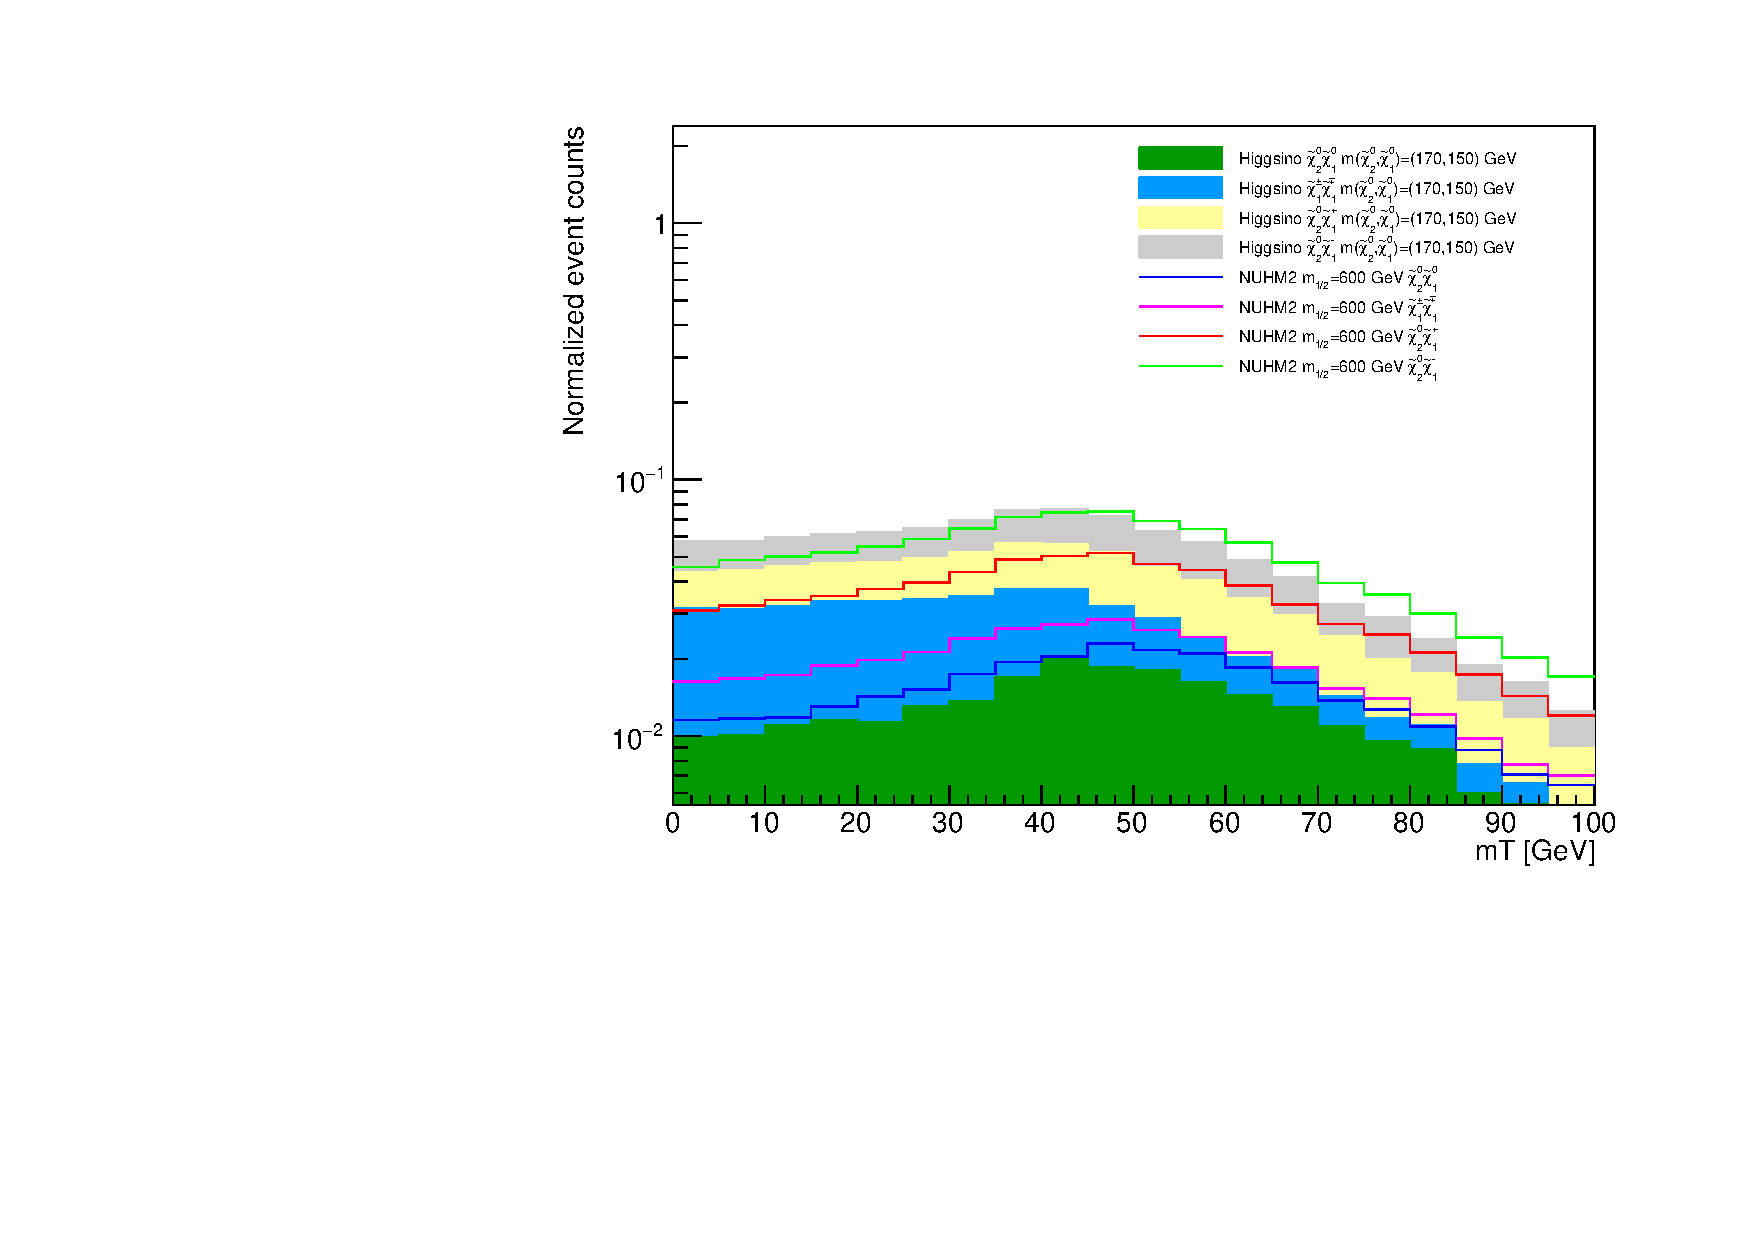
\includegraphics[scale=0.4]{mT.pdf}
%             \caption{$m_{T}$}
%         \end{subfigure}
%         \begin{subfigure}[b]{0.48\textwidth}
%             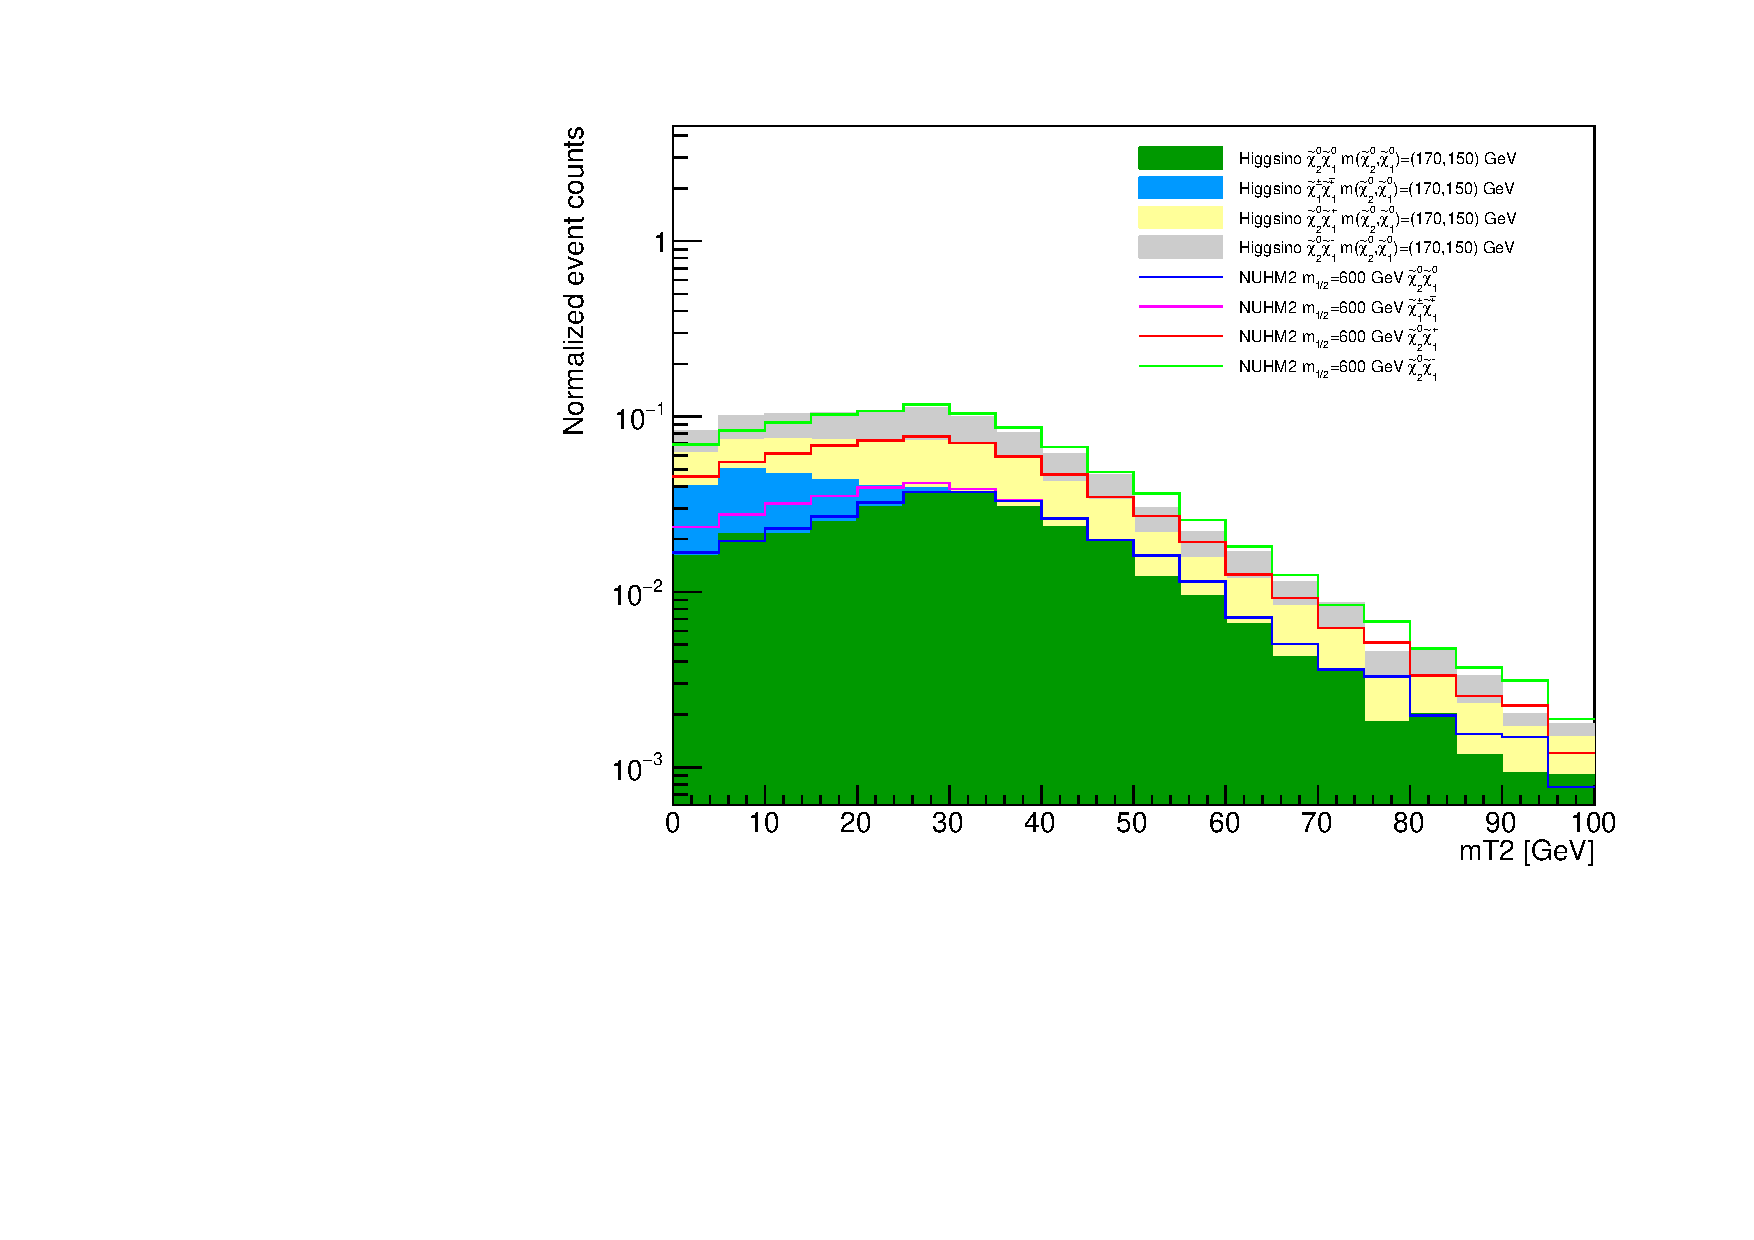
\includegraphics[scale=0.4]{mT2.pdf}
%             \caption{$m_{T2}$}
%         \end{subfigure}
%     \end{center}
%     \caption{The invariant mass $m_{\ell\ell}$ and $m_{\tau\tau}$ distributions and the transverse mass $m_\mathrm{T}$ and $m_\mathrm{T2}$ distributions.
%     The first two leading baseline leptons are used to calculate the $m_{\ell\ell}$ which contains a hump and a tail region.
%     The $\widetilde{\chi}^{0}_{2} \widetilde{\chi}^{0}_{1}$ contributes to the hump only and the tail is contributed by the decay products containing the chargino $\widetilde{\chi}^{\pm}_{1}$.
%     The Eq.~(\ref{eq:event_mtautau}) is used to calculate the di-tau invariant mass $m_{\tau\tau}$.
%     The first or first two leading signal leptons and \met are used to evaluate the transverse mass $m_\mathrm{T}$ and $m_\mathrm{T2}$, respectively.
%     Four different production channels, $\widetilde{\chi}^{0}_{2}\widetilde{\chi}^{0}_{1}$, $\widetilde{\chi}^{0}_{2}\widetilde{\chi}^{+}_{1}$, $\widetilde{\chi}^{0}_{2}\widetilde{\chi}^{-}_{1}$, and $\widetilde{\chi}^{\pm}_{1}\widetilde{\chi}^{\mp}_{1}$, for the NUHM2 and the simplified Higgsino model are considered.
%     The distributions of four productions are combined and normalized to equal area.}
%     \label{fig:results_nuhm2_mll_mtautau_mT_mT2}
% \end{figure}

% \begin{figure}[htbp]
%     \begin{center}
%         \begin{subfigure}[b]{0.48\textwidth}
%             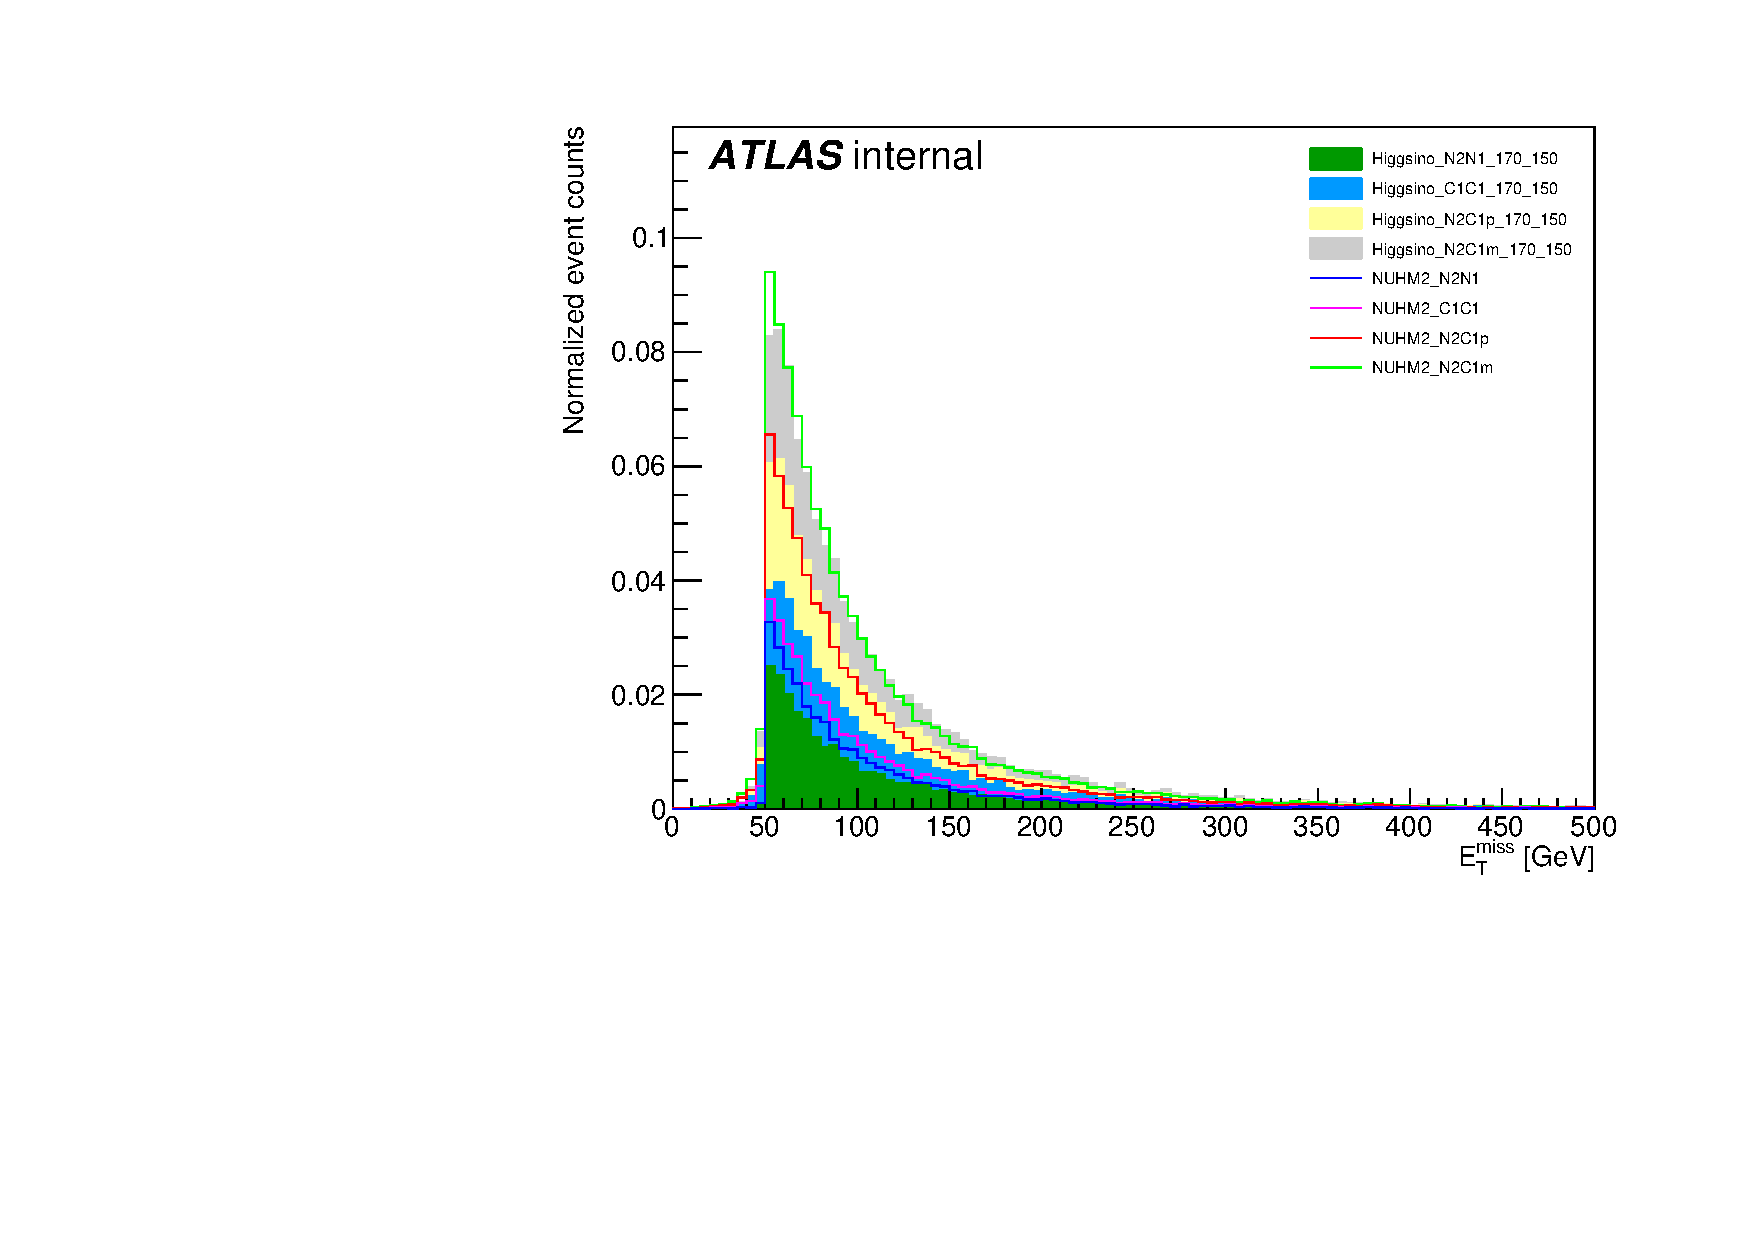
\includegraphics[scale=0.4]{met.pdf}
%             \caption{\met}
%         \end{subfigure}
%         \begin{subfigure}[b]{0.48\textwidth}
%             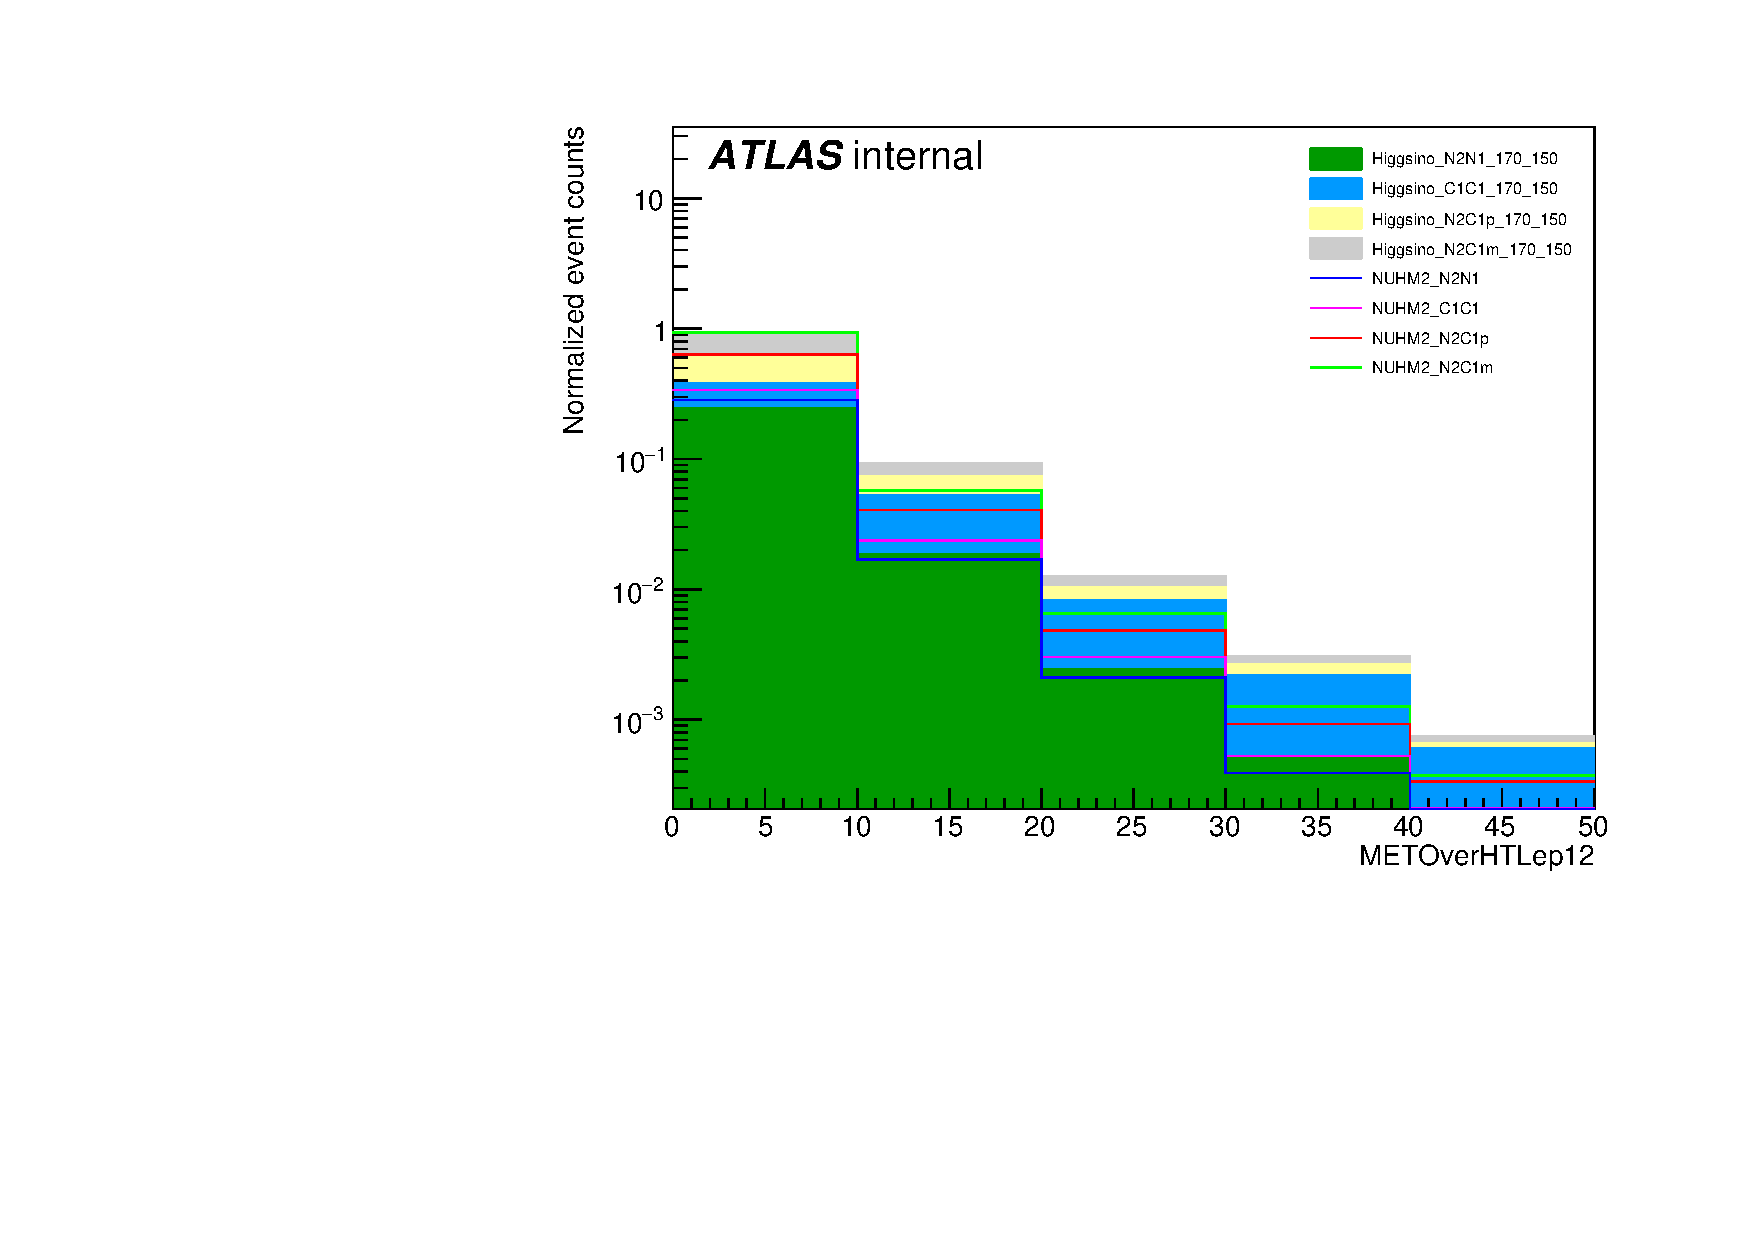
\includegraphics[scale=0.4]{METOverHTLep12.pdf}
%             \caption{$\met/H_\mathrm{T}^\mathrm{lepton}$}
%         \end{subfigure}
%         \begin{subfigure}[b]{0.48\textwidth}
%             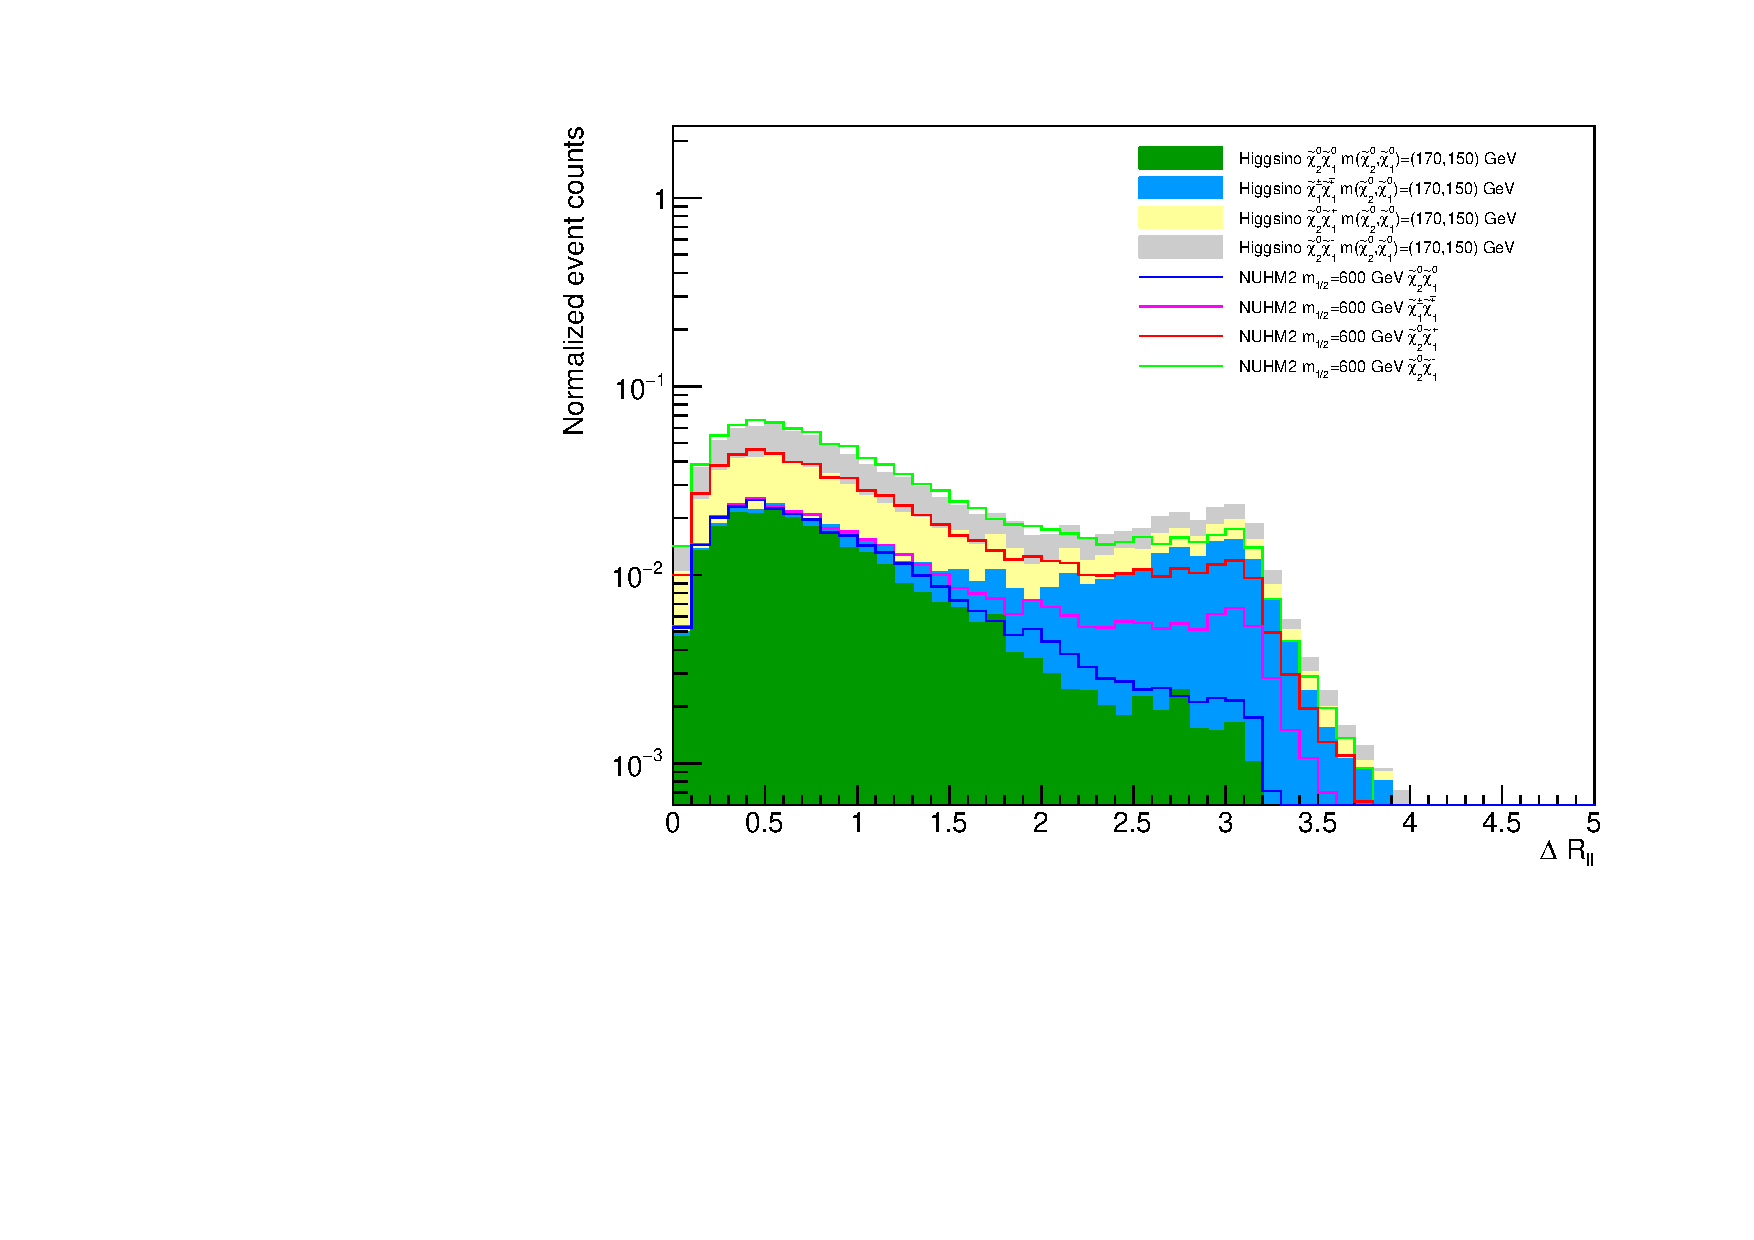
\includegraphics[scale=0.4]{Rll.pdf}
%             \caption{$\Delta R(\ell_{1}, \ell_{2})$}
%         \end{subfigure}
%         \begin{subfigure}[b]{0.48\textwidth}
%             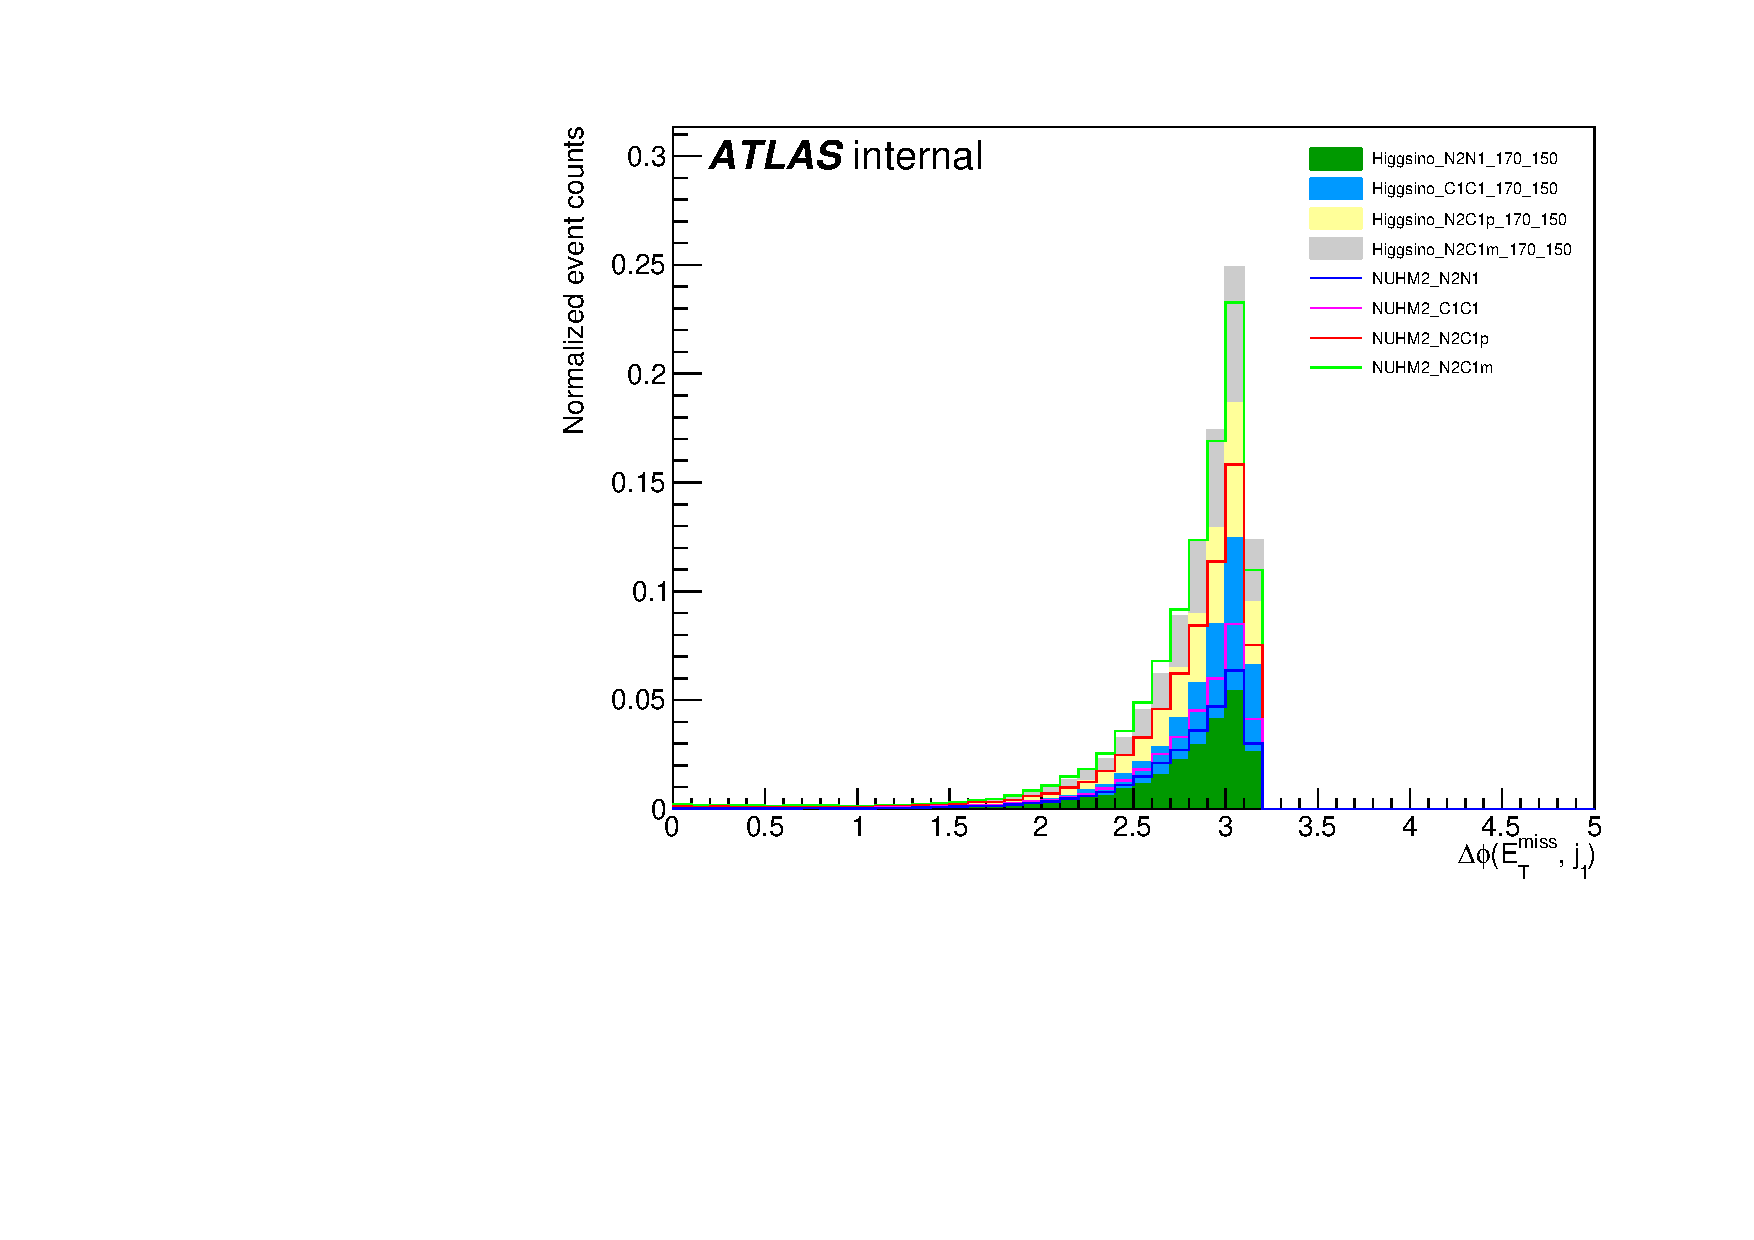
\includegraphics[scale=0.4]{dphiMin1.pdf}
%             \caption{$\Delta \phi(\met, j_{1})$}
%         \end{subfigure}
%     \end{center}
%     \caption{The \met, $\met/H_\mathrm{T}^\mathrm{lepton}$, $\Delta R(\ell_{1}, \ell_{2})$, and $\Delta \phi(\met, j_{1})$ distributions.
%     The $H_\mathrm{T}^\mathrm{lepton}$ is the scalar sum of the first two leading baseline leptons \pt only.
%     The distance $\Delta R(\ell_{1}, \ell_{2})$ is calculated by the first two leading baseline leptons and the $\Delta \phi(\met, j_{1})$ uses \met and first leading signal jet.
%     Four different production channels, $\widetilde{\chi}^{0}_{2}\widetilde{\chi}^{0}_{1}$, $\widetilde{\chi}^{0}_{2}\widetilde{\chi}^{+}_{1}$, $\widetilde{\chi}^{0}_{2}\widetilde{\chi}^{-}_{1}$, and $\widetilde{\chi}^{\pm}_{1}\widetilde{\chi}^{\mp}_{1}$, for the NUHM2 and the simplified Higgsino model are considered.
%     The distributions of four productions are combined and normalized to equal area.}
%     \label{fig:results_nuhm2_met_METOverHTLep12_Rll_dphiMin1}
% \end{figure}

%%%
%%%
%%%

\section{NUHM2 interpretation using the $m_{\ell \ell}$ reweighting method}
\label{sec:results_mll_reweighting}
The mass eigenstates of the electroweakinos are composed of different mixtures of Bino, Wino, and Higgsino in the compressed scenario.
The simplified Higgsino model signal samples are generated using a mixture of Higgsinos and the cross-sections are calculated accordingly.
Since the main difference between NUHM2 and the simplified Higgsino model is the invariant mass distribution of the two leptons due to the mass splittings of $\Delta m(\widetilde{\chi}^{0}_{2}, \widetilde{\chi}^{0}_{1})$ and $\Delta m(\widetilde{\chi}^{\pm}_{1}, \widetilde{\chi}^{0}_{1})$, the simplified Higgsino model signal samples could be used for the NUHM2 interpretation by scaling the $m_{\ell \ell}$ distribution and cross-sections.

The invariant mass distribution can be calculated by
%
\begin{align}
    \frac{d\Gamma}{2mdm}
    & \propto \frac{\sqrt{m^{4}-m^{2}(m^{2}_{\widetilde{\chi}^{0}_{2}} + m^{2}_{\widetilde{\chi}^{0}_{1}})+(m^{2}_{\widetilde{\chi}^{0}_{2}} - m^{2}_{\widetilde{\chi}^{0}_{1}})^{2}}}{(m^{2} - m^{2}_{Z})^{2}}\\
    & \times \Big[-2m^{4}+m^{2}(m^{2}_{\widetilde{\chi}^{0}_{1}} \pm 6 m_{\widetilde{\chi}^{0}_{1}} m_{\widetilde{\chi}^{0}_{1}} + m^{2}_{\widetilde{\chi}^{0}_{2}})+(m^{2}_{\widetilde{\chi}^{0}_{1}} - m^{2}_{\widetilde{\chi}^{0}_{2}})^{2}\Big]
    \label{eq:results_mll_formula}
\end{align}
%
where the $\pm$ depends on the assumption of the mixture of the eigenstates.
The ``$+$'' is for the NUHM2 and ``$-$'' is for the simplified Higgsino model.
The detail of the reweighted $m_{\ell \ell}$ distributions are shown in Sect.~\ref{subsec:results_reweighted_mll_distributions}, the validations of the $m_{\ell \ell}$ reweighting method are shown in Sect.~\ref{subsec:results_reweighted_validations}, and the results are shown in Sect.~\ref{subsec:results_mll_reweighting_interpretation}.

%%%
%%%
%%%

\subsection{The reweighted $m_{\ell \ell}$ distributions}
\label{subsec:results_reweighted_mll_distributions}
Using the $m_{\ell \ell}$ reweighting method, the simplified Higgsino samples can reproduce the NUHM2 distributions at the reconstruction level.
The $m_{\ell \ell}$ distributions for the NUHM2 and the simplified Higgsino samples can be calculated by the $m_{\widetilde{\chi}^{0}_{1}}$ and $m_{\widetilde{\chi}^{0}_{1}}$ using Eq.~\ref{eq:results_mll_formula}.
From the ratio of the $m_{\ell \ell}$ distributions between two models and the cross-section weight, the event weighting is performed.
The event-by-event reweighting of the $m_{\ell \ell}$ distributions between two models is examined at the truth level.

A number of details have to be considered in the $m_{\ell \ell}$ reweighting procedure.
The reweighting method only considers the $\widetilde{\chi}^{0}_{2} \widetilde{\chi}^{0}_{1}$ and $\widetilde{\chi}^{0}_{2} \widetilde{\chi}^{\pm}_{1}$ productions because the $\widetilde{\chi}^{\pm}_{1} \widetilde{\chi}^{\mp}_{1}$ contributes mainly to the tail region of the $m_{\ell \ell}$ distribution which is not sensitive in this analysis.
% The $\Delta m = m_{\widetilde{\chi}^{2}_{1}} - m_{\widetilde{\chi}^{0}_{1}}$ of the simplified Higgsino sample has to be higher than and compared to the one in the NUHM2.
% The Higgsino grid points used in the $m_{\ell \ell}$ reweighting method have to be as close as possible to the  $m_{\widetilde{\chi}^{0}_{2}}$ and $m_{\widetilde{\chi}^{0}_{1}}$ in NUHM2.
The grid points have to be selected with similar $m_{\widetilde{\chi}^{0}_{2}}$, $m_{\widetilde{\chi}^{0}_{1}}$, and $\Delta m = m_{\widetilde{\chi}^{2}_{1}} - m_{\widetilde{\chi}^{0}_{1}}$.
Table~\ref{tab:results_reweighting_grid_points} shows the grid points used for the $m_{\ell \ell}$ reweighting.
%
\begin{table}[htp]
    \begin{center}
        {\footnotesize
            \begin{tabular}{llllllll}
                \hline
                \hline
                \multirow{2}{*}{$m_{1/2}$~[{\GeV}]} & \multicolumn{3}{c}{NUHM2} & \multicolumn{3}{c}{Simplified Higgsino} & \multirow{2}{*}{$\delta$}\\
                & $m_{\widetilde{\chi}^{0}_{2}}$ & $m_{\widetilde{\chi}^{0}_{1}}$ & $\Delta m$ & $m_{\widetilde{\chi}^{0}_{2}}$ & $m_{\widetilde{\chi}^{0}_{1}}$ & $\Delta m$ & \\
                \hline
                350 & 161.68 & 115.62 & 46.06 & 160 & 100 & 60 & 13.94\\
                400 & 161.14 & 122.97 & 38.17 & 190 & 150 & 40 & 1.8\\
                500 & 160.30 & 132.28 & 28.02 & 190 & 150 & 40 & 11.98\\
                600 & 159.66 & 137.61 & 22.05 & 190 & 150 & 40 & 17.95\\
                700 & 159.17 & 140.98 & 18.19 & 170 & 150 & 20 & 1.81\\
                800 & 158.78 & 143.29 & 15.49 & 170 & 150 & 20 & 4.51\\
                \hline
                \hline
            \end{tabular}
        }
    \end{center}
    \caption{The grid points of NUHM2 and simplified Higgsino samples used for the $m_{\ell \ell}$ reweighting.
    The smaller $\delta = \Delta m_{Higgsino} - \Delta m_{NUHM2}$ the better reweighting results.}
    \label{tab:results_reweighting_grid_points}
\end{table}%
%
Table~\ref{tab:results_reweighting_cross_section_ratio} shows the cross-section weights used for the $m_{\ell \ell}$ reweighting.

\begin{table}[htp]
    \begin{center}
        {\footnotesize
            \begin{tabular}{cllll}
                \hline
                \hline
                $m_{1/2}$~[{\GeV}] & $\widetilde{\chi}^{0}_{2} \widetilde{\chi}^{0}_{1}$ & $\widetilde{\chi}^{\pm}_{1} \widetilde{\chi}^{\mp}_{1}$ & $\widetilde{\chi}^{0}_{2} \widetilde{\chi}^{+}_{1}$ & $\widetilde{\chi}^{0}_{2} \widetilde{\chi}^{-}_{1}$\\
                \hline
                350 & 0.5004 & 0.8093 & 0.7533 & 0.7517\\
                400 & 1.4061 & 1.8576 & 1.6181 & 1.6892\\
                500 & 1.4842 & 1.6071 & 1.6120 & 1.6803\\
                600 & 1.4962 & 1.4889 & 1.6054 & 1.6694\\
                700 & 1.1811 & 1.1428 & 1.1703 & 1.1918\\
                800 & 1.1731 & 1.1076 & 1.1673 & 1.1896\\
                \hline
                \hline
            \end{tabular}
        }
    \end{center}
    \caption{The cross-section weight used for the $m_{\ell \ell}$ reweighting.
    The weights are obtained by calculating the ratio between $\sigma$(NUHM2) and $\sigma$(Higgsino).}
    \label{tab:results_reweighting_cross_section_ratio}
\end{table}%
% \begin{table}[htp]
%     \begin{center}
%         {\footnotesize
%             \begin{tabular}{cllll}
%                 \hline
%                 \hline
%                 $m_{1/2}$~[{\GeV}] & $\widetilde{\chi}^{0}_{2} \widetilde{\chi}^{0}_{1}$ & $\widetilde{\chi}^{\pm}_{1} \widetilde{\chi}^{\mp}_{1}$ & $\widetilde{\chi}^{0}_{2} \widetilde{\chi}^{+}_{1}$ & $\widetilde{\chi}^{0}_{2} \widetilde{\chi}^{-}_{1}$\\
%                 \hline
%                 350 & 0.50048910367 & 0.80929519789 & 0.75334324027 & 0.75165191712\\
%                 400 & 1.40609496035 & 1.85763670956 & 1.61810558673 & 1.68915991429\\
%                 500 & 1.48420174312 & 1.60709633189 & 1.61195100629 & 1.68026588159\\
%                 600 & 1.49620688527 & 1.48886200733 & 1.60540039476 & 1.66943310114\\
%                 700 & 1.18114972806 & 1.14281934535 & 1.17032101263 & 1.19178384310\\
%                 800 & 1.17312186754 & 1.10758453419 & 1.16731420042 & 1.18958896195\\
%                 \hline
%                 \hline
%             \end{tabular}
%         }
%     \end{center}
%     \caption{The cross-section weight used for the $m_{\ell \ell}$ reweighting.
%     The weights are obtained by calculating the ratio between $\sigma$(NUHM2) and $\sigma$(Higgsino).}
%     \label{tab:results_reweighting_cross_section_ratio}
% \end{table}%

Figure~\ref{fig:results_nuhm2_reweighting} shows the $m_{\ell \ell}$ distributions before and after reweighting for NUHM2 and the simplified Higgsino model.
The blue and green solid lines are the TRUTH $m_{\ell \ell}$ distributions for NUHM2 and simplified Higgsino models, respectively.
The blue and green dashed lines are the theoretical distribution predicted by Eq.~\ref{eq:results_mll_formula}.
Good agreement can be seen between the TRUTH (solid line) and the predicted (dashed line) distributions.
The distribution of the reweighted Higgsino sample is shown in red line which matches well with the NUHM2 (blue solid line).

\begin{figure}[htbp]
    \begin{center}
        \begin{subfigure}[b]{0.48\textwidth}
            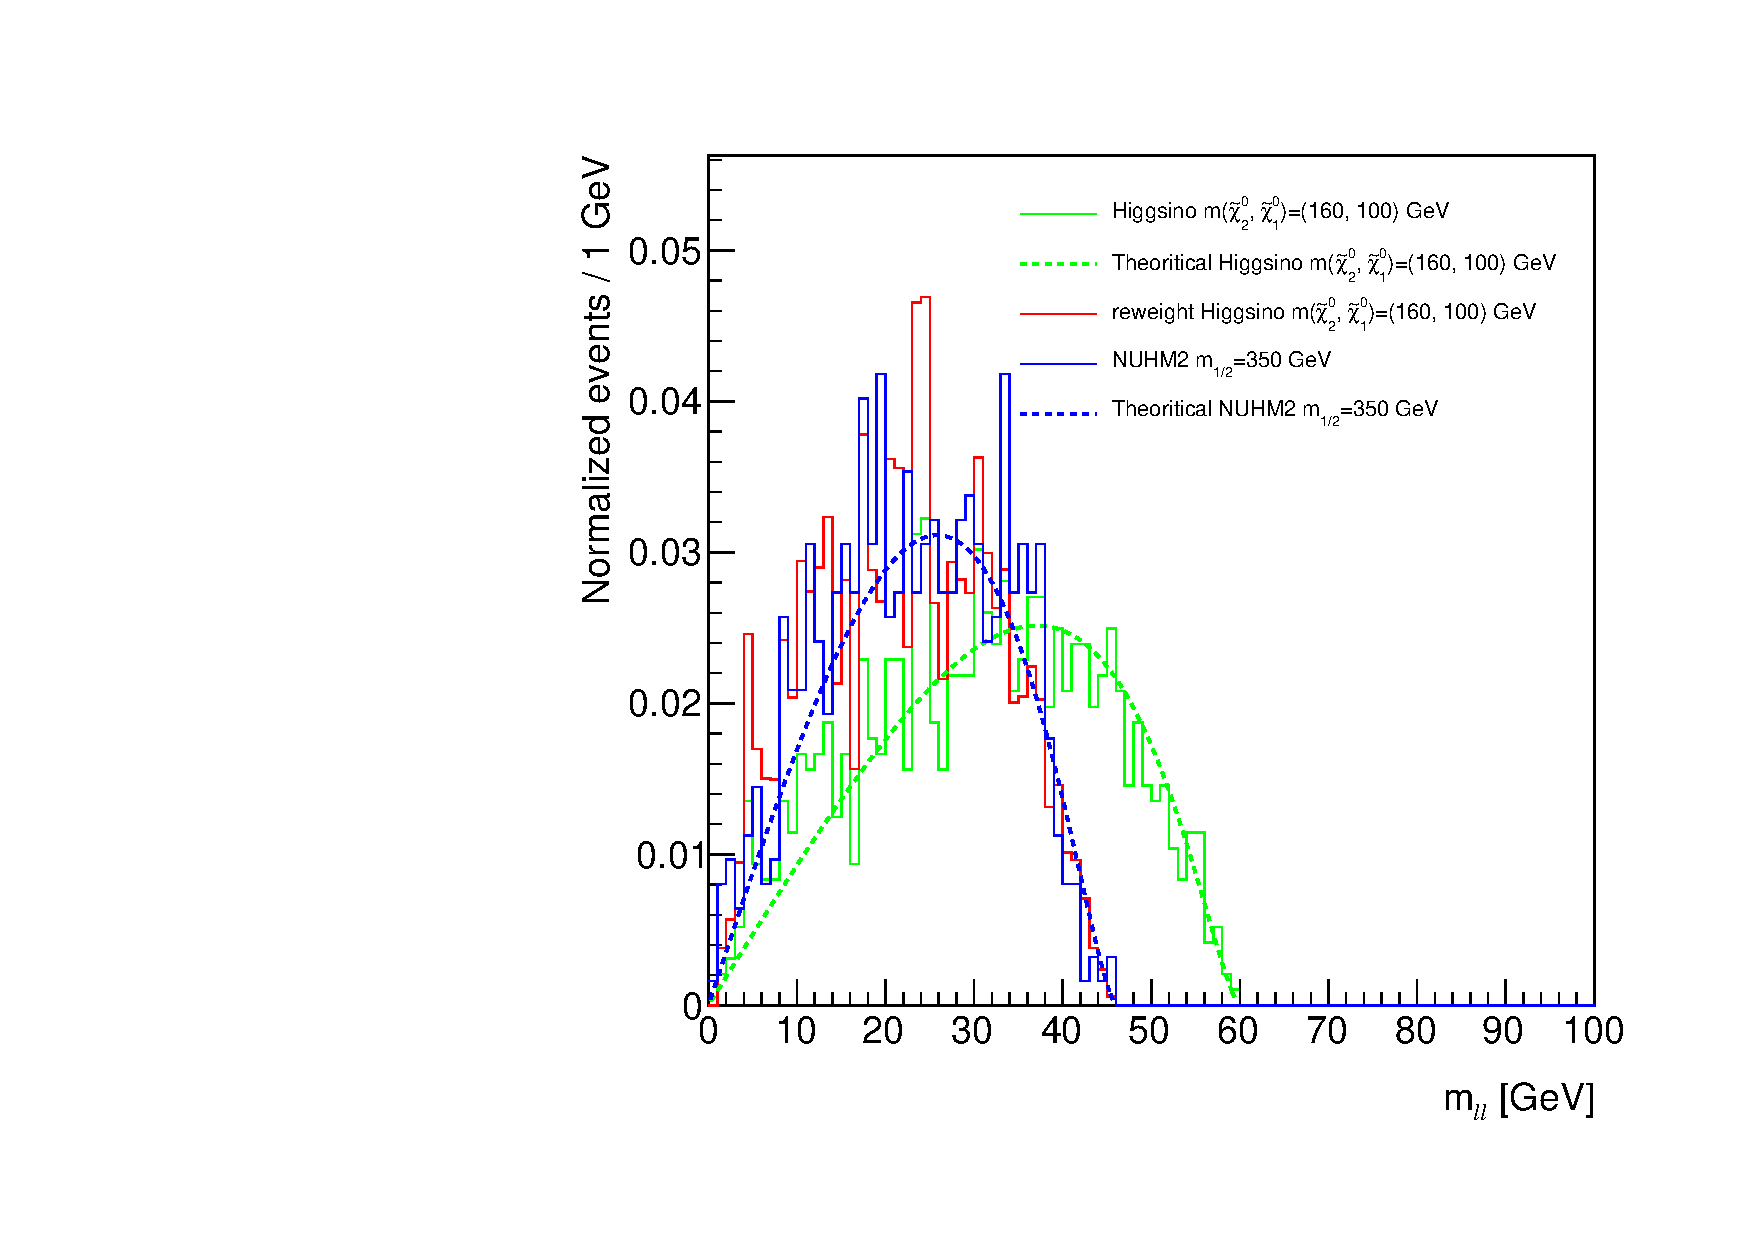
\includegraphics[scale=0.25]{reweight_Lorenzo_Higgsino_160_100_m12_350.pdf}
            \caption{NUHM2 $m_{1/2}=350$~{\GeV}}
        \end{subfigure}
        \begin{subfigure}[b]{0.48\textwidth}
            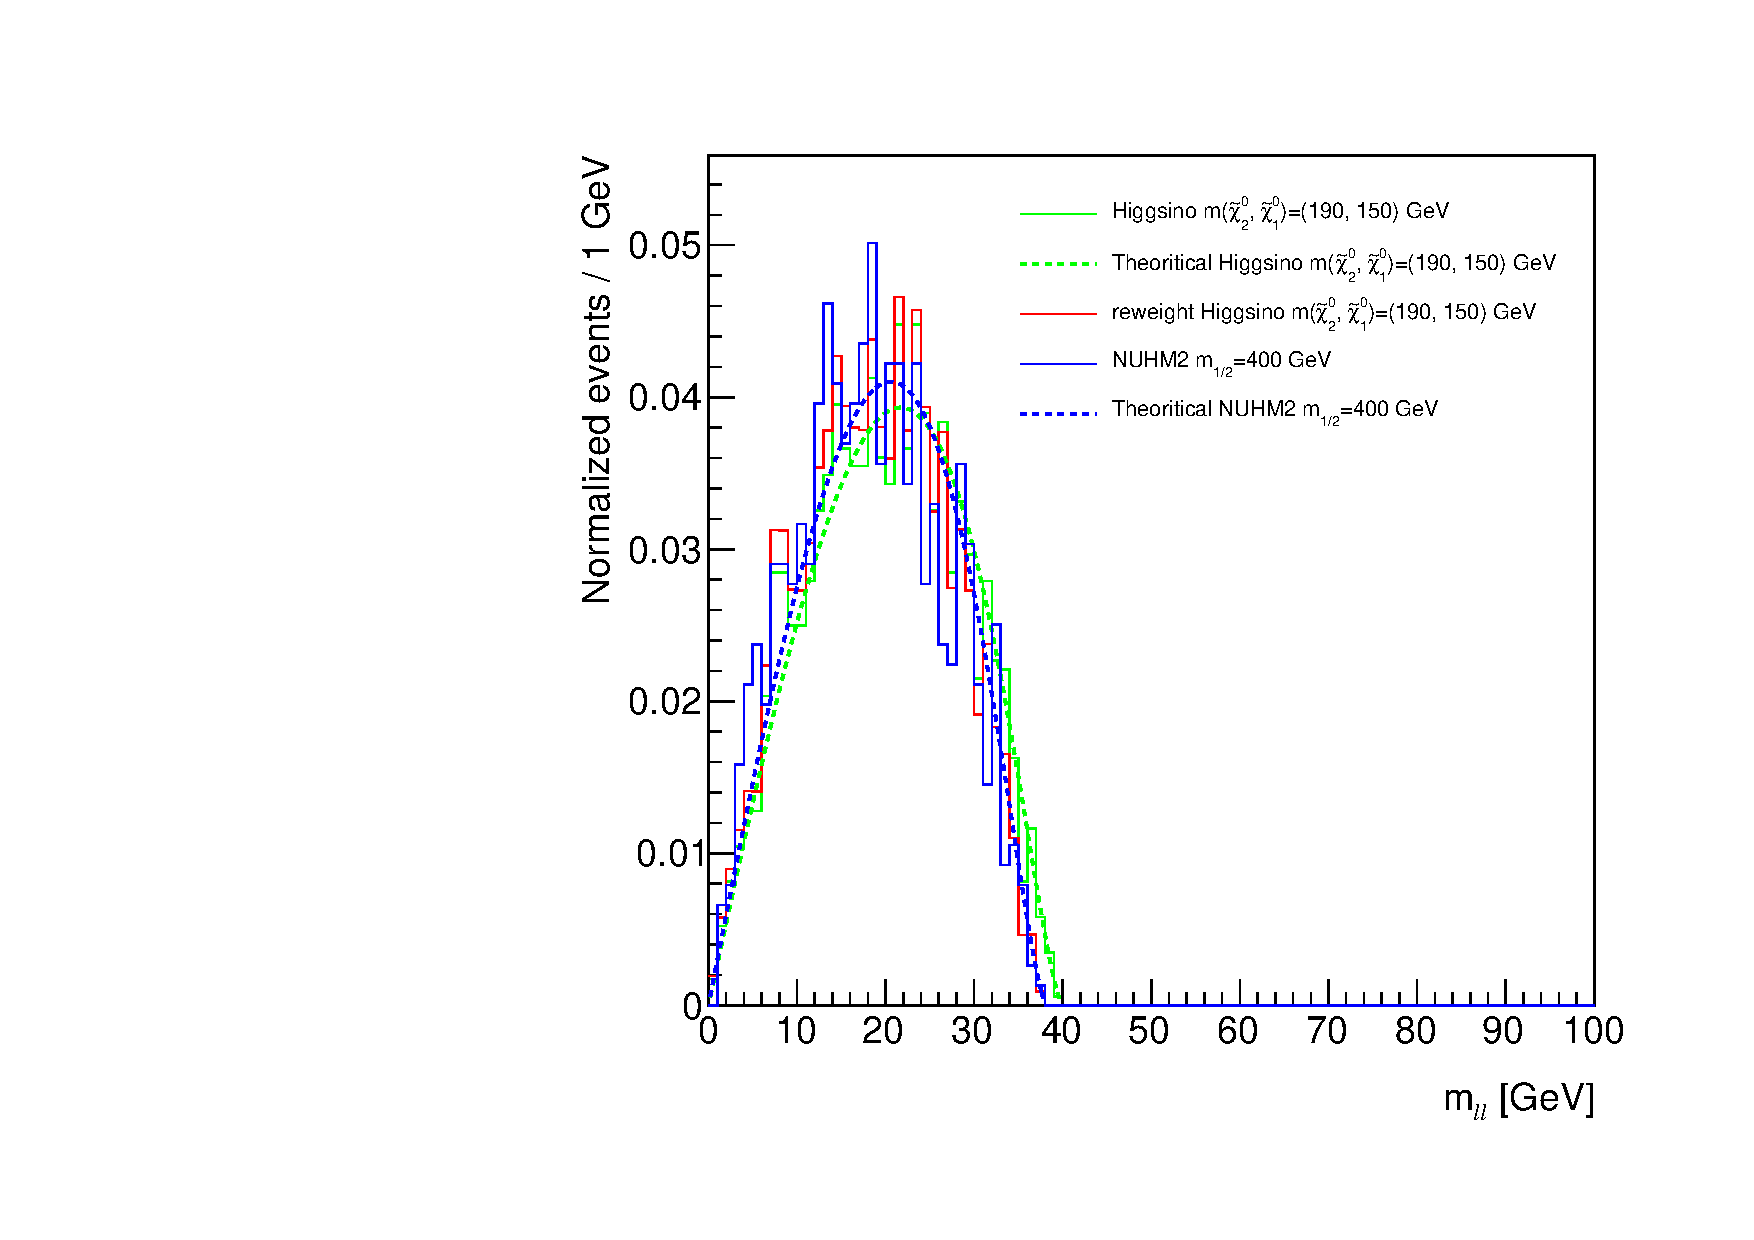
\includegraphics[scale=0.25]{reweight_Lorenzo_Higgsino_190_150_m12_400.pdf}
            \caption{NUHM2 $m_{1/2}=400$~{\GeV}}
        \end{subfigure}
        \begin{subfigure}[b]{0.48\textwidth}
            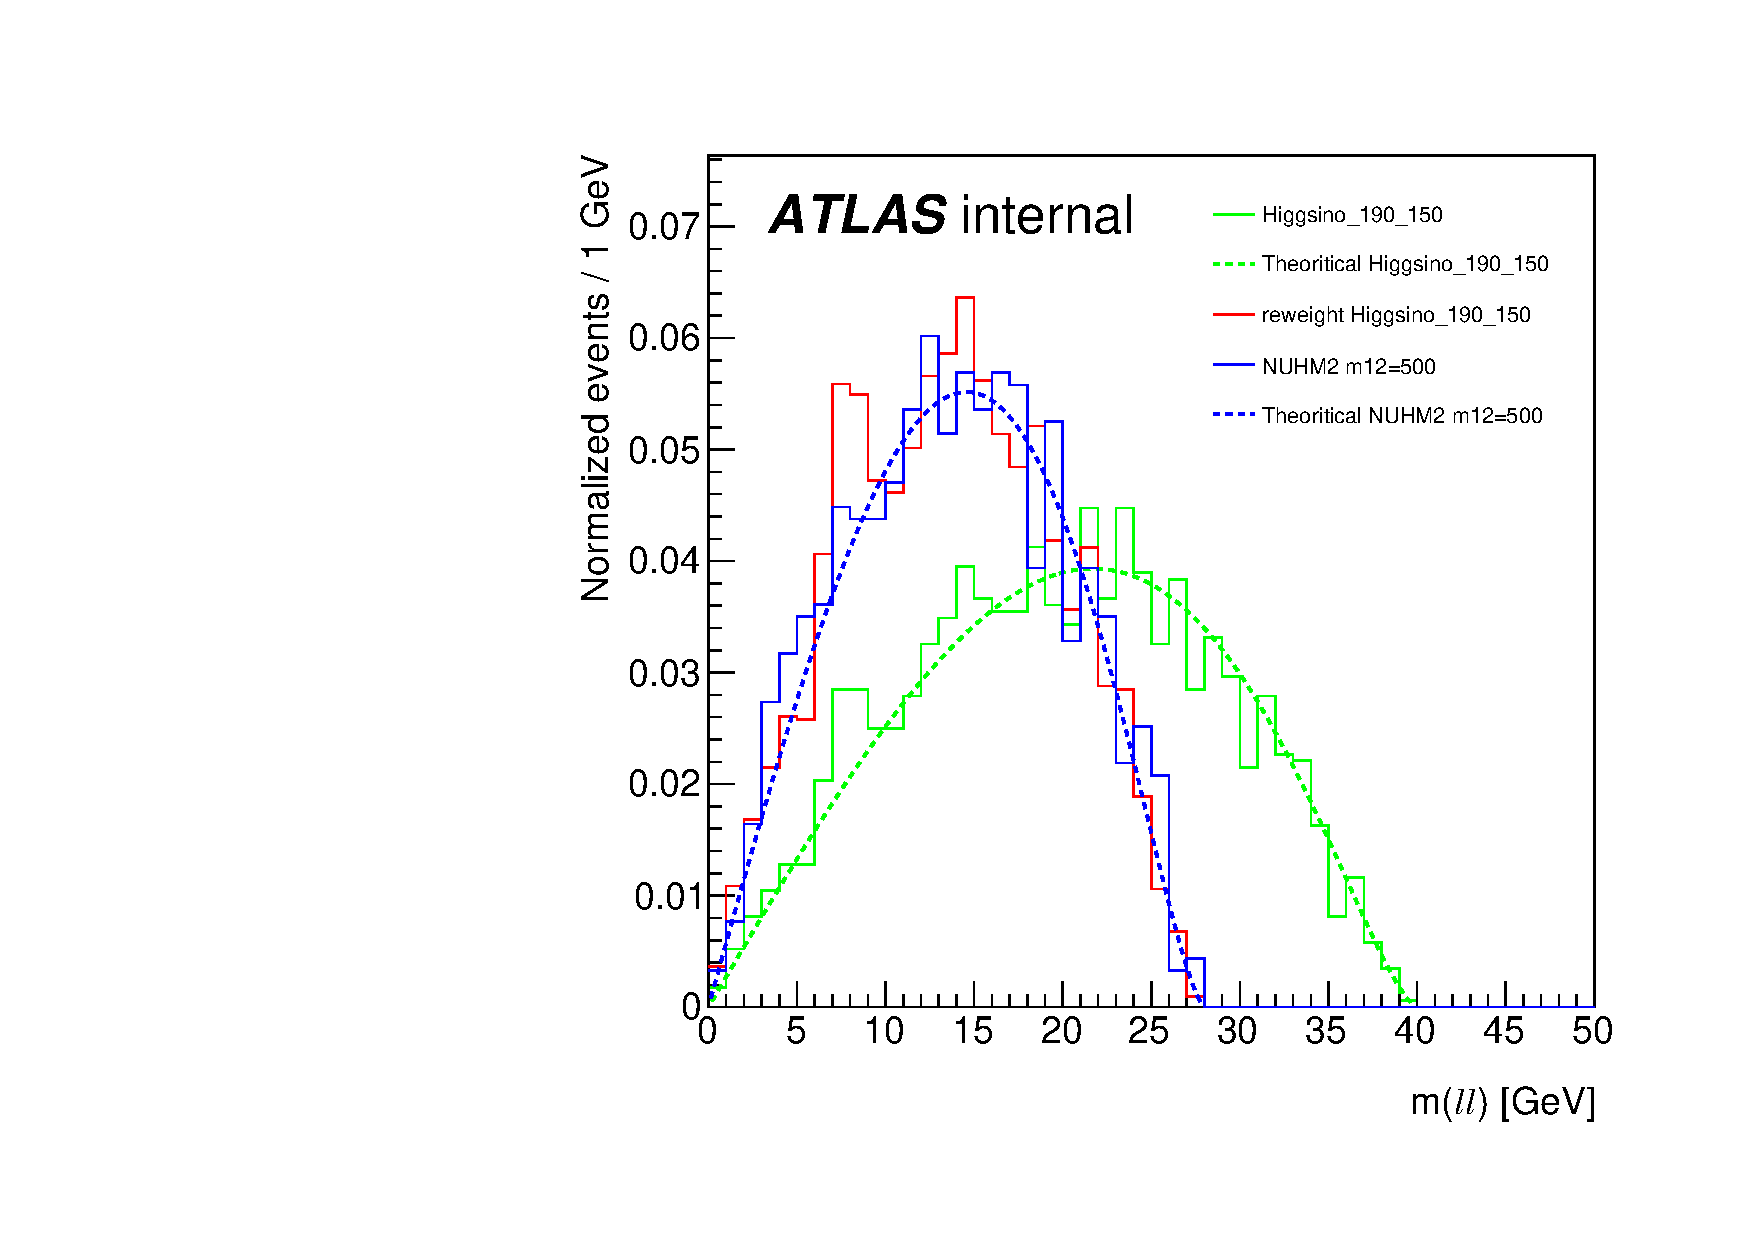
\includegraphics[scale=0.25]{reweight_Lorenzo_Higgsino_190_150_m12_500.pdf}
            \caption{NUHM2 $m_{1/2}=500$~{\GeV}}
        \end{subfigure}
        \begin{subfigure}[b]{0.48\textwidth}
            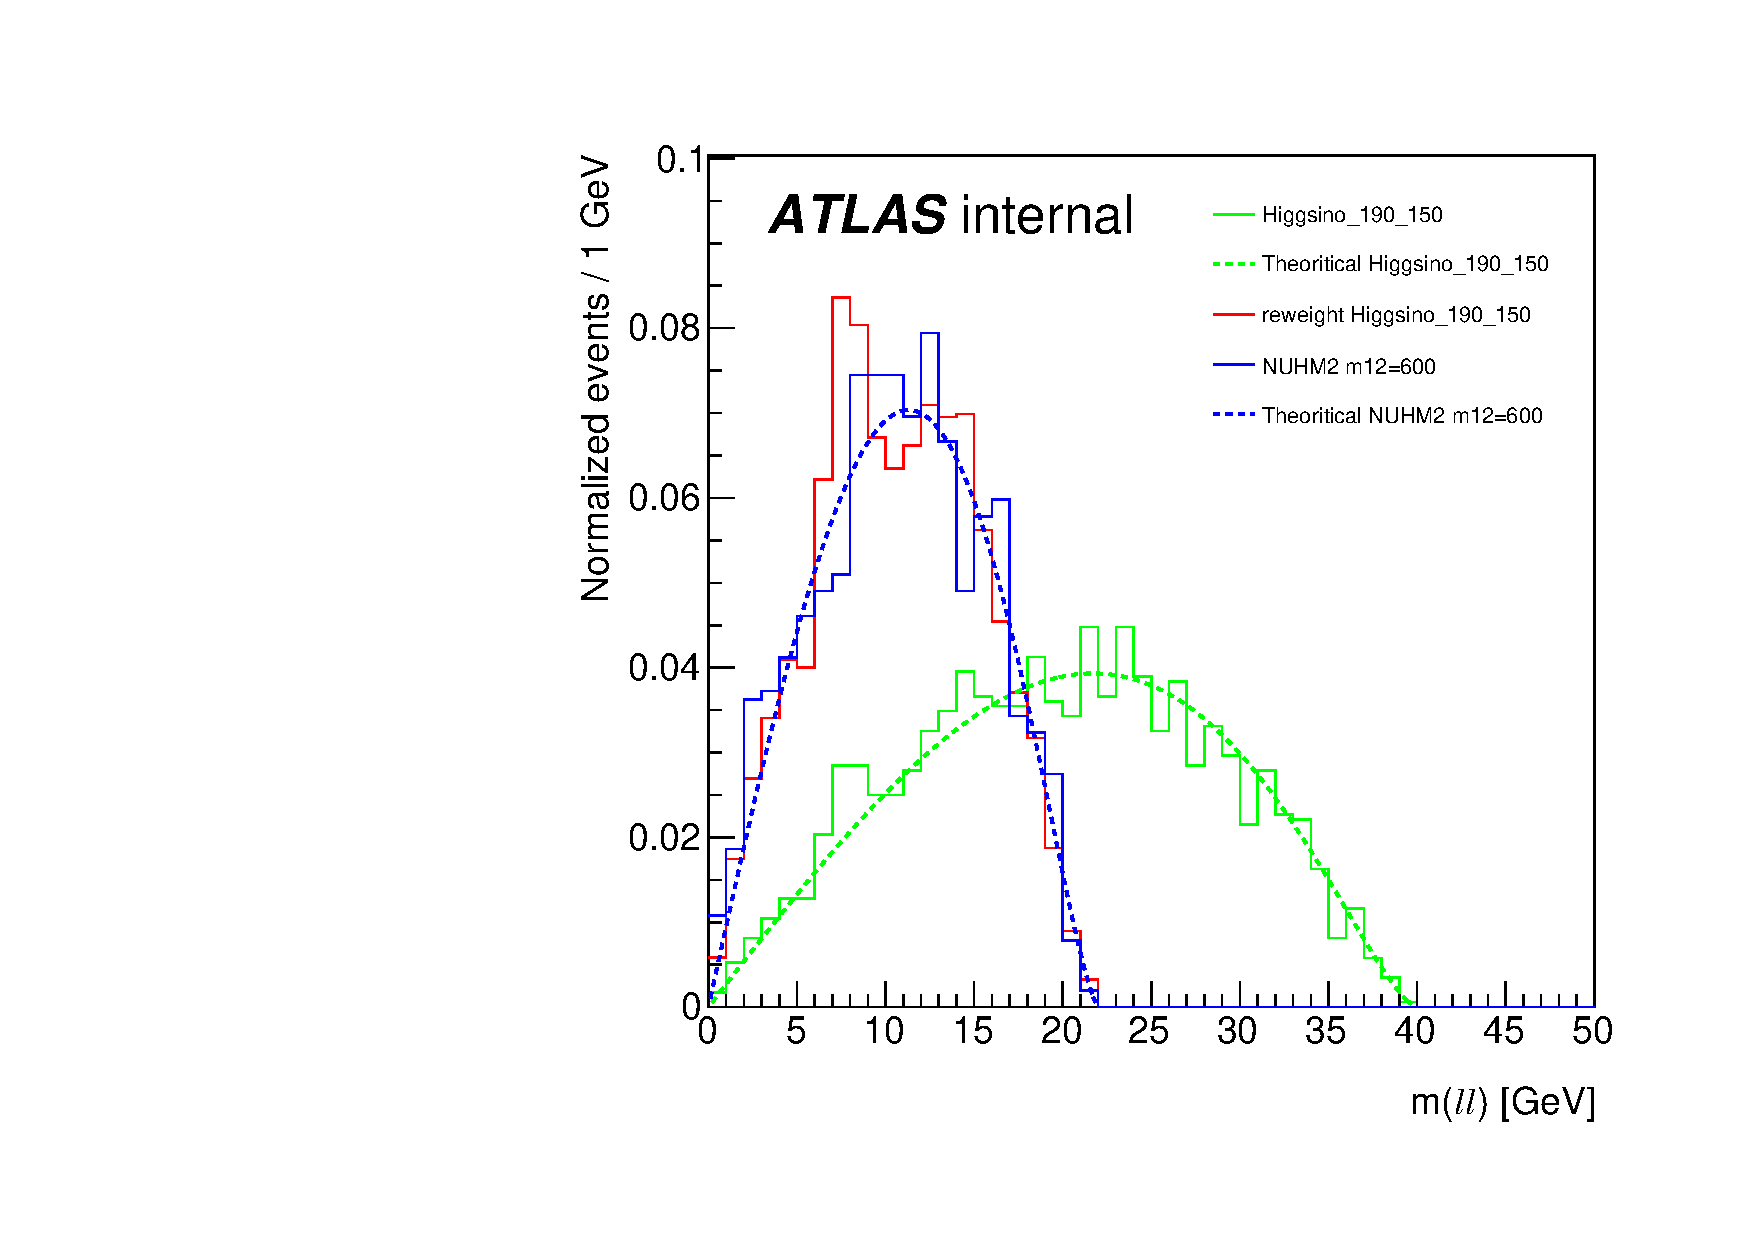
\includegraphics[scale=0.25]{reweight_Lorenzo_Higgsino_190_150_m12_600.pdf}
            \caption{NUHM2 $m_{1/2}=600$~{\GeV}}
        \end{subfigure}
        \begin{subfigure}[b]{0.48\textwidth}
            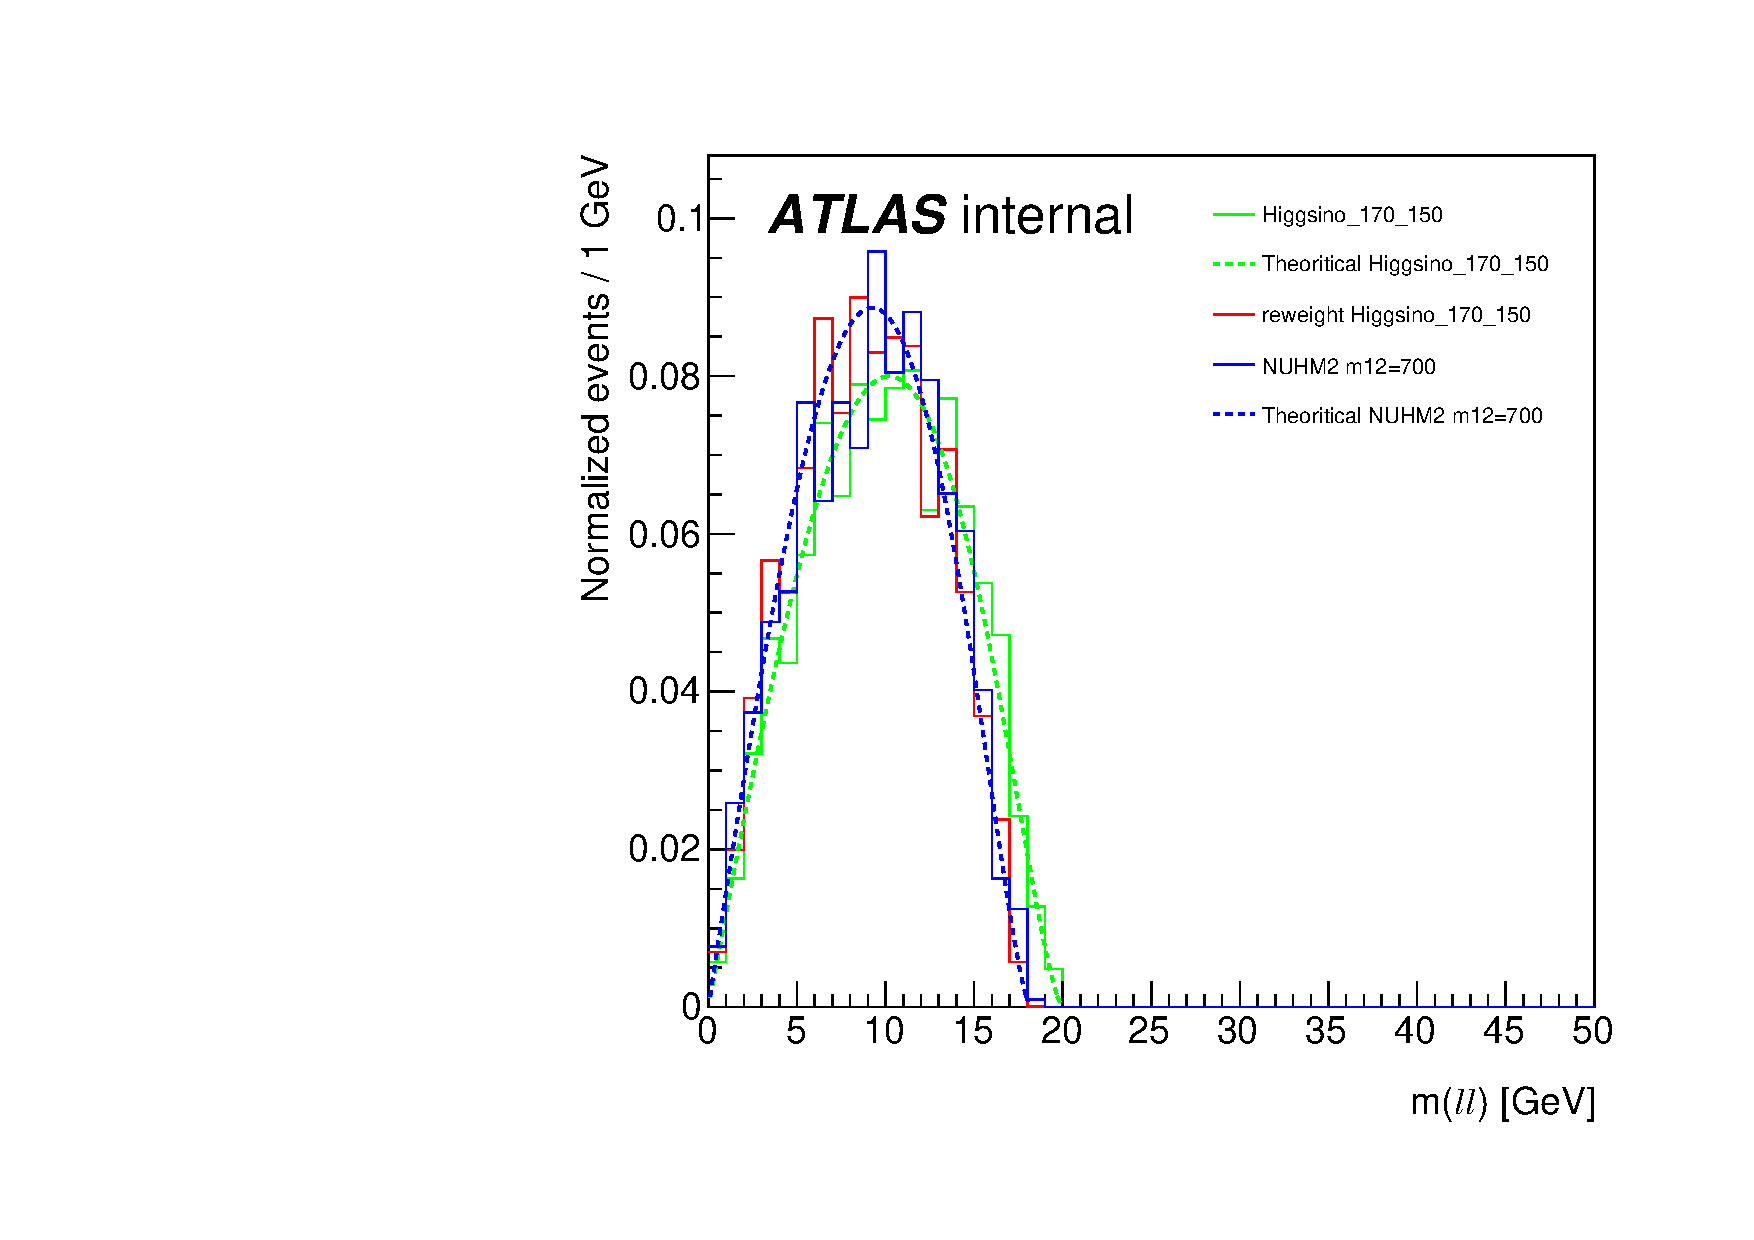
\includegraphics[scale=0.25]{reweight_Lorenzo_Higgsino_170_150_m12_700.pdf}
            \caption{NUHM2 $m_{1/2}=700$~{\GeV}}
        \end{subfigure}
        \begin{subfigure}[b]{0.48\textwidth}
            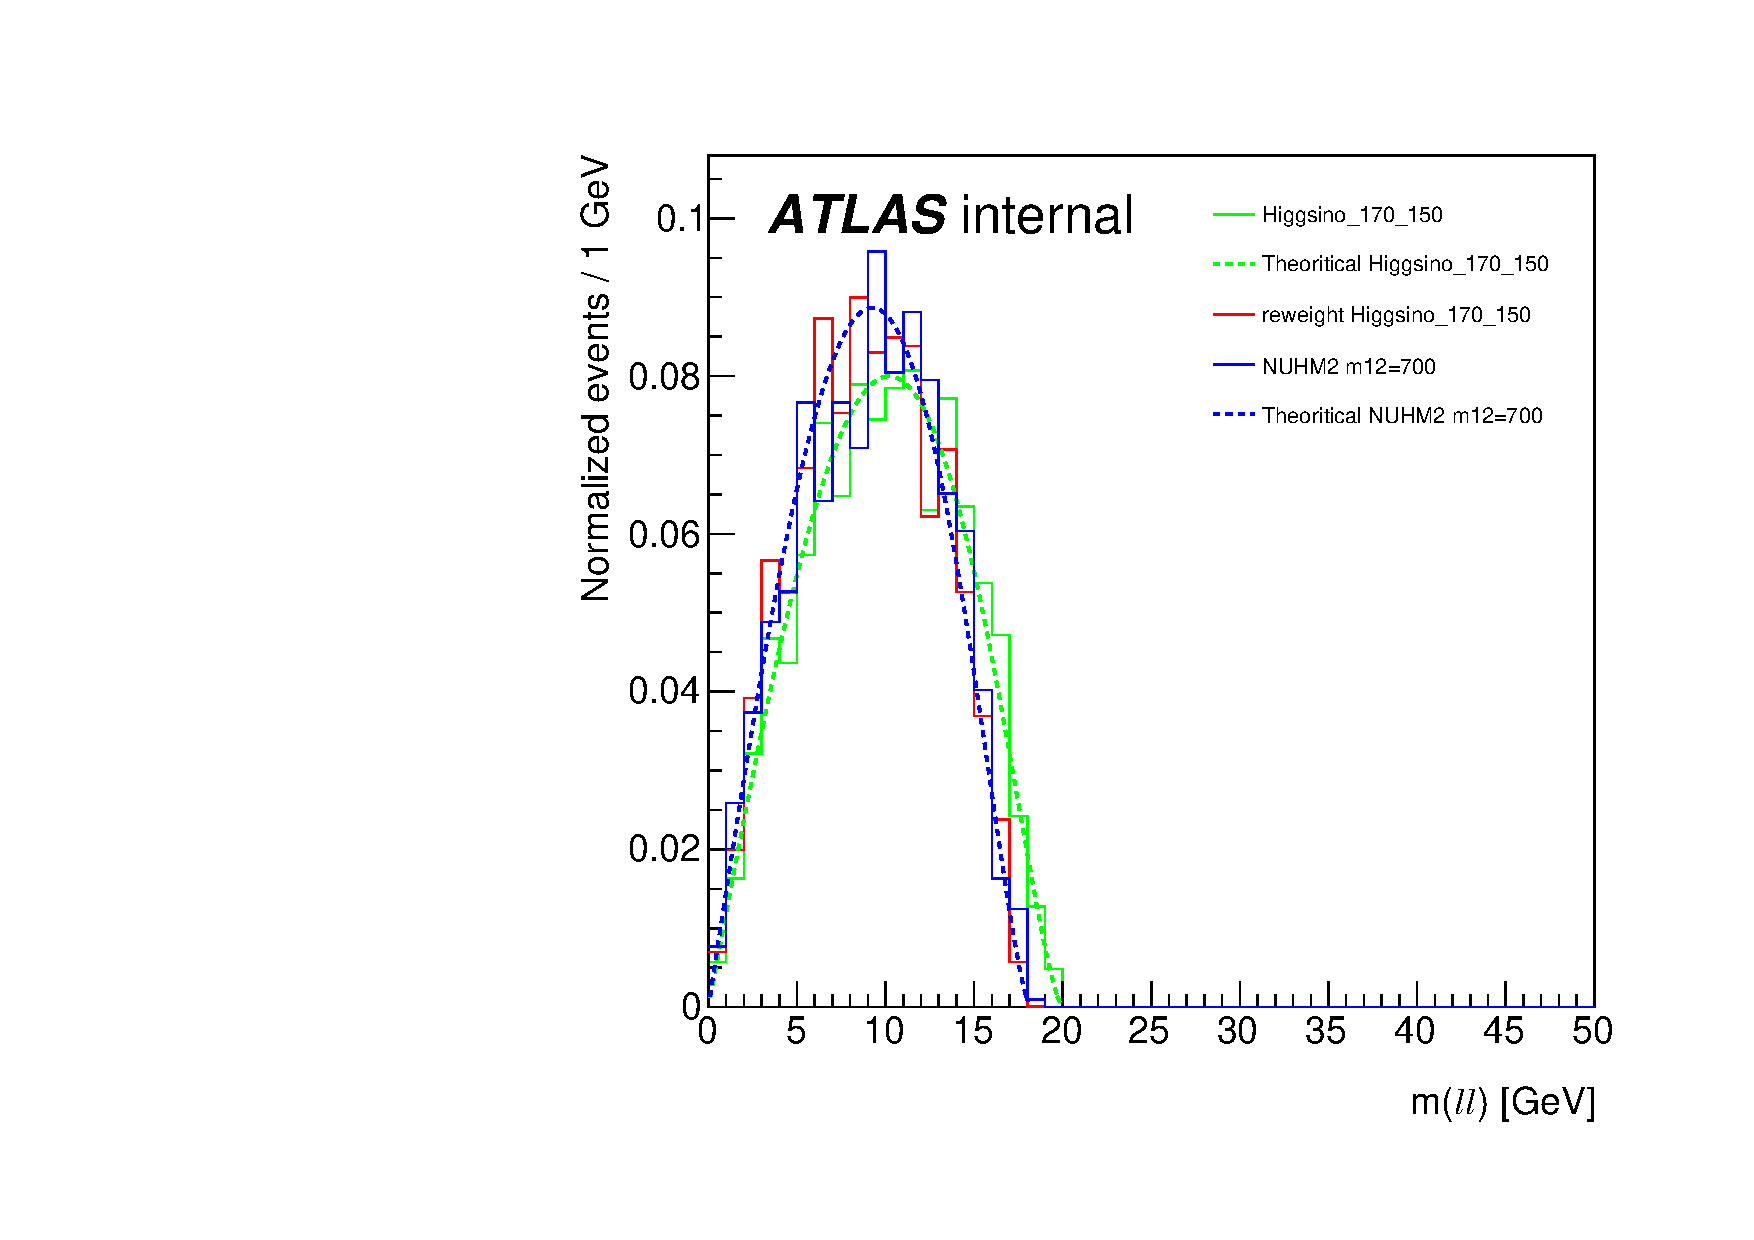
\includegraphics[scale=0.25]{reweight_Lorenzo_Higgsino_170_150_m12_700.pdf}
            \caption{NUHM2 $m_{1/2}=800$~{\GeV}}
        \end{subfigure}
    \end{center}
    \caption{The $m_{\ell \ell}$ distributions before and after reweighting for NUHM2 and the simplified Higgsino model.
    The blue and green solid lines are the TRUTH $m_{\ell \ell}$ distributions and the dashed lines are the distributions obtained from the Eq.~\ref{eq:results_mll_formula}.
    The good agreement between solid and dashed lines indicate the robustness of the formula.
    The red line is the event-by-event reweighting of the simplified Higgsino to the NUHM2 $m_{\ell \ell}$ which agrees with the prediction (blue dashed line).}
    \label{fig:results_nuhm2_reweighting}
\end{figure}

%%%
%%%
%%%

\subsection{The validation of $m_{\ell \ell}$ reweighting method}
\label{subsec:results_reweighted_validations}
The $m_{\ell \ell}$ reweighting method is validated by examining all kinematic variable distributions of NUHM2, simplified Higgsino, and reweighted Higgsino samples in truth level for all NUHM2 mass points.
Figures~\ref{fig:results_nuhm2_reweighting_validation_1} to \ref{fig:results_nuhm2_reweighting_validation_5} show the kinematic variable distributions for NUHM2 with $m_{1/2} = 700$~{\GeV}, simplified Higgsino with $m_{\widetilde{\chi}^{0}_{2}} = 170$ and $m_{\widetilde{\chi}^{0}_{1}} = 150$~{\GeV}, and reweighted Higgsino samples.
The distributions for the other $m_{1/2}$ mass points can be found in the App.~\ref{app:distributions}.
Good agreement between the NUHM2 and reweighted Higgsino samples can be found for all NUHM2 mass points.
The agreement is better if the $\delta = \Delta m_{Higgsino} - \Delta m_{NUHM2}$ is smaller.
Therefore, the reweighted Higgsino samples are used for the NUHM2 interpretation.

\begin{figure}[htbp]
    \begin{center}
        \begin{subfigure}[b]{0.48\textwidth}
            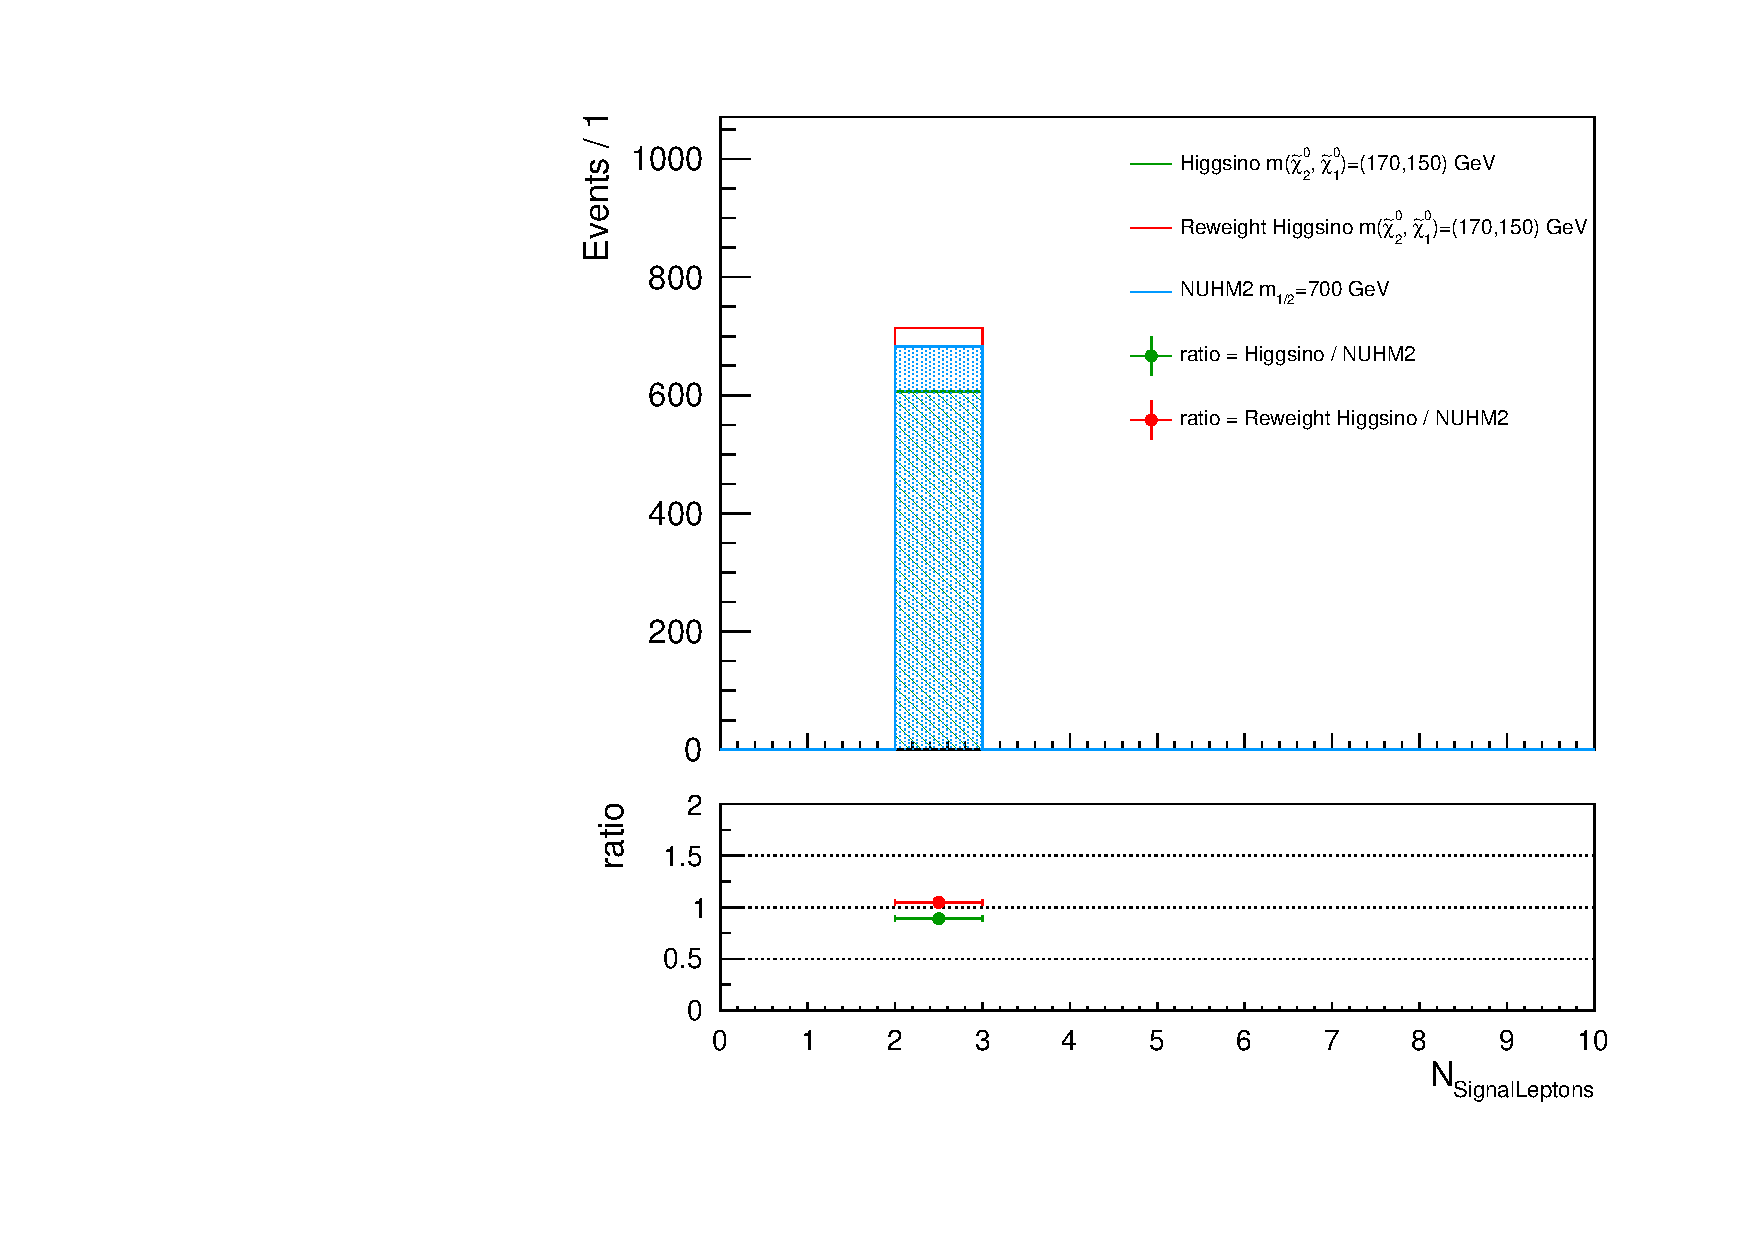
\includegraphics[scale=0.35]{reweight_Higgsino_170_150_m12_700_nSignalLeptons.pdf}
            \caption{Signal lepton multiplicity}
        \end{subfigure}
        \begin{subfigure}[b]{0.48\textwidth}
            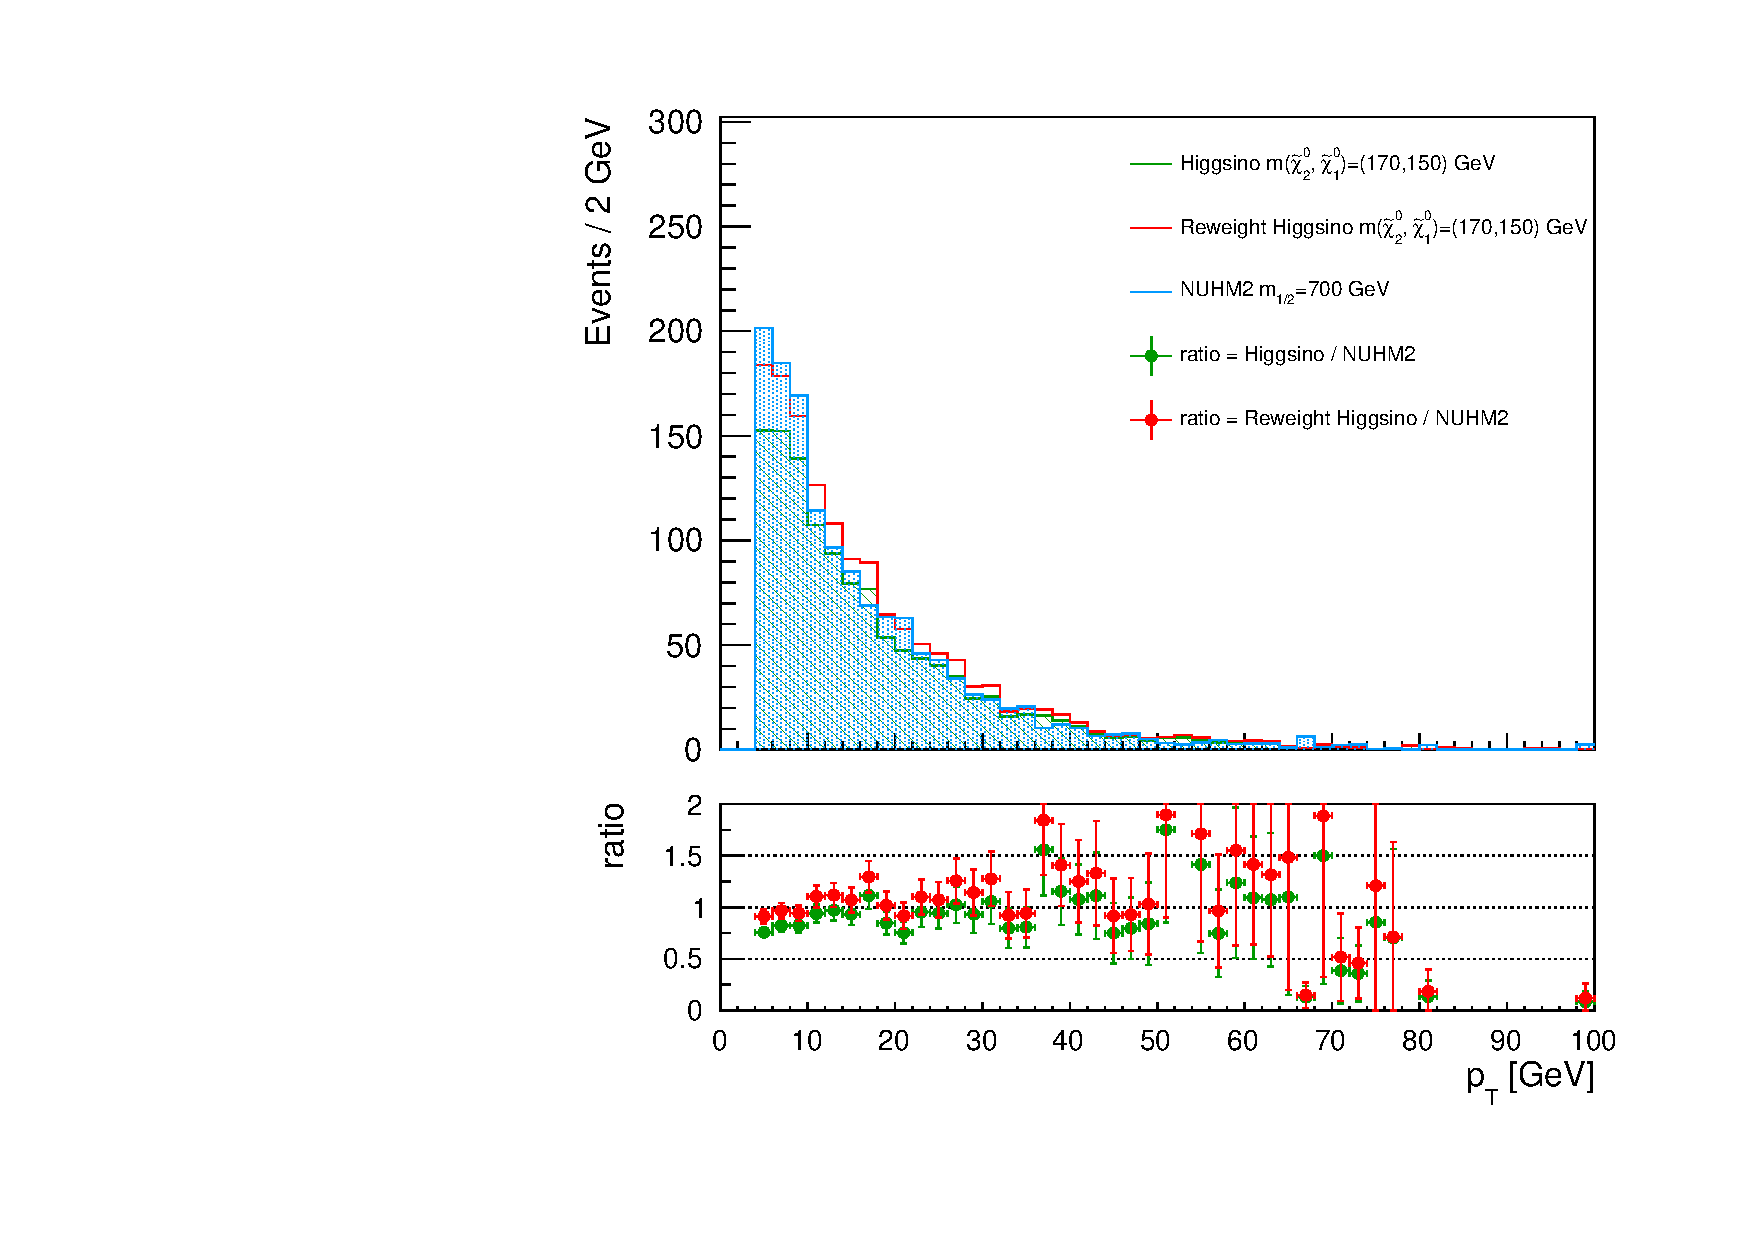
\includegraphics[scale=0.35]{reweight_Higgsino_170_150_m12_700_signalLeptons_pt.pdf}
            \caption{Signal lepton \pt}
        \end{subfigure}
        \begin{subfigure}[b]{0.48\textwidth}
            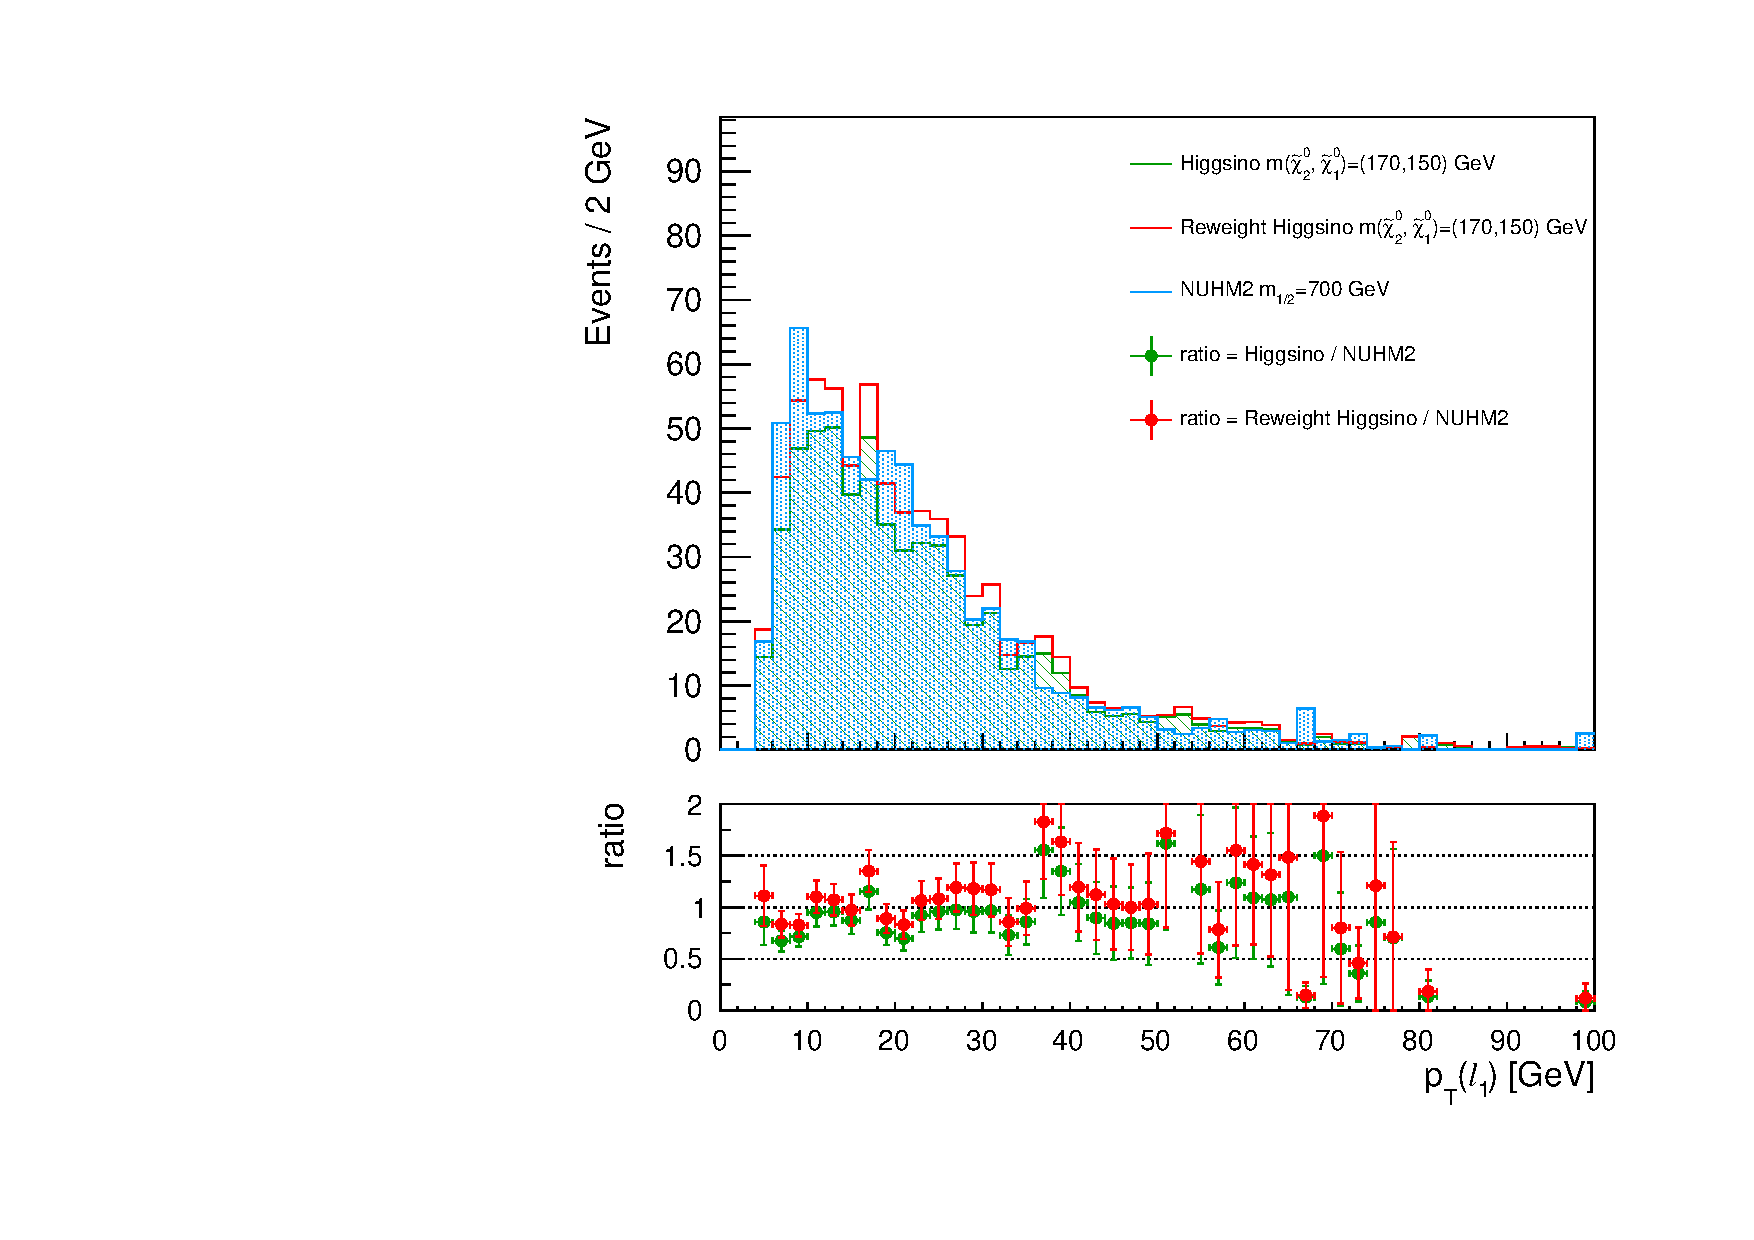
\includegraphics[scale=0.35]{reweight_Higgsino_170_150_m12_700_pTLep1.pdf}
            \caption{Leading lepton \pt}
        \end{subfigure}
        \begin{subfigure}[b]{0.48\textwidth}
            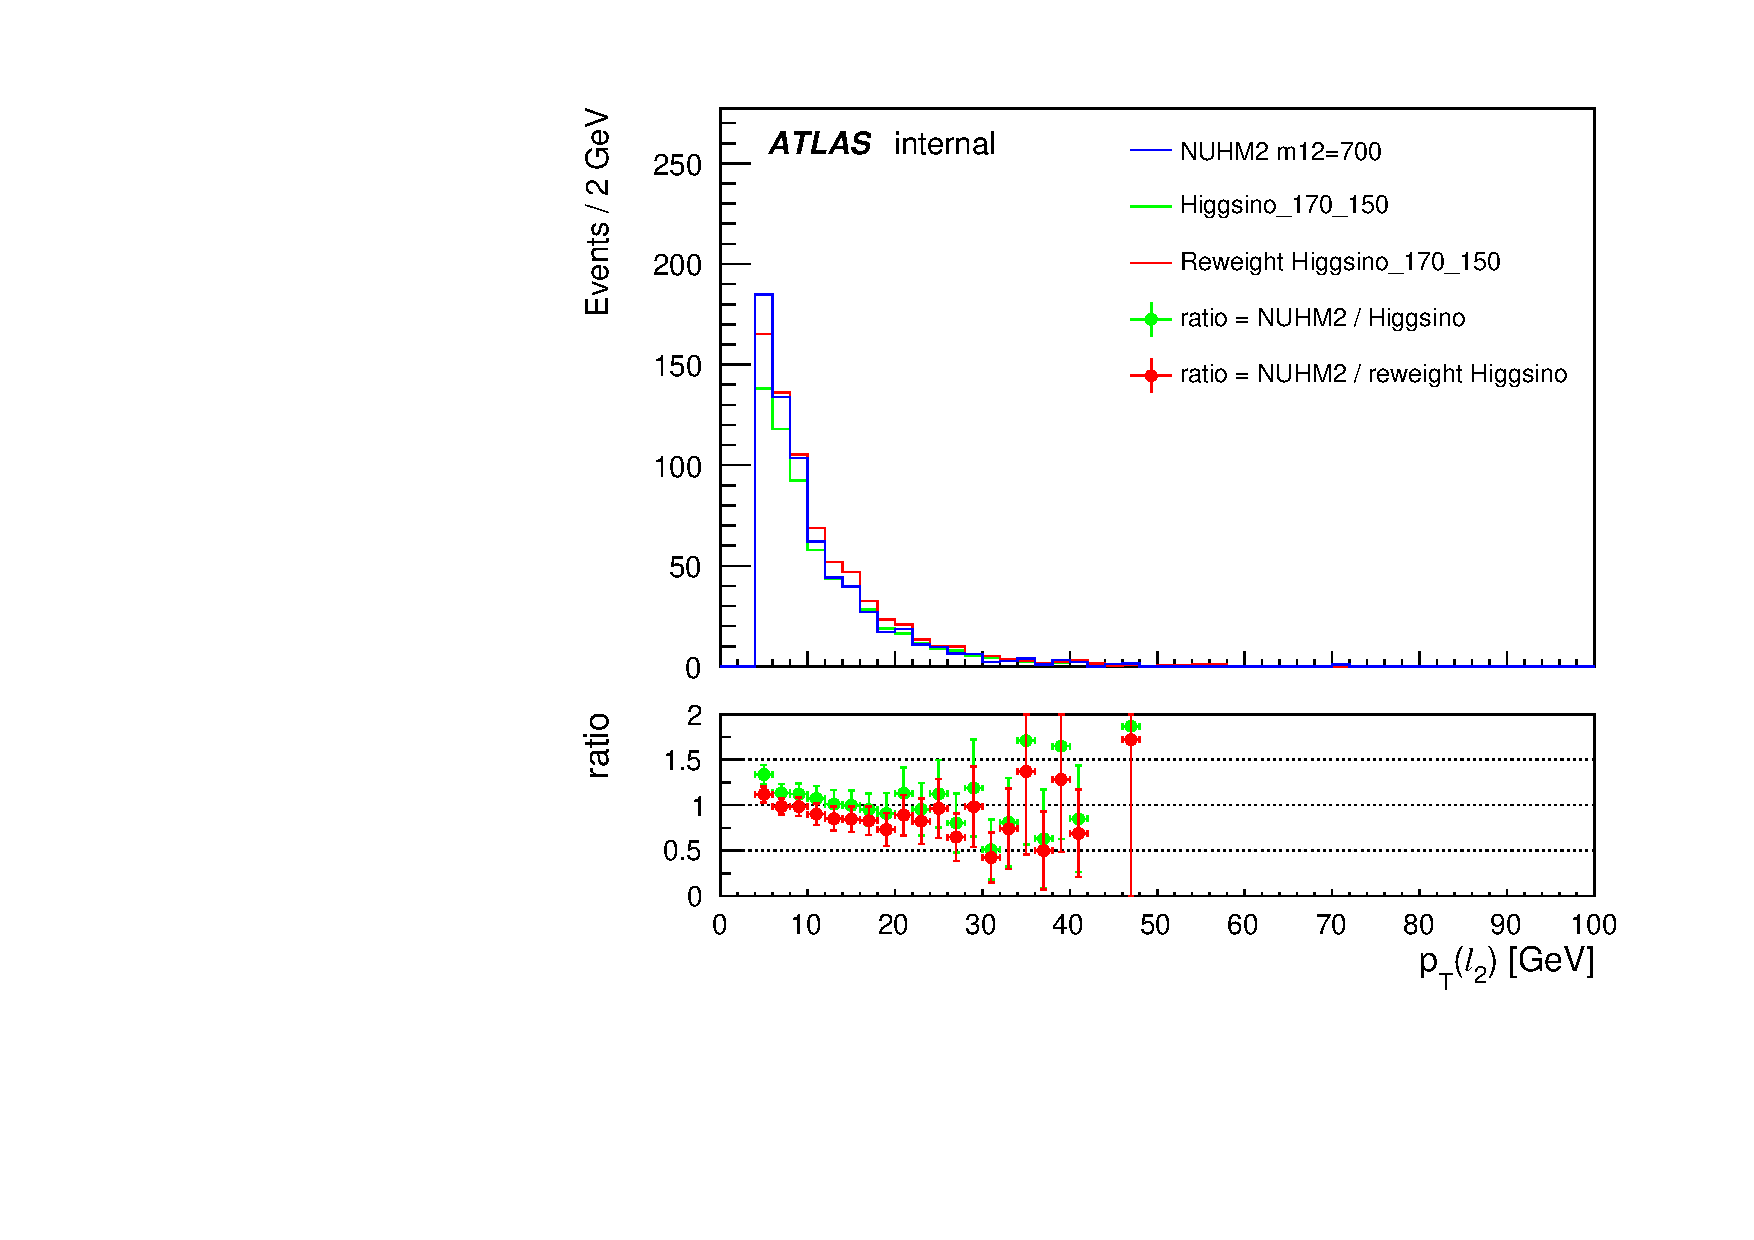
\includegraphics[scale=0.35]{reweight_Higgsino_170_150_m12_700_pTLep2.pdf}
            \caption{Subleading lepton \pt}
        \end{subfigure}
    \end{center}
    \caption{The distributions for signal lepton multiplicity, all signal leptons \pt, the leading lepton \pt, and the subleading lepton \pt.
    The NUHM2 signal sample uses  $m_{1/2} = 700$~{\GeV} and the Higgsino signal sample uses $m_{\widetilde{\chi}^{0}_{2}} = 170$ and $m_{\widetilde{\chi}^{0}_{1}} = 150$~{\GeV}.
    The reweighted Higgsino sample is shown in red line.
    The lower pad shows the ratio between NUHM2 and Higgsino (or reweighted Higgsino) distributions.}
    \label{fig:results_nuhm2_reweighting_validation_1}
\end{figure}

\begin{figure}[htbp]
    \begin{center}
        \begin{subfigure}[b]{0.48\textwidth}
            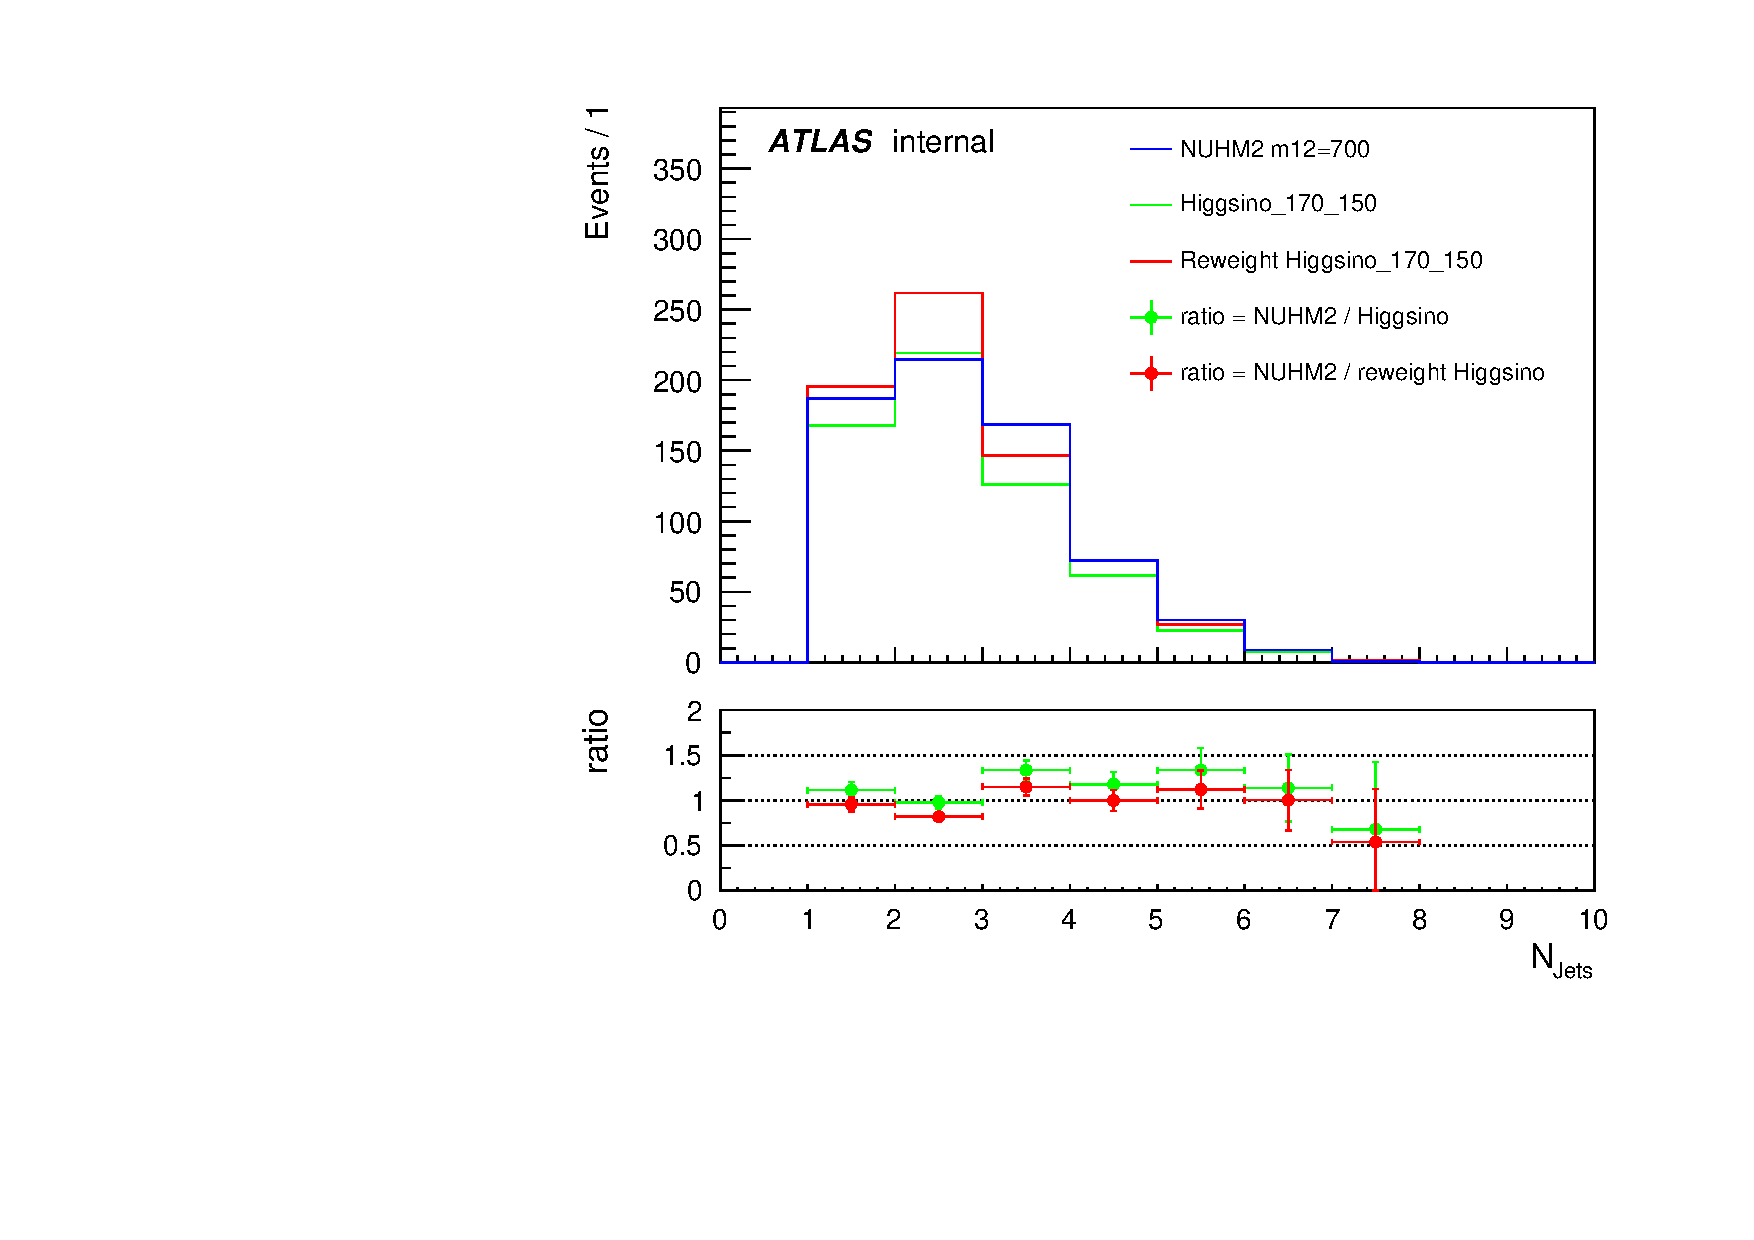
\includegraphics[scale=0.35]{reweight_Higgsino_170_150_m12_700_nJets.pdf}
            \caption{Jet multiplicity}
        \end{subfigure}
        \begin{subfigure}[b]{0.48\textwidth}
            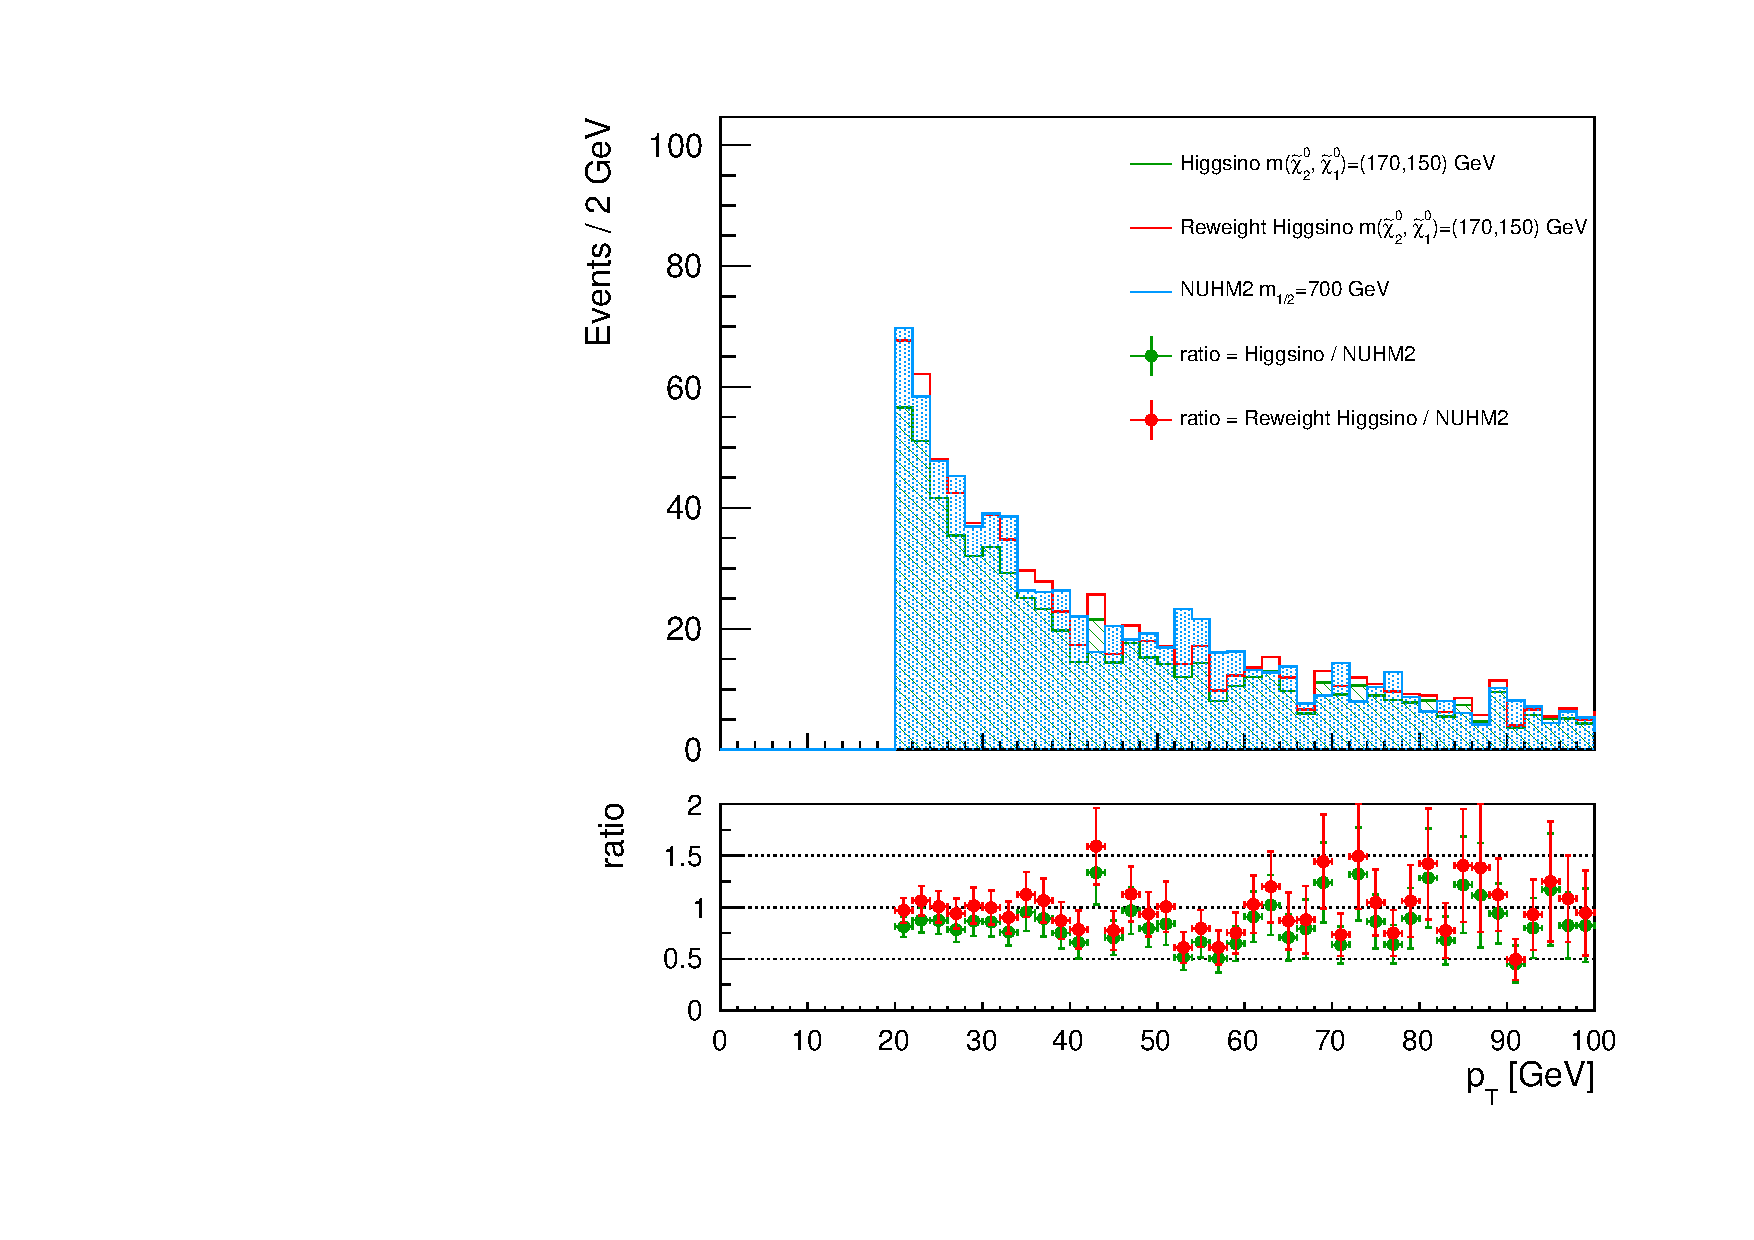
\includegraphics[scale=0.35]{reweight_Higgsino_170_150_m12_700_signalJets_pt.pdf}
            \caption{Jet \pt}
        \end{subfigure}
        \begin{subfigure}[b]{0.48\textwidth}
            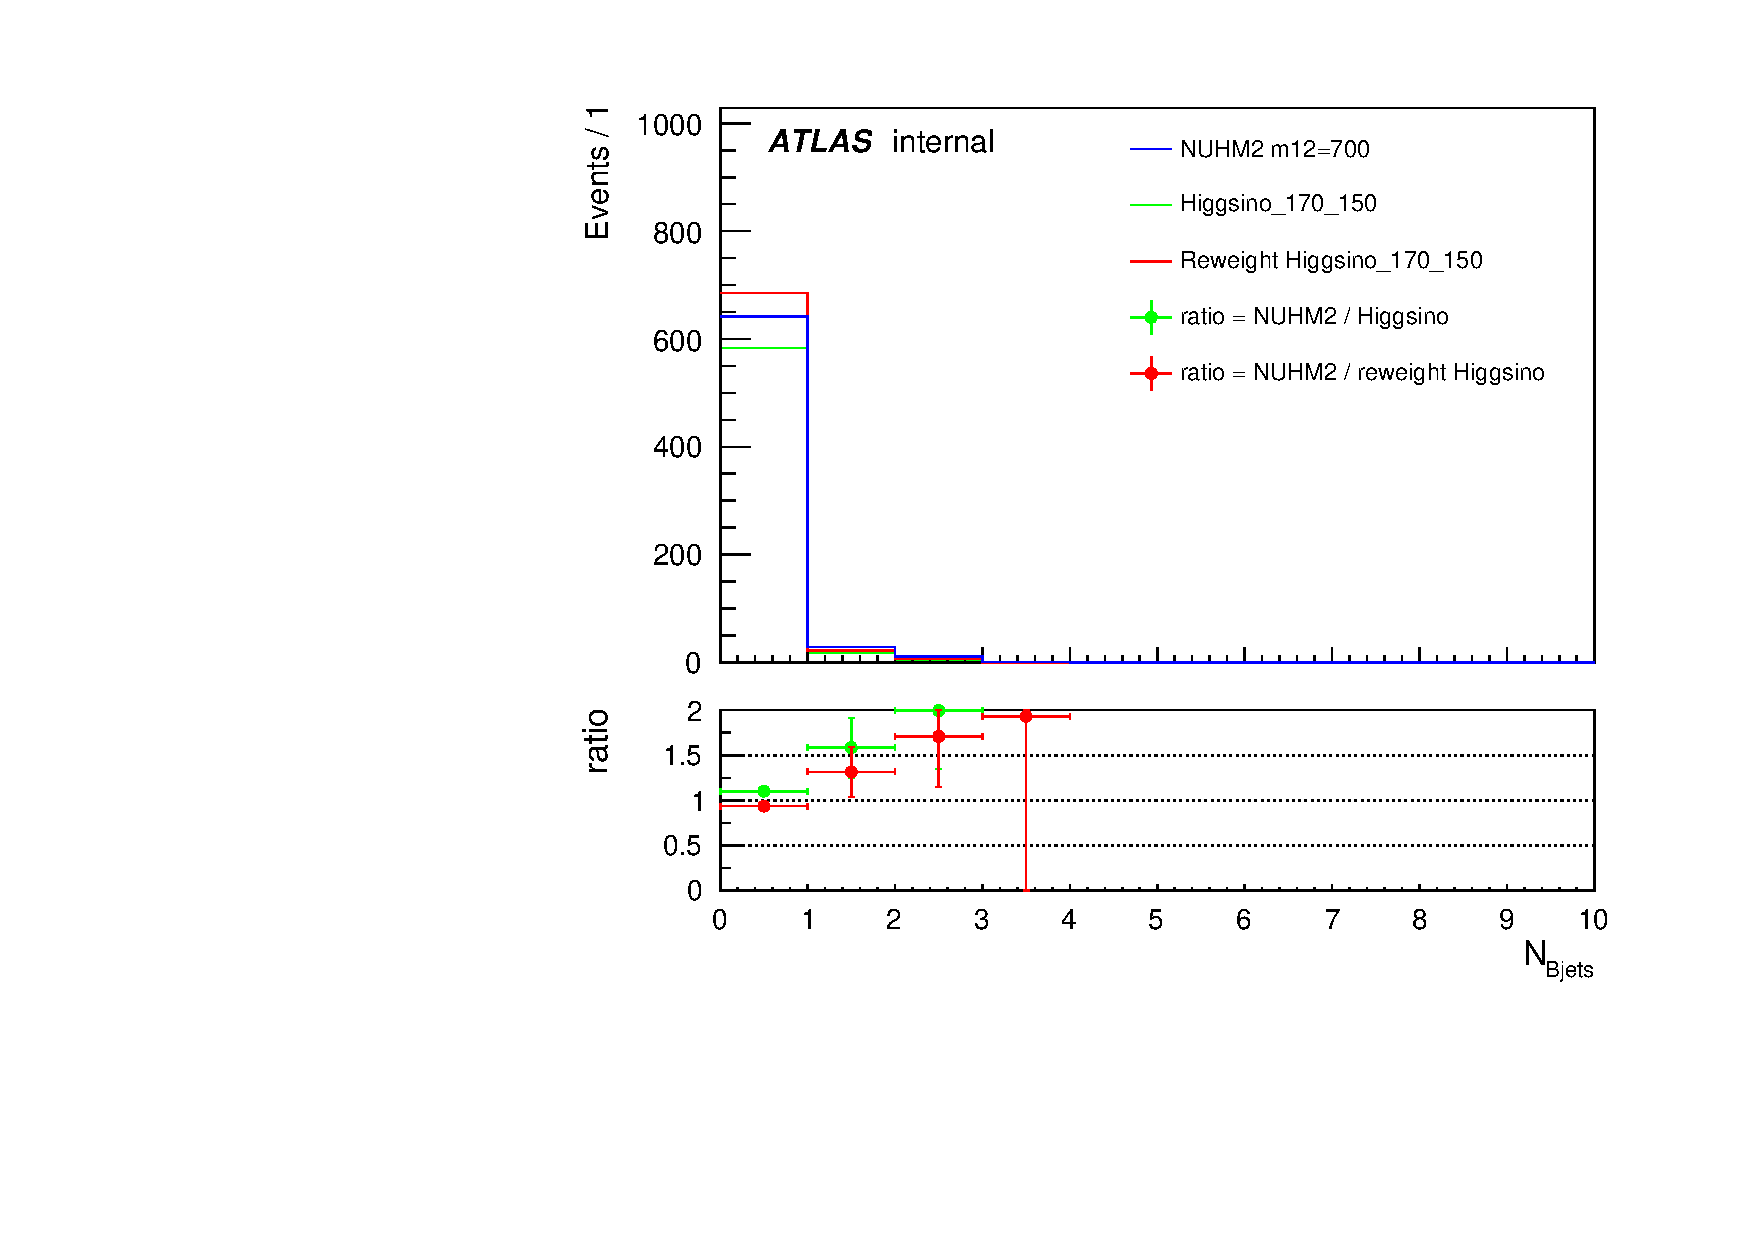
\includegraphics[scale=0.35]{reweight_Higgsino_170_150_m12_700_nBjets.pdf}
            \caption{$b$-jets multiplicity}
        \end{subfigure}
        \begin{subfigure}[b]{0.48\textwidth}
            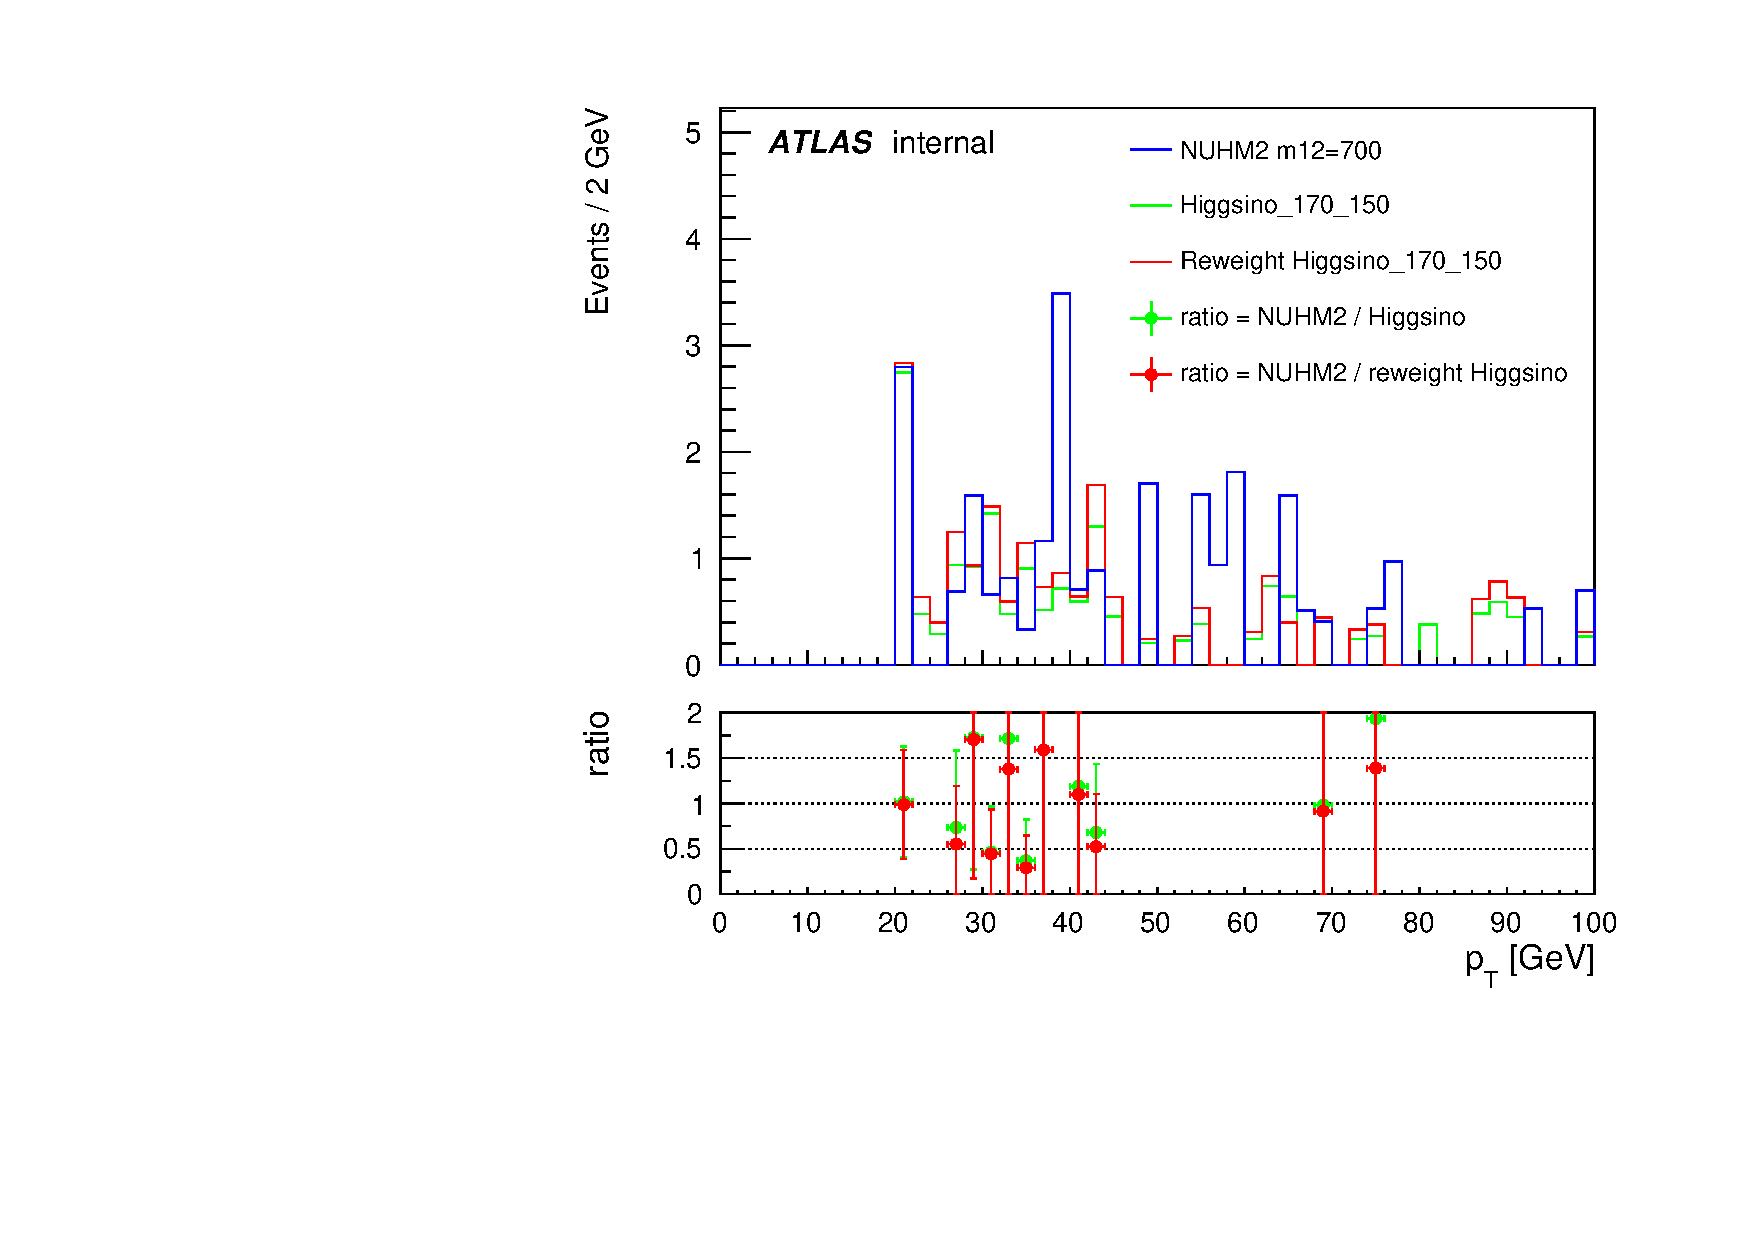
\includegraphics[scale=0.35]{reweight_Higgsino_170_150_m12_700_signalBjets_pt.pdf}
            \caption{$b$-jets \pt}
        \end{subfigure}
    \end{center}
    \caption{The distributions for jet multiplicity, jet \pt, $b$-jets multiplicity, and $b$-jet \pt.
    The NUHM2 signal sample uses  $m_{1/2} = 700$~{\GeV} and the Higgsino signal sample uses $m_{\widetilde{\chi}^{0}_{2}} = 170$ and $m_{\widetilde{\chi}^{0}_{1}} = 150$~{\GeV}.
    The reweighted Higgsino sample is shown in red line.
    The lower pad shows the ratio between NUHM2 and Higgsino (or reweighted Higgsino) distributions.}
    \label{fig:results_nuhm2_reweighting_validation_2}
\end{figure}

\begin{figure}[htbp]
    \begin{center}
        \begin{subfigure}[b]{0.48\textwidth}
            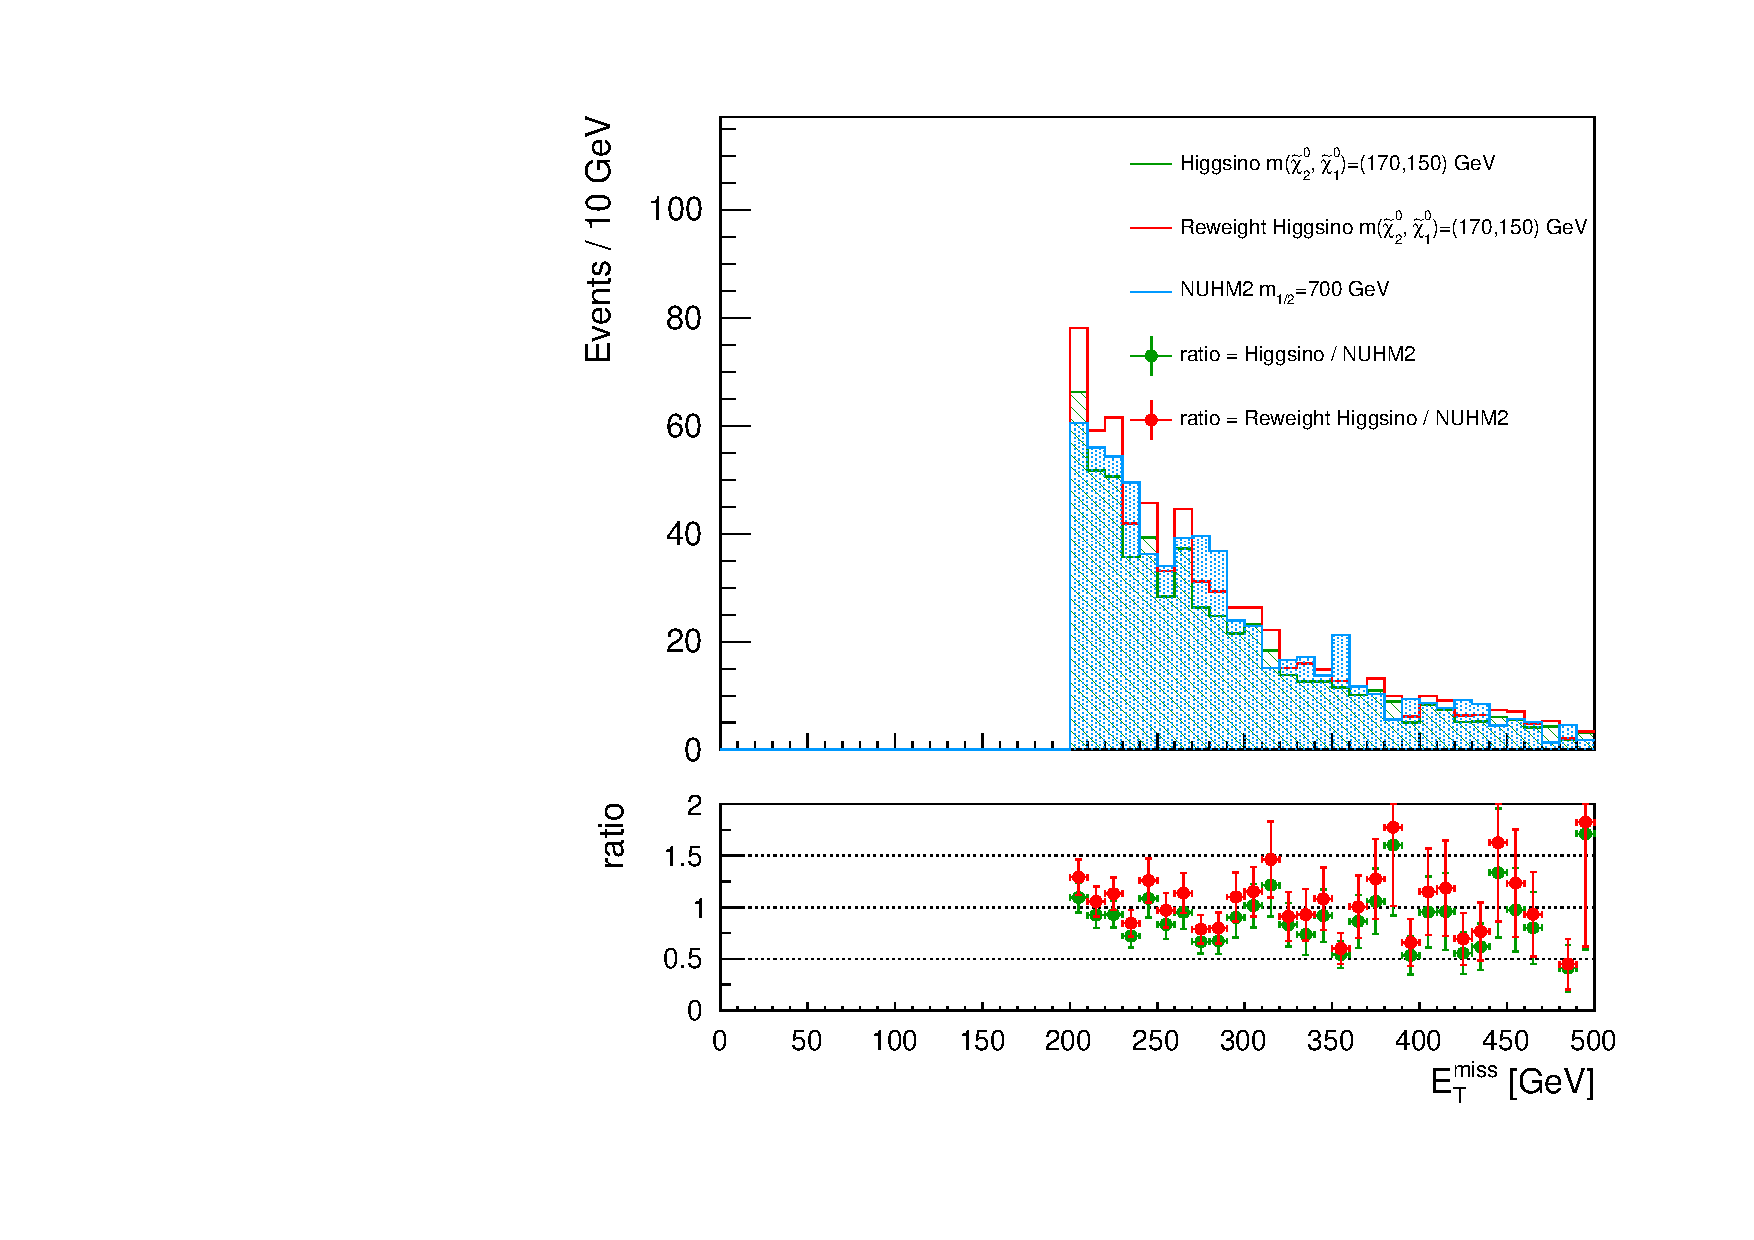
\includegraphics[scale=0.35]{reweight_Higgsino_170_150_m12_700_met.pdf}
            \caption{\met}
        \end{subfigure}
        \begin{subfigure}[b]{0.48\textwidth}
            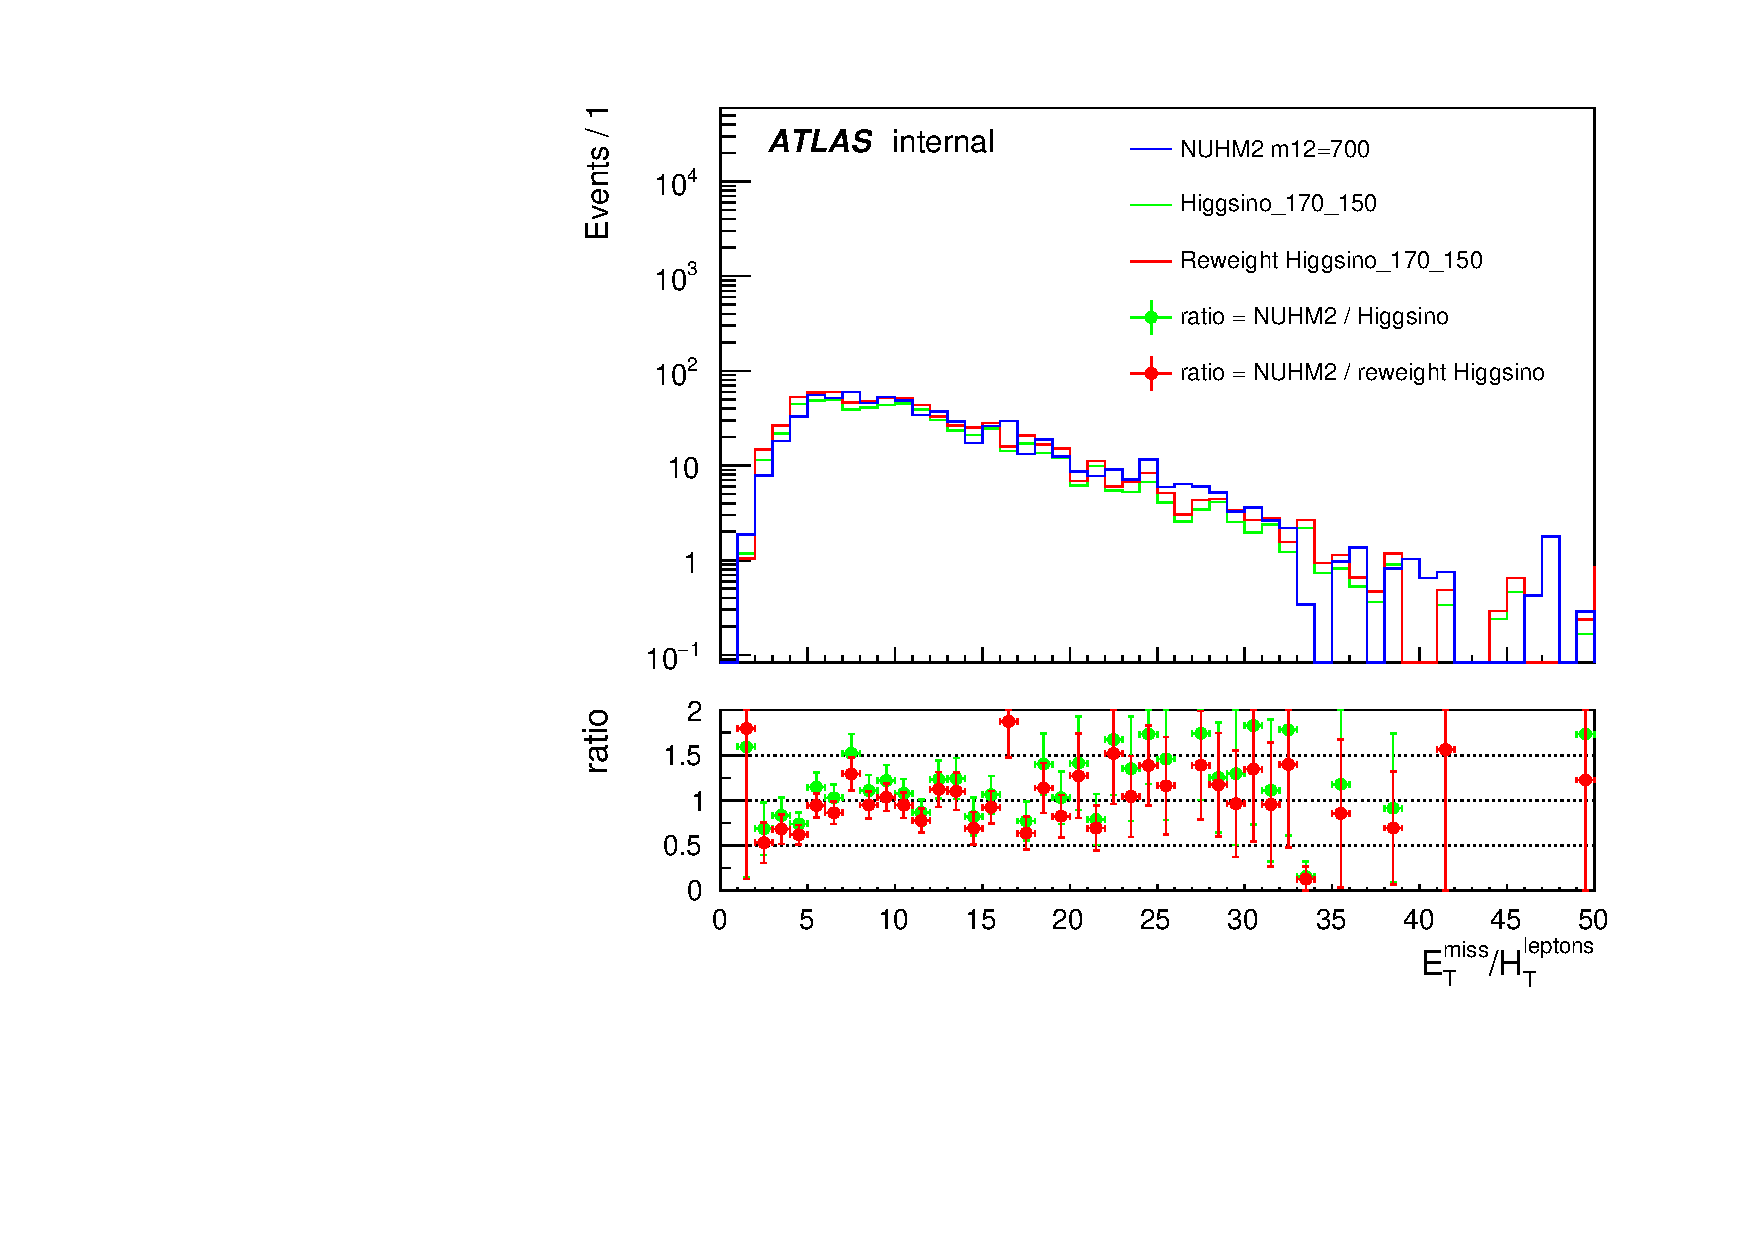
\includegraphics[scale=0.35]{reweight_Higgsino_170_150_m12_700_METOverHTLep12.pdf}
            \caption{$\met/H^\mathrm{leptons}_\mathrm{T}$}
        \end{subfigure}
        \begin{subfigure}[b]{0.48\textwidth}
            \includegraphics[scale=0.35]{reweight_Higgsino_170_150_m12_700_mll.pdf}
            \caption{$m_{\ell \ell}$}
        \end{subfigure}
        \begin{subfigure}[b]{0.48\textwidth}
            \includegraphics[scale=0.35]{reweight_Higgsino_170_150_m12_700_MTauTau.pdf}
            \caption{$m_{\tau \tau}$}
        \end{subfigure}
    \end{center}
    \caption{The distributions for \met, $\met/H^\mathrm{leptons}_\mathrm{T}$, $m_{\ell \ell}$, and $m_{\tau \tau}$.
    The NUHM2 signal sample uses  $m_{1/2} = 700$~{\GeV} and the Higgsino signal sample uses $m_{\widetilde{\chi}^{0}_{2}} = 170$ and $m_{\widetilde{\chi}^{0}_{1}} = 150$~{\GeV}.
    The reweighted Higgsino sample is shown in red line.
    The lower pad shows the ratio between NUHM2 and Higgsino (or reweighted Higgsino) distributions.}
    \label{fig:results_nuhm2_reweighting_validation_3}
\end{figure}

\begin{figure}[htbp]
    \begin{center}
        \begin{subfigure}[b]{0.48\textwidth}
            \includegraphics[scale=0.35]{reweight_Higgsino_170_150_m12_700_mT.pdf}
            \caption{$m_\mathrm{T}$}
        \end{subfigure}
        \begin{subfigure}[b]{0.48\textwidth}
            \includegraphics[scale=0.35]{reweight_Higgsino_170_150_m12_700_mT2.pdf}
            \caption{$m_\mathrm{T2}$}
        \end{subfigure}
        \begin{subfigure}[b]{0.48\textwidth}
            \includegraphics[scale=0.35]{reweight_Higgsino_170_150_m12_700_meffIncl.pdf}
            \caption{$m^\mathrm{Incl}_\mathrm{eff}$}
        \end{subfigure}
        \begin{subfigure}[b]{0.48\textwidth}
            \includegraphics[scale=0.35]{reweight_Higgsino_170_150_m12_700_HTIncl.pdf}
            \caption{$H^\mathrm{Incl}_\mathrm{T}$}
        \end{subfigure}
    \end{center}
    \caption{The distributions for $m_\mathrm{T}$, $m_\mathrm{T2}$, $m^\mathrm{Incl}_\mathrm{eff}$, $H^\mathrm{Incl}_\mathrm{T}$.
    The NUHM2 signal sample uses  $m_{1/2} = 700$~{\GeV} and the Higgsino signal sample uses $m_{\widetilde{\chi}^{0}_{2}} = 170$ and $m_{\widetilde{\chi}^{0}_{1}} = 150$~{\GeV}.
    The reweighted Higgsino sample is shown in red line.
    The lower pad shows the ratio between NUHM2 and Higgsino (or reweighted Higgsino) distributions.}
    \label{fig:results_nuhm2_reweighting_validation_4}
\end{figure}

\begin{figure}[htbp]
    \begin{center}
        \begin{subfigure}[b]{0.48\textwidth}
            \includegraphics[scale=0.35]{reweight_Higgsino_170_150_m12_700_Rll.pdf}
            \caption{$\Delta R_{\ell \ell}$}
        \end{subfigure}
        \begin{subfigure}[b]{0.48\textwidth}
            \includegraphics[scale=0.35]{reweight_Higgsino_170_150_m12_700_dphiMin1.pdf}
            \caption{$\Delta \phi(\mathbf{p}^\mathrm{j1}_\mathrm{T}, \mathbf{p}^\mathrm{miss}_\mathrm{T})$}
        \end{subfigure}
    \end{center}
    \caption{The distributions for $\Delta R_{\ell \ell}$ and $\Delta \phi(\mathbf{p}^\mathrm{j1}_\mathrm{T}, \mathbf{p}^\mathrm{miss}_\mathrm{T})$.
    The NUHM2 signal sample uses  $m_{1/2} = 700$~{\GeV} and the Higgsino signal sample uses $m_{\widetilde{\chi}^{0}_{2}} = 170$ and $m_{\widetilde{\chi}^{0}_{1}} = 150$~{\GeV}.
    The reweighted Higgsino sample is shown in red line.
    The lower pad shows the ratio between NUHM2 and Higgsino (or reweighted Higgsino) distributions.}
    \label{fig:results_nuhm2_reweighting_validation_5}
\end{figure}

%%%
%%%
%%%

\subsection{NUHM2 interpretation using the $m_{\ell \ell}$ reweighting}
\label{subsec:results_mll_reweighting_interpretation}
The NUHM2 interpretation is performed using the reweighted Higgsino samples to obtain the NUHM2 distributions at the reconstruction level.
All systematic uncertainties are considered in the calculation.
The upper limits of the cross-section combining $\widetilde{\chi}^{0}_{2} \widetilde{\chi}^{0}_{1}$, $\widetilde{\chi}^{0}_{2} \widetilde{\chi}^{\pm}_{1}$, and $\widetilde{\chi}^{\pm}_{1} \widetilde{\chi}^{\mp}_{1}$ productions are shown in Fig.~\ref{fig:results_nuhm2_interpretation_reweighting}.
The upper limits of cross-section are labeled by the gray number on each $m_{1/2}$ and the lower axis shows the $\Delta m = m_{\widetilde{\chi}^{0}_{2}} - m_{\widetilde{\chi}^{0}_{1}}$.
None of the NUHM2 $m_{1/2}$ points are excluded at the 95\% CL.

\begin{figure}[htb]
    \begin{center}
        \includegraphics[scale=0.4]{nuhm2_UL_rew.pdf}
        \caption{The upper limits of the cross-section for NUHM2 using the $m_{\ell \ell}$ reweighting method.}
        \label{fig:results_nuhm2_interpretation_reweighting}
    \end{center}
\end{figure}

%%%
%%%
%%%

\section{NUHM2 interpretation using the MC production}
\label{sec:results_mc_production_interpretation}
Although the NUHM2 interpretation using the $m_{\ell \ell}$ reweighting Higgsino samples is shown in Sect.~\ref{subsec:results_mll_reweighting_interpretation}, the final results must be determined using the MC production samples.
The NUHM2 signal MC production has been mentioned in Sect.~\ref{subsubsec:data_NUHM2_generation} and the signal region selection is described in Sect.~\ref{subsec:event_signal_region}.
The kinematic distributions in the SR$\ell \ell$-$m_{\ell \ell}$ are shown in Figs.~\ref{fig:event_nuhm2_kinematic_in_SR_SFOS_1}, \ref{fig:event_nuhm2_kinematic_in_SR_SFOS_2}, and \ref{fig:event_nuhm2_kinematic_in_SR_SFOS_3} and the yields are provided in Tables~\ref{tab:event_cutflow_NUHM2_1} and \ref{tab:event_cutflow_NUHM2_2}.
The statistical interpretation is performed using the HiggsinoFitter which wraps the HistFitter~\cite{Baak:2014wma}.
Table~\ref{tab:results_nuhm2_cls} shows the calculated CLs values for NUHM2 with and without systematic uncertainties.

\begin{table}[htp]
    \begin{center}
        {\footnotesize
            \begin{tabular}{cllll}
                \hline
                \hline
                \multirow{2}{*}{$m_{1/2}$~[{\GeV}]} & \multicolumn{2}{c}{No systematics} & \multicolumn{2}{c}{All systematics}\\
                & $CLs_{obs}$ & $CLs_{exp}$ & $CLs_{obs}$ & $CLs_{exp}$\\
                \hline
                350 & 0.6199 & 0.5434 & 0.6458 & 0.6007\\
                400 & 0.5549 & 0.5233 & 0.5567 & 0.5844\\
                500 & 0.3811 & 0.3556 & 0.4021 & 0.4494\\
                600 & 0.3417 & 0.2305 & 0.3808 & 0.3133\\
                700 & 0.2457 & 0.0879 & 0.2929 & 0.1362\\
                800 & 0.2037 & 0.0916 & 0.2265 & 0.1307\\
                \hline
                \hline
            \end{tabular}
        }
    \end{center}
    \caption{The calculated CLs values for NUHM2 with and without systematic uncertainties in the statistical interpretation.}
    \label{tab:results_nuhm2_cls}
\end{table}%
% \begin{table}[htp]
%     \begin{center}
%         {\footnotesize
%             \begin{tabular}{cllll}
%                 \hline
%                 \hline
%                 \multirow{2}{*}{$m_{1/2}$~[{\GeV}]} & \multicolumn{2}{c}{No systematics} & \multicolumn{2}{c}{All systematics}\\
%                 & $CLs_{obs}$ & $CLs_{exp}$ & $CLs_{obs}$ & $CLs_{exp}$\\
%                 \hline
%                 350 & 0.6198885 & 0.5434401 & 0.6458337 & 0.600724\\
%                 400 & 0.5549458 & 0.5232649 & 0.5566812 & 0.584395\\
%                 500 & 0.3811002 & 0.3555793 & 0.4021327 & 0.449390\\
%                 600 & 0.3417218 & 0.2305462 & 0.3808340 & 0.313335\\
%                 700 & 0.2457024 & 0.0879370 & 0.2929172 & 0.136177\\
%                 800 & 0.2036754 & 0.0915838 & 0.2265301 & 0.130744\\
%                 \hline
%                 \hline
%             \end{tabular}
%         }
%     \end{center}
%     \caption{The calculated CLs values for NUHM2 with and without systematic uncertainties in the statistical interpretation.}
%     \label{tab:results_nuhm2_cls}
% \end{table}%

In both cases with and without systematics, the $CLs_{obs}$ should be worse (higher) than the $CLs_{exp}$ due to a small excess observed in some $m_{\ell \ell}$ bins.
Two exceptions in NUHM2 $m_{1/2} = 400$ and 500~{\GeV} with all systematics are observed.
The $CLs_{exp}$ are slightly higher than $CLs_{obs}$ for these two mass points.
Since this situation is not seen in the without systematics case, this situation happens when there are increasing systematic uncertainties for these two $m_{1/2}$.
Although the exceptions exist, the $CLs_{obs}$ and $CLs_{exp}$ with and without systematics have good agreement.
Figure~\ref{fig:results_nuhm2_signal_strength} shows the signal strength $\mu_\mathrm{sig}$ for all NUHM2 points, all plots are consistent.

\begin{figure}[htbp]
    \begin{center}
        \begin{subfigure}[b]{0.48\textwidth}
            \includegraphics[scale=0.35]{upperlimit_cls_poi_MGPy8EG_A14N23LO_NUHM2_m12_350_weak_2LMET50_MadSpin_Asym_CLs_grid_ts3.pdf}
            \caption{NUHM2 $m_{1/2} = 350$~{\GeV}}
        \end{subfigure}
        \begin{subfigure}[b]{0.48\textwidth}
            \includegraphics[scale=0.35]{upperlimit_cls_poi_MGPy8EG_A14N23LO_NUHM2_m12_400_weak_2LMET50_MadSpin_Asym_CLs_grid_ts3.pdf}
            \caption{NUHM2 $m_{1/2} = 400$~{\GeV}}
        \end{subfigure}
        \begin{subfigure}[b]{0.48\textwidth}
            \includegraphics[scale=0.35]{upperlimit_cls_poi_MGPy8EG_A14N23LO_NUHM2_m12_500_weak_2LMET50_MadSpin_Asym_CLs_grid_ts3.pdf}
            \caption{NUHM2 $m_{1/2} = 500$~{\GeV}}
        \end{subfigure}
        \begin{subfigure}[b]{0.48\textwidth}
            \includegraphics[scale=0.35]{upperlimit_cls_poi_MGPy8EG_A14N23LO_NUHM2_m12_600_weak_2LMET50_MadSpin_Asym_CLs_grid_ts3.pdf}
            \caption{NUHM2 $m_{1/2} = 600$~{\GeV}}
        \end{subfigure}
        \begin{subfigure}[b]{0.48\textwidth}
            \includegraphics[scale=0.35]{upperlimit_cls_poi_MGPy8EG_A14N23LO_NUHM2_m12_700_weak_2LMET50_MadSpin_Asym_CLs_grid_ts3.pdf}
            \caption{NUHM2 $m_{1/2} = 700$~{\GeV}}
        \end{subfigure}
        \begin{subfigure}[b]{0.48\textwidth}
            \includegraphics[scale=0.35]{upperlimit_cls_poi_MGPy8EG_A14N23LO_NUHM2_m12_800_weak_2LMET50_MadSpin_Asym_CLs_grid_ts3.pdf}
            \caption{NUHM2 $m_{1/2} = 800$~{\GeV}}
        \end{subfigure}
    \end{center}
    \caption{The signal strength $\mu_\mathrm{sig}$ for the NUHM2 mass points.}
    \label{fig:results_nuhm2_signal_strength}
\end{figure}

The upper limit of the cross-section is calculated by
%
\begin{equation}
	\sigma_{UL} = \mu_\mathrm{sig} \times \big[ \sigma_{prod}(\widetilde{\chi}^{0}_{2} \widetilde{\chi}^{0}_{1}) + \sigma_{prod}(\widetilde{\chi}^{0}_{2} \widetilde{\chi}^{+}_{1}) + \sigma_{prod}(\widetilde{\chi}^{0}_{2} \widetilde{\chi}^{-}_{1}) + \sigma_{prod}(\widetilde{\chi}^{\pm}_{1} \widetilde{\chi}^{\mp}_{1}) \big] \quad ,
\end{equation}
%
where $\mu_\mathrm{sig}$ is the signal strength, and the four $\sigma_{prod}$ are the cross-sections for different productions at next-to-leading-logarithm (NLL) accuracy.
The upper limits of the cross-section with and without systematics are plotted in Fig.~\ref{fig:results_nuhm2_interpretation_mc_production}.
The gray numbers are the upper limits of the cross-section in pb.
The all systematics case has higher upper limits than the one without systematics as expected.
None of the NUHM2 $m_{1/2}$ points are excluded at the 95\% CL and the observed upper limits have higher then the theoretical prediction.

\begin{figure}[htbp]
    \begin{center}
        \begin{subfigure}[b]{0.48\textwidth}
            \includegraphics[scale=0.35]{nuhm2_UL_mcprod_NoSys.pdf}
            \caption{No systematics}
        \end{subfigure}
        \begin{subfigure}[b]{0.48\textwidth}
            \includegraphics[scale=0.35]{nuhm2_UL_mcprod_AllSys.pdf}
            \caption{All systematics}
        \end{subfigure}
    \end{center}
    \caption{The upper limit of the cross-section of NUHM2 for with and without systematics.
    The gray numbers are the upper limits in pb.}
    \label{fig:results_nuhm2_interpretation_mc_production}
\end{figure}
